%------------------------------------------------------------------------------
%
% Tec 教科書
%
%------------------------------------------------------------------------------
\documentclass[a4paper,twocolumn,twoside]{ltjsbook}   % lualatex の場合
%----------- 印刷版とPDF版の区別 ----------------------------------------------
\newif\ifPDF
%\PDFfalse    %印刷版の場合
\PDFtrue      %PDF版の場合
%------------------------------------------------------------------------------
\ifPDF
\newcommand{\pdf}{(PDF版)}
\else
\newcommand{\pdf}{}
\fi
%------------------------------------------------------------------------------
\usepackage{tec}
\newcommand{\edition}{第4版}
\newcommand{\ver}{Ver. 4.1.0}
%------------------------------------------------------------------------------
% はじまり
\begin{document}
%------------------------------------------------------------------------------
% カバー
\setcounter{page}{0}
\thispagestyle{empty}
\onecolumn
~
\vfill
\vfill
{\noindent
\fontsize{34pt}{50pt}\selectfont\textbf{TeC教科書}
}
\vfill
\vfill
\centerline{
  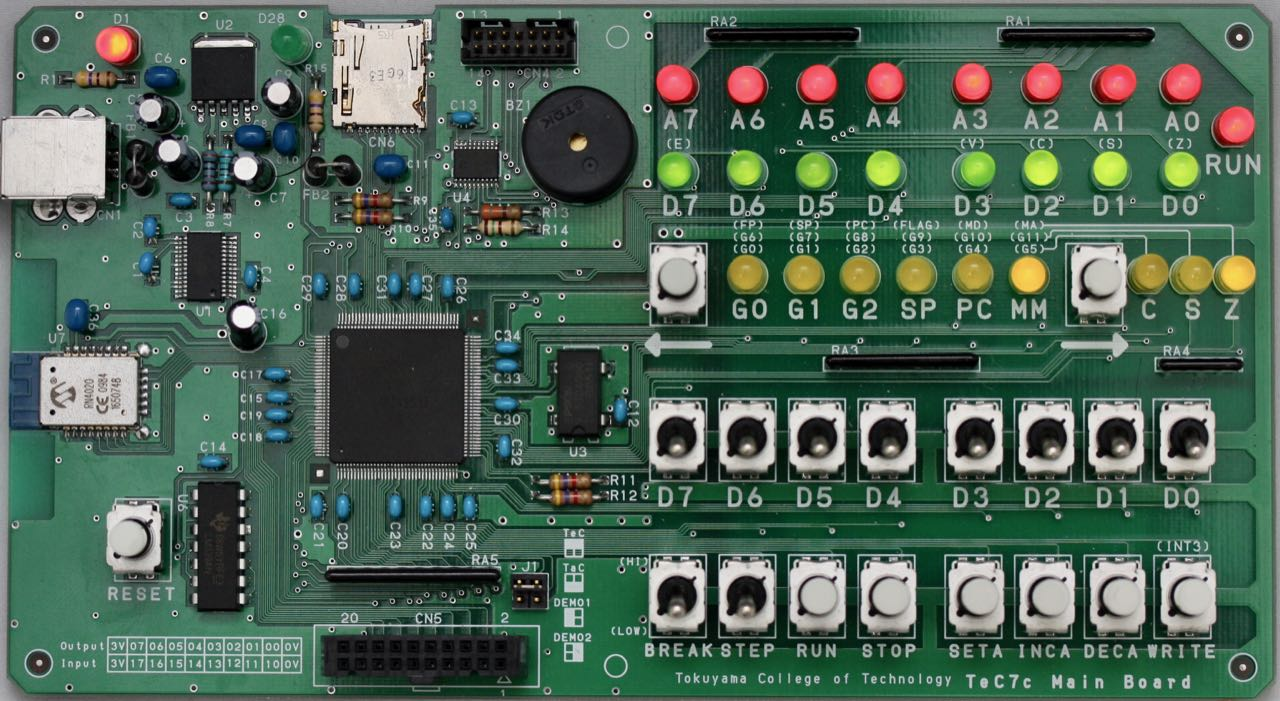
\includegraphics[scale=0.38]{Img/TeC7c.jpg}
}
\vfill
\vfill
\centerline{\Large 徳山工業高等専門学校 情報電子工学科}
%\centerline{\Large 重村研究室}
\centerline{\Large\ttfamily https://github.com/tctsigemura/TeC7}
\vfill

%------------------------------------------------------------------------------
\ifPDF
\newpage
\setcounter{page}{0}
\thispagestyle{empty}
\onecolumn
~
\fi

%------------------------------------------------------------------------------
% 表紙
\frontmatter
\title{TeC 教科書\\\ver}
\author{徳山工業高等専門学校\\情報電子工学科\\TeCプロジェクト\\
\url{https://github.com/tctsigemura/TeC7}}
\date{}
\maketitle

%------------------------------------------------------------------------------
% 著作権表示
\thispagestyle{empty}
\onecolumn
~
\vfill
\begin{flushleft}
Copyright \copyright ~~ 2017 - 2019 by \\
Dept. of Computer Science and Electronic Engineering, \\
Tokuyama College of Technology, JAPAN
\end{flushleft}
\vspace{0.4cm}
\begin{flushleft}
本書の一部は,JSPS 科研費 22500833 および 16K0099 の
助成を受けて作成しました.\\
本書の最新版は,以下からダウンロード可能です.\\
\url{https://github.com/tctsigemura/TecTextBook/blob/master/tec.pdf}\\
本書の講義用スライドは,以下からダウンロード可能です.\\
\url{https://github.com/tctsigemura/TecTextBook/tree/master/Sld}
\end{flushleft}
\vspace{0.4cm}
\begin{flushleft}
本書はCC-BY-SAライセンスによって許諾されています.
ライセンスの全文は,以下で確認できます.\\
\url{http://creativecommons.org/licenses/by-sa/4.0/deed.ja}
\end{flushleft}
\begin{flushleft}
本書を授業などにご使用の節は,次のアドレスにご連絡いただければ幸いです.\\
sigemura@tokuyama.ac.jp
\end{flushleft}

%------------------------------------------------------------------------------
% 目次
\setcounter{tocdepth}{2}
\tableofcontents

% 本文
\twocolumn
\mainmatter
\chapter{はじめに}

\section{この科目で学ぶこと}
現代,コンピュータと呼ばれているものはスーパーコンピュータと呼ば
れる高価で高性能なものから,マイコンと呼ばれ炊飯器やエアコンに組
み込まれている小型のものまで,全て同じ原理に基づき動作しています.

この原理は,1946年に米国の数学者フォン・ノイマン(Von Neumann)
が提案したと言われています.現代のコンピュータの,ほぼ,全てのもの
は,ノイマンの提案した同じ原理を使用しており「ノイマン型コンピュー
タ」と呼ばれます.

「ノイマン型コンピュータ」が出現して既に約70年の時間が経過しま
したが,未だにこれを上回る「自動機械」の構成方法は発明されていま
せん.だから,パソコンのような一般の人がコンピュータだと考えてい
る装置だけでなく,炊飯器やエアコンの制御装置のようなコンピュータ
らしくない装置まで,「自動機械」が必要なところには全て「ノイマン型
コンピュータ」が使用されているのです.恐らく,あと数十年は,
「ノイマン型コンピュータ」の時代が続くでしょう.

この教科書は,教育用コンピュータ(TeC)を用いて,
{\bf ノイマン型コンピュータの動作原理}をしっかり勉強できるようになっています.
ここでしっかり勉強しておけば,将来,どんな新型の
コンピュータに出会ったとしても,恐れることはありません.
所詮,「ノイマン型コンピュータ」の一種ですから,皆さんはその正体
を簡単に見抜くことができるはずです.

「ノイマン型コンピュータ」の原理をきちんと理解しておくことは,皆
さんにとって,寿命の長いエンジニアになるための大切なステップとなり
ます.しっかり,がんばって下さい.

\section{勉強の進め方}

この教科書は,高専や工業高校の1年生と2年生が,
教育用コンピュータTeCを教材に,
ノイマン型コンピュータの基本を学ぶことを想定して作ってあります.
1章から5章の途中までを1年で学び,
残りを2年生(半年〜1年間)で学びます.

1年生では,(1)コンピュータの内部で情報を表現する方法,
(2)TeCの組み立て,(3)TeCの基本的なプログラミングを学びます.
2年生では,TeCを用いた高度なプログラミングを学びます.

\section{教材用コンピュータ}

私達の身近にあるパーソナルコンピュータ(パソコン)や携帯電話のよう
なコンピュータシステムは,高度で複雑すぎて「ノイマン型コンピュー
タ」の原理を学ぶための教材としては適していません.

原理を学ぶのに適した単純で小さなコンピュータ(マイコン)を,
専用に開発しました.このマイコンはTeC(Tokuyama Educational
Computer : 徳山高専教育用コンピュータ,\figref{chap1:TeC})と呼ばれます.

\myfigureN{b}{width=1.0\columnwidth}{TeC7.jpg}
{教育用コンピュータTeC}{chap1:TeC}

TeCの特徴は単純で小さなことです.
単純で小さなことで,次のようなメリットがあります.

\begin{itemize}
\item[単純]
ノイマン型コンピュータの本質的な部分だけを勉強しやすい.
現代のパソコン等は,勉強するには難しすぎる.
\item[小型]
自宅に持ち帰り宿題ができる.
授業時間外でも,納得がいくまで色々と試してみることができる.
\end{itemize}

TeCには2003年から使用しているTeC6と,
2011年から使用を開始したTeC7の二種類があります.
本書ではTeC7を基本に解説しています.
TeC6について知りたい場合は本書の古いバージョン,
「TeC教科書 Ver. 3.2.2」
(\url{https://github.com/tctsigemura/TecTextBook/blob/v3.2.2/tec.pdf})
を見て下さい.

 % はじめに
\chapter{情報の表現}
この章では,コンピュータ内部でどのように情報が表現されているのか,
その情報をどのような回路で扱うことができるのか,簡単に紹介します.

%\pagebreak
\section{コンピュータ内部の情報表現}
人は,情報を音声や文字,絵等で表現することができます.
コンピュータも表面的には音声や文字,絵を扱うことができますが,
コンピュータの内部は電子回路で構成されているので,最終的には
電圧や電流で情報を表現せざるを得ません.

{\small\[ 情報の表現  =  \left(
 \begin{array}{l}
  人 : 音声,文字,絵,... \\
  コンピュータ : 電圧,電流 \\
 \end{array} \right)
\]}

\subsection{電気を用いた情報の表現}
電圧や電流で情報表現する方法には,いろいろなアイデアがあります.
しかし,現代のコンピュータは,電圧が「ある/ない」か,
電流が「流れている/流れていない」のような,
「ON/OFF」二つの状態だけを用いて情報を表現する方法を使っています.
二つの状態だけを考えれば良いので回路が作りやすいからです.

\figref{chap2:ookami1}を見て下さい.
電気の「ON/OFF」で「おおかみが来たか/来ていないか」の
どちらの状態なのかを伝達できる「情報の表示装置」を実現することができます.
電気の「ON/OFF」を用いて情報を表現することができました.

\myfigureN{tb}{width=\columnwidth}{Tikz/ookami.pdf}
          {おおかみが来た情報表示装置}{chap2:ookami1}

\subsection{ビット}

前の例では,ランプの「ON/OFF」を用いて「二つの状態のどちらなのか」を表し
ました.このような,「二つのどちらか」を表す情報が「情報の最小単位」
になります.情報の最小単位のことを「ビット(bit)」と呼びます.

\begin{center}
\fbox{\parbox{0.9\columnwidth}{\small
\emph{on/offのどちらか → 情報の最小単位(ビット)}}}
\end{center}

通常,ビットの値は「ON/OFF」ではなく,「1/0」で書きます.

{\small\[\left(\begin{array}{l c l}
ON  & : & 1 \\
OFF & : & 0
\end{array}\right)\]}

「おおかみが来た情報」は,
ビットの値に\tabref{chap2:ookami1}のように対応付けできます.

\begin{mytable}{tb}{おおかみが来た情報}{chap2:ookami1}
{\small\begin{tabular}{c|l} \hline\hline
ビット値 & \multicolumn{1}{c}{意 味} \\
\hline
0(off) & おおかみは来ていない \\
1(on)  & おおかみが来た!!! \\
\end{tabular}}
\end{mytable}

\subsection{より複雑な情報の表現}

二つの状態では表現できない,
もっと複雑な情報はどうやって表現したら良いでしょうか.

前の例で,
やって来たおおかみの頭数により牧場の人が対応を変化させたい場合が考えられます.
そのためには「来たか/来なかったか」だけの情報では不十分です.
「たくさん来た」ことも知らせる必要があります.

より多くの状態を表現するために複数のビットを組み合わせます.
\tabref{chap2:ookami2}に
複数のビットの組み合わせて表現した「拡張おおかみが来た情報」を,
\figref{chap2:ookami2}に「拡張おおかみが来た情報表示装置」を示します.

\begin{mytable}{tb}{拡張おおかみが来た情報}{chap2:ookami2}
{\small\begin{tabular}{c|l} \hline\hline
ビット値 & \multicolumn{1}{c}{意 味}  \\
\hline
00 & おおかみはきていない(平気)      \\
01 & おおかみが1頭来た(戦う)         \\
10 & おおかみが2頭来た(?)           \\
11 & おおかみがたくさん来た(逃げる)  \\
\end{tabular}}
\end{mytable}

\myfigureN{tb}{width=\columnwidth}{Tikz/ookami2.pdf}
          {拡張おおかみが来た情報表示装置}{chap2:ookami2}

このように2ビット用いれば4種類の情報を表現することができます.
\tabref{chap2:bits}はビット数と表現できる組合せの関係を示したものです.
一般に,nビットを用いると$2^n$種類の情報を表現することができます.
システム内で必要なビット数を決めて,それの組合せに意味付けをすれば,
どんな情報だって表現できます.

\begin{mytable}{tb}{ビットの組合せの数}{chap2:bits}
{\small\begin{tabular}{c|l|c} \hline\hline
ビット数 & \multicolumn{1}{c|}{ビットの組合せ} & 組合せ数\\
\hline
1 & 0 1   & 2 \\
2 & 00 01 10 11 & 4 \\
3 & 000 001 010 011 &   \\
  & 100 101 110 111 & 8 \\
...& ... &\\
n &  & $2^n$ \\
\end{tabular}}
\end{mytable}

ビットだけでは情報の単位として小さすぎるので,4ビットまとめたもの,
8ビットまとめたものにも名前があります.
「4ビット」を「1ニブル」,「8ビット」を「1バイト」と呼びます.

%\pagebreak
\section{数値の表現}

ビットの組合せをどのように意味付けするかは,前節の例のように
「システムが扱う必要のある情報」により,毎回,約束すればよいのです.
しかし,どのコンピュータでも同じ方法で意味付けされている情報もあり
ます.それの一つが数値の表現方法です.

\subsection{2進数}

コンピュータの内部では,数値を2進数で表すのが普通です.
我々が普段使用している10進数と,2進数の特徴比較を次に示します.

%{\small\begin{flushleft}
\subsubsection{10進数の特徴}
\begin{enumerate}
\item[(1)] 0 〜 9の10種類の数字を使用する.
\item[(2)] 1桁毎に10倍の重みをもつ.
\end{enumerate}
\subsubsection{2進数の特徴}
\begin{enumerate}
\item[(1)] 0と1の2種類の数字を使用する.
\item[(2)] 1桁毎に2倍の重みをもつ.
\end{enumerate}
%\end{flushleft}}

コンピュータの内部では,ビットが情報の表現に使用されています.
そこで,ビット値の0/1をそのまま2進数の1桁と考えれば数値が表現できます.

例えば,4ビット用いると0 〜 15の数が\tabref{chap2:bin4}のように表現できます.
一般にnビットで$0~〜~2^n-1$の範囲の数を表現することができます.

\begin{mytable}{tb}{4ビットの2進数}{chap2:bin4}
{\small\begin{tabular}{c|c|c|c|r}
\hline\hline
bit 3 & bit 2 & bit 1 & bit 0 & 意味\\
($b_3$)&($b_2$)&($b_1$)&($b_0$)&\\
\hline
 0 &  0 &  0 &  0 &  0 \\
 0 &  0 &  0 &  1 &  1 \\
 0 &  0 &  1 &  0 &  2 \\
 0 &  0 &  1 &  1 &  3 \\
 0 &  1 &  0 &  0 &  4 \\
 0 &  1 &  0 &  1 &  5 \\
 0 &  1 &  1 &  0 &  6 \\
 0 &  1 &  1 &  1 &  7 \\
 1 &  0 &  0 &  0 &  8 \\
 1 &  0 &  0 &  1 &  9 \\
 1 &  0 &  1 &  0 & 10 \\
 1 &  0 &  1 &  1 & 11 \\
 1 &  1 &  0 &  0 & 12 \\
 1 &  1 &  0 &  1 & 13 \\
 1 &  1 &  1 &  0 & 14 \\
 1 &  1 &  1 &  1 & 15 \\
\end{tabular}}
\end{mytable}


\subsection{2進数と10進数の相互変換}

\tabref{chap2:bin4}に示した4ビットの範囲なら,
2進数と10進数の対応を暗記することが可能です.
しかし,8ビットの場合ならどうでしょう?

組合せは256もあり,とても暗記できそうにありません.
対応を計算で求める必要があります.

\subsubsection{2進から10進への変換}

2進数の桁ごとの重みは,桁の番号をnとすると$2^n$になります.

{\small\[
\begin{array}{c c c c c }
b_3     & b_2     & b_1     & b_0     \\
2^3 = 8 & 2^2 = 4 & 2^1 = 2 & 2^0 = 1 \\
\end{array}
\]}

2進数の数値は,その桁の重みと桁の値を掛け合わせたものの合計です.
例えば2進数の$1010_2$は,$2^3$の桁が1,$2^2$の桁が0,
$2^1$の桁が1,$2^0$の桁が0ですから,
次のように計算できます.
{\small\begin{align*}
1010_2 &= 2^3 \times 1 + 2^2 \times 0 + 2^1 \times 1 + 2^0 \times 0 \\
       &= 8 \times 1 + 4 \times 0 + 2 \times 1 + 1 \times 0 \\
       &= 8 + 0 + 2 + 0 \\
       &= 10_{10}
\end{align*}}

\subsubsection{10進から2進への変換}

次に,10進数を2進数に変換する方法を考えます.
ここで着目するのは桁の移動です.

\figref{chap2:mod2}に例を示すように,
2進数を2で割ると右に1桁移動します.
その時の余りは最下位の桁からはみ出した数になります.
同じ値の10進数を2で割っても余りは同じです.

\begin{figure}[tb]
\begin{center}{\small
\begin{tabular}{l r l l }
          & $10_{10}$ & = & $1010_2$                       \\
$\div 2$↓ &                   &                            \\
          & $5_{10}^{\cdots 0}$  & = & $0101_2^{\cdots 0}$ \\
$\div 2$↓ &                    &                           \\
          & $2_{10}^{\cdots 1}$  & = & $0010_2^{\cdots 1}$ \\
$\div 2$↓ &                    &                           \\
          & $1_{10}^{\cdots 0}$  & = & $0001_2^{\cdots 0}$ \\
$\div 2$↓ &                    &                           \\
          & $0_{10}^{\cdots 1}$  & = & $0000_2^{\cdots 1}$ \\
\end{tabular}}
\caption{数値を2で割った時の余り}
\label{fig:chap2:mod2}
\end{center}
\end{figure}

つまり,数値を2で割った時の余りは2進数を右に
1桁移動したときはみ出してきた数を表しています.
そこで\figref{chap2:decToBin}のように,
2で割る操作を繰り返しながらはみ出して来た数を記録すれば,
もとの数を2進数で表したときの0/1の並びが分かります.

\begin{figure}[tb]
\begin{center}{\small
\begin{minipage}{0.5\columnwidth}
\begin{flushright}
\begin{tabular}{l}
$2 \underline{) ~~10 } $\\
$2 \underline{) ~~~5  } {\cdots 0}$ \\
$2 \underline{) ~~~2  } {\cdots 1}$ \\
$2 \underline{) ~~~1  } {\cdots 0}$ \\
$~~            ~~~~0    {\cdots 1}$
\end{tabular}
\end{flushright}
\end{minipage}
\begin{minipage}{0.4\columnwidth}
余りを右から順に並べると $1010_2$
\end{minipage}}
\caption{10を2進数に変換する例}
\label{fig:chap2:decToBin}
\end{center}
\end{figure}

\subsection{16進数}

2進数は,桁数が多くなり書き表すのに不便です.
そこで,\tabref{chap2:hex}のように2進数4桁をまとめて16進数一桁で書き表します.
9より大きな数字が無いので,16進数ではアルファベットを数字の代用にします.

何進数で書いてあるのかをはっきりさせるために,
\tabref{chap2:hex}のように数値の右に小さな字で何進数かを書き加えます.
ときには,数字の代わりに「2進数='b'」,「16進数='H'」を加えることもあります.
例えば,「$01100100_2$を$01100100_b$」,「$64_{16}$を64H」のように書きます.

\begin{mytable}{tb}{2進数,16進数,10進数対応表}{chap2:hex}
{\small\begin{tabular}{ c | c | c }
\hline
\hline
\emph{2進数} & \emph{16進数} & \emph{10進数} \\
\hline
$0000_2$ & $0_{16}$ & $0_{10}$ \\
$0001_2$ & $1_{16}$ & $1_{10}$ \\
$0010_2$ & $2_{16}$ & $2_{10}$ \\
$0011_2$ & $3_{16}$ & $3_{10}$ \\
$0100_2$ & $4_{16}$ & $4_{10}$ \\
$0101_2$ & $5_{16}$ & $5_{10}$ \\
$0110_2$ & $6_{16}$ & $6_{10}$ \\
$0111_2$ & $7_{16}$ & $7_{10}$ \\
$1000_2$ & $8_{16}$ & $8_{10}$ \\
$1001_2$ & $9_{16}$ & $9_{10}$ \\
$1010_2$ & $A_{16}$ & $10_{10}$ \\
$1011_2$ & $B_{16}$ & $11_{10}$ \\
$1100_2$ & $C_{16}$ & $12_{10}$ \\
$1101_2$ & $D_{16}$ & $13_{10}$ \\
$1110_2$ & $E_{16}$ & $14_{10}$ \\
$1111_2$ & $F_{16}$ & $15_{10}$ \\
\end{tabular}}
\end{mytable}

%%\pagebreak
\begin{flushleft}
%\parbox{\columnwidth}{
\subsubsection{問題}
\begin{enumerate}
\item
\tabref{chap2:hex}「2進数,16進数,10進数対応表」を暗記しなさい.
\item
10進数の16,50,100,127,130を,2進数(8桁),
16進数(2桁)で書き表しなさい.
\item
2進数の 00011100,00111000,11100000を
16進数(2桁),10進数で書き表しなさい.
\item
16進数の 1F と AA を
2進数(8桁)で書き表しなさい.
また,10進数で書き表しなさい.
\end{enumerate}
%}
\end{flushleft}

%\pagebreak
\section{負数の表現}
\label{minus}
拡張おおかみが来た情報表示装置では,
「表示装置の二つのランプ(2ビット)の読み方」を約束しました.
つぎに,数値の場合は,
「n個のビットを2進数として読む」ことを約束しました.

今度は,負の数が必要になりました.
そこで,ビットの新しい読み方を約束します.
この節で出てくるビットは「符号付き数値」を表しています.
以下では,「符号付き数値を表すビット」をどのように読むかを説明します.

\subsection{符号付き絶対値表現}
使用できるビットのうち一つを符号を表すために使用します.
これを「符号ビット」と呼ぶことにします.
通常,符号ビットには最上位(左端)のビットを使用します.

\tabref{chap2:signedInt}のように4ビット使用して,
$-7$ 〜 $+7$ の範囲を表すことができます.
この表現方法は分かりやすくて都合が良いのですが,
実際に使われることはあまりありません.

\begin{mytable}{tb}{符号付き絶対値表現(4ビット)}{chap2:signedInt}
{\small\begin{tabular}{ r | r || r | r }
\hline
\hline
負数 & 2進数    & 正数 & 2進数 \\
\hline
$-7$ & $1111_2$ & $+7$ & $0111_2$ \\
$-6$ & $1110_2$ & $+6$ & $0110_2$ \\
$-5$ & $1101_2$ & $+5$ & $0101_2$ \\
...  & ...      & ...  & ... \\
$-1$ & $1001_2$ & $+1$ & $0001_2$ \\
$-0$ & $1000_2$ & $+0$ & $0000_2$ \\
\end{tabular}}
\end{mytable}

\subsection{補数表現}
n桁のb進数において$b^n$からxを引いた数yをxに対する「bの補数」と言います.
n桁のb進数でにおいて$b^n-1$からxを引いた数zを
xに対する「(b-1)の補数」と言います.
{\small\begin{align*}
y&= b^n-x     &(yはxに対するbの補数) \\
z&= b^n-1-x   &(zはxに対する(b-1)の補数)
\end{align*}}
10進数の例を\figref{chap2:sc10}に,
2進数の例を\figref{chap2:sc2}に
示します.

\begin{figure}[tb]
\begin{center}
{\small\begin{tabular}{ l c r c l }
$b=10進数$    & ~ &       &   &              \\
$n=2桁$       & ~ & $100$ &   &              \\
$b^n = 100$   & ~ & $-25$ & ~ & 75は25に対す \\
\cline{3-3}
$x = 25$      &   &  $75$ &   & る10の補数   \\
              &   &       &   &        \\
$b=10進数$    & ~ &       &   &              \\
$n=2桁$       & ~ &  $99$ &   &              \\
$b^n-1 = 99$  & ~ & $-25$  & ~ & 74は25に対す \\
\cline{3-3}
$x = 25$      &   &  $74$ &   & る9の補数   \\
\end{tabular}}
\caption{2桁の10進数で補数の例}
\label{fig:chap2:sc10}
\end{center}
\end{figure}

\begin{figure}[tb]
\begin{center}
{\small\begin{tabular}{ l c r c l }
$b=2進数$       & ~ &          &   & $0110_2$は  \\ 
$n=4桁$         & ~ & $10000_2$ &   & $1010_2$に  \\
$b^n = 10000_2$ & ~ & $-1010_2$ & ~ & 対する      \\
\cline{3-3}
$x = 1010_2$    &   & $0110_2$  &   & \underline{2の補数} \\ 
                &   &           &   &            \\
$b=2進数$       & ~ &           &   & $0101_2$は \\
$n=4桁$         & ~ & $1111_2$  &   & $1010_2$に \\
$b^n-1 = 1111_2$& ~ & $-1010_2$  & ~ & 対する      \\
\cline{3-3}
$x = 1010_2$    &   & $0101_2$  &   & \underline{1の補数} \\
\end{tabular}}
\caption{4桁の2進数で補数の例}
\label{fig:chap2:sc2}
\end{center}
\end{figure}

\subsection{1の補数による負数の表現}

「\figref{chap2:sc2} 4桁の2進数で補数の例」にあるように,
$11...1_2$からもとの数(x)を引いた数をxに対する「1の補数」と呼びます.
\tabref{chap2:1sc}は$0$ 〜 $7$ に対する1の補数を計算したものです.

\begin{mytable}{tb}{4ビット2進数の1補数}{chap2:1sc}
{\small\begin{tabular}{ c | r c r}
\hline
\hline
もとの数 & \multicolumn{1}{|c}{補数へ変換} & & \multicolumn{1}{c}{補数} \\
\hline
$0$  & $1111_2 - 0000_2$ & $=$ & $1111_2$ \\
$1$  & $1111_2 - 0001_2$ & $=$ & $1110_2$ \\
$2$  & $1111_2 - 0010_2$ & $=$ & $1101_2$ \\
$3$  & $1111_2 - 0011_2$ & $=$ & $1100_2$ \\
$4$  & $1111_2 - 0100_2$ & $=$ & $1011_2$ \\
$5$  & $1111_2 - 0101_2$ & $=$ & $1010_2$ \\
$6$  & $1111_2 - 0110_2$ & $=$ & $1001_2$ \\
$7$  & $1111_2 - 0111_2$ & $=$ & $1000_2$ \\
\end{tabular}}
\end{mytable}

「$0001_2$に対する1の補数を$-0001_2$を表現するために使用する.」,
「$0010_2$に対する1の補数を$-0010_2$を表現するために使用する.」
つまり,「1の補数を負の数を表現するために使用する.」と約束すれば,
\figref{chap2:1sc}のように$-7$ 〜 $+7$の範囲の数を表現できます.
一般に,1の補数表現を用いたnビット符号付き2進数が表現できる数値の
範囲は次の式で計算できます.
{\small\begin{align*}
-(2^{n-1}-1) ~~ 〜 ~~ 2^{n-1}-1
\end{align*}}
\figref{chap2:1sc}で$+7$と$-7$が結んであるのは,
「互いに1の補数」であることを表すためです.
また,「互いに1の補数」の2数を見比べると
ビットの0/1が入れ替わった関係になっていることが分かります.
1の補数は引算だけではなく「ビット反転」でも計算できます.

\newcommand{\h}{$\vert$}
\begin{figure}[tb]
\begin{center}
{\small\tabcolsep=2mm\begin{tabular}{ r r c c c c c c c c }
$-7$  & $1000_2$ &--&--&--&--&--&--&--& +\\
$-6$  & $1001_2$ &--&--&--&--&--&--&+ &\h\\
$-5$  & $1010_2$ &--&--&--&--&--&+ &\h&\h\\
$-4$  & $1011_2$ &--&--&--&--&+ &\h&\h&\h\\
$-3$  & $1100_2$ &--&--&--&+ &\h&\h&\h&\h\\
$-2$  & $1101_2$ &--&--&+ &\h&\h&\h&\h&\h\\
$-1$  & $1110_2$ &--&+ &\h&\h&\h&\h&\h&\h\\
$-0$  & $1111_2$ &+ &\h&\h&\h&\h&\h&\h&\h\\
$+0$  & $0000_2$ &+ &\h&\h&\h&\h&\h&\h&\h\\
$+1$  & $0001_2$ &--&+ &\h&\h&\h&\h&\h&\h\\
$+2$  & $0010_2$ &--&--&+ &\h&\h&\h&\h&\h\\
$+3$  & $0011_2$ &--&--&--&+ &\h&\h&\h&\h\\
$+4$  & $0100_2$ &--&--&--&--&+ &\h&\h&\h\\
$+5$  & $0101_2$ &--&--&--&--&--&+ &\h&\h\\
$+6$  & $0110_2$ &--&--&--&--&--&--&+ &\h\\
$+7$  & $0111_2$ &--&--&--&--&--&--&--& +\\
\end{tabular}}
\caption{1の補数を用いた符号付き数値}
\label{fig:chap2:1sc}
\end{center}
\end{figure}

次に1の補数からもとの数を求める計算を考えてみましょう.
以下のように1の補数(z)を求める式を$x=$の形に変形しても同じ形になるので,
$x$と$z$は「互いに1の補数」です.
1の補数からもとの数を求める計算は,
もとの数から1の補数を求める計算と同じです.
(ビット反転のビット反転で元に戻る.)
{\small\begin{align*}
z &= 2^n - 1 - x &(zはxに対する1の補数) \\
x &= 2^n - 1 - z &(xはzに対する1の補数)
\end{align*}}
1の補数を使用した方法も,実際に使われることはあまりありません.
コンピュータの内部で実際に使用されるのは,
次に説明する2の補数による表現です.

\subsection{2の補数による負数の表現}\label{chap2:2c}

「\figref{chap2:sc2} 4桁の2進数で補数の例」にあるように,
$100...0_2$からもとの数(x)を引いた数をxに対する「2の補数」と呼びます.
\tabref{chap2:2sc}は$0$ 〜 $8$ に対する2の補数を計算したものです.
5ビットで表現されている部分もありますが,
四角で囲んだ4ビットに注目してください.

\begin{mytable}{tb}{4ビット2進数の2補数}{chap2:2sc}
{\small\begin{tabular}{ c | r c r}
\hline
\hline
もとの数 & \multicolumn{1}{|c}{補数へ変換} & & \multicolumn{1}{c}{補数} \\
\hline
$0$  & $1$\fbox{$0000$}$_2 - $\fbox{$0000$}$_2$ & $=$ & $1$\fbox{$0000$}$_2$ \\
$1$  & $1$\fbox{$0000$}$_2 - $\fbox{$0001$}$_2$ & $=$ & \fbox{$1111$}$_2$ \\
$2$  & $1$\fbox{$0000$}$_2 - $\fbox{$0010$}$_2$ & $=$ & \fbox{$1110$}$_2$ \\
$3$  & $1$\fbox{$0000$}$_2 - $\fbox{$0011$}$_2$ & $=$ & \fbox{$1101$}$_2$ \\
$4$  & $1$\fbox{$0000$}$_2 - $\fbox{$0100$}$_2$ & $=$ & \fbox{$1100$}$_2$ \\
$5$  & $1$\fbox{$0000$}$_2 - $\fbox{$0101$}$_2$ & $=$ & \fbox{$1011$}$_2$ \\
$6$  & $1$\fbox{$0000$}$_2 - $\fbox{$0110$}$_2$ & $=$ & \fbox{$1010$}$_2$ \\
$7$  & $1$\fbox{$0000$}$_2 - $\fbox{$0111$}$_2$ & $=$ & \fbox{$1001$}$_2$ \\
$8$  & $1$\fbox{$0000$}$_2 - $\fbox{$1000$}$_2$ & $=$ & \fbox{$1000$}$_2$ \\
\end{tabular}}
\end{mytable}

「$0001_2$に対する2の補数を$-0001_2$を表現するために使用する.」,
「$0010_2$に対する2の補数を$-0010_2$を表現するために使用する.」つまり
「2の補数を負の数を表すために使用する.」と約束すれば,
\figref{chap2:2sc}のように$-8$ 〜 $+7$の範囲の数を表現できます.
(ただし$1000_2$は$-8$を表現することとします.
4ビットでは$+8$を表現することはできません.)

一般に,2の補数表現を用いたnビット符号付き2進数が表現できる数値の
範囲は次の式で計算できます.
{\small\begin{align*}
-2^{n-1} ~~ 〜 ~~ 2^{n-1} -1
\end{align*}}

\begin{figure}[tb]
\begin{center}
{\small\tabcolsep=2mm\begin{tabular}{ r l c c c c c c c c }
$-8$  & $1000_2$ &  &  &  &  &  &  &  &  \\
$-7$  & $1001_2$ &--&--&--&--&--&--&--&+ \\
$-6$  & $1010_2$ &--&--&--&--&--&--&+ &\h\\
$-5$  & $1011_2$ &--&--&--&--&--&+ &\h&\h\\
$-4$  & $1100_2$ &--&--&--&--&+ &\h&\h&\h\\
$-3$  & $1101_2$ &--&--&--&+ &\h&\h&\h&\h\\
$-2$  & $1110_2$ &--&--&+ &\h&\h&\h&\h&\h\\
$-1$  & $1111_2$ &--&+ &\h&\h&\h&\h&\h&\h\\
$ 0$  & $0000_2$ &+ &\h&\h&\h&\h&\h&\h&\h\\
$ 1$  & $0001_2$ &--&+ &\h&\h&\h&\h&\h&\h\\
$ 2$  & $0010_2$ &--&--&+ &\h&\h&\h&\h&\h\\
$ 3$  & $0011_2$ &--&--&--&+ &\h&\h&\h&\h\\
$ 4$  & $0100_2$ &--&--&--&--&+ &\h&\h&\h\\
$ 5$  & $0101_2$ &--&--&--&--&--&+ &\h&\h\\
$ 6$  & $0110_2$ &--&--&--&--&--&--&+ &\h\\
$ 7$  & $0111_2$ &--&--&--&--&--&--&--&+ \\
\end{tabular}}
\caption{2の補数を用いた符号付き数値}
\label{fig:chap2:2sc}
\end{center}
\end{figure}

次に2の補数からもとの数を求める計算を考えてみましょう.
以下のように2の補数(z)を求める式を$x=$の形に変形しても同じ形になるので,
$x$と$z$は「互いに2の補数」です.
2の補数からもとの数を求める計算は,
もとの数から2の補数を求める計算と同じです.
{\small\begin{align*}
z &= 2^n - x &(zはxに対する2の補数) \\
x &= 2^n - z &(xはzに対する2の補数)
\end{align*}}
現代のコンピュータは,
ほとんどの機種で2の補数表現を採用しています.
2の補数表現を用いると2進数の足し算・引き算が,
正負のどちらの数でも同じ手順で計算できます(詳しくは後述).
「手順が同じ=演算回路が同じ」ことになりますので,
コンピュータを製作する上では非常に都合がよいのです.

\subsection{2の補数を求める手順}

$-x$ をnビット2の補数表現($y$)で表します.
2の補数の定義より,$y$は次のように計算できます.
{\small\begin{align*}
y &= 2^n - x             \\
  &= (2^n - 1 - x) + 1   \\
  &= (xに対する1の補数 ) + 1
\end{align*}}
「xに対する1の補数」はビット反転で簡単に求めることができます.
「xに対する2の補数」は「xをビット反転した後,1を加える」ことにより
簡単に求めることができます.

\begin{center}
\fbox{\small\emph{ビット反転した後,1を加える.}}
\end{center}

\subsection{2の補数から元の数を求める手順}
\label{hanten}

次に,逆変換について考えます.
既に\ref{chap2:2c}で触れたように2の補数と元の数は互いに「2の補数」ですから,
2の補数を求めるのと同じ計算で,2の補数から元の数を求めることができます.

\begin{center}
\fbox{\small\emph{ビット反転した後,1を加える.}}
\end{center}

%\pagebreak
\section{2進数の計算}

ここでは,2進数の和と差の計算方法を学びます.

\subsection{正の数の計算}
2進数の計算も10進数と同じ要領です.
桁上がりが10ではなく,
2で発生することに注意してください.
\figref{chap2:cal2vs10}に例を示します.
2進数で計算しても10進数で計算しても同じ計算結果になります.

\begin{figure}[tbp]
\begin{center}
{\small\begin{tabular}{  l r l  l r l l}
\multicolumn{2}{c}{10進数}  & ~~~  & \multicolumn{2}{c}{2進数} & \\
                     & $07$ &      &     & $0111_2$ & (10進の7) \\
                 $+$ & $05$ &      & $+$ & $0101_2$ & (10進の5) \\
\cline{1-2} \cline{4-5}
                     & $12$ &      &     & $1100_2$ & (10進の12) \\
&&&&&&\\
                     & $12$ &      &     & $1100_2$ & (10進の12) \\
                 $-$ & $05$ &      & $-$ & $0101_2$ & (10進の5) \\
\cline{1-2} \cline{4-5}
                     & $07$ &      &     & $0111_2$ & (10進の7) \\
\end{tabular}\\
\vspace{0.2cm}
何進数で計算しても同じ結果になる.
}
\caption{2進数と10進数の計算を比較}
\label{fig:chap2:cal2vs10}
\end{center}
\end{figure}

\subsection{負の数を含む計算}

2の補数表現を用いると,正の数だけのときと同じ要領で負の数を
含む計算ができます.ここでは和の計算を例に説明します.

\subsubsection{正の数と負の数の和}
正の数($X$)と負の数($-A$)($A$の2の補数($B$))の和の計算を考えます.\\
$X + B$の計算($X + (-A)$)
\begin{enumerate}
\item 結果が負の場合($|A| > |X|$)\\
解は $-(A - X)$ になるはず!
{\small\begin{align}
X + B &= X + (2^n - A) \notag \\
      &= 2^n - (A - X) \label{eque}
\end{align}}
(\ref{eque})式は,正解$-(A - X)$の2の補数表現になっています.
\figref{chap2:addex1}に計算例を示します.

\begin{figure}[tbp]
\begin{center}
\parbox{0.9\columnwidth}{\small
$3+(-5)=-2$ (4ビット2の補数表現) \\
\begin{quote}
$3$を2進数に変換すると$0011_2$ \\
$-5$を2進数に変換すると$1011_2$ \\
\\
「和を計算する」 \\
$0011_2+1011_2=1110_2= -2_{10}$ \\
\end{quote}}
\caption{結果が負になる足し算の例}
\label{fig:chap2:addex1}
\end{center}
\end{figure}

\item 結果が正またはゼロの場合($|X| \geq |A|$)\\
解は $(X - A)$ になるはず!
{\small\begin{align}
X + B &= X + (2^n - A) \notag \\
      &= 2^n + (X - A) \label{equf} \\
      &= X - A         \notag
\end{align}}
(\ref{equf})式の$2^n$は,桁あふれにより結果に残らないので,
正解($X - A$)となります.
\figref{chap2:addex2}に計算例を示します.

\begin{figure}[tbp]
\begin{center}
\parbox{0.9\columnwidth}{\small
$5+(-3)=2$ (4ビット2の補数表現)\\
\begin{quote}
$5$を2進数に変換すると$0101_2$ \\
$-3$を2進数に変換すると$1101_2$ \\
\\
「和を計算する」 \\
$0101_2 + 1101_2 = \fbox{1}0010_2 =  2_{10}$ \\
(5ビット目の1は桁あふれで消滅)
\end{quote}}
\caption{結果が正になる足し算の例}
\label{fig:chap2:addex2}
\end{center}
\end{figure}
\end{enumerate}

\subsubsection{負の数と負の数の和}
負の数($-A_1$)(2の補数($B_1$))と\\
負の数($-A_2$)(2の補数($B_2$))の和\\
$B_1 + B_2$の計算($(-A_1) + (-A_2)$)\\
解は$-(A_1 + A_2)$になるはず!
{\small\begin{align}
B_1 + B_2 &= (2^n - A_1) + (2^n - A_2) \notag \\
          &= 2^n + (2^n - (A_1 + A_2)) \label{equc} \\
          &= 2^n - (A_1 + A_2)         \label{equd}
\end{align}}
(\ref{equc})式の最初の$2^n$は,桁あふれにより消滅するので
(\ref{equd})式は正解($-(A_1 + A_2)$)の2の補数表現になっています.
\figref{chap2:addex3}に計算例を示します.

\begin{figure}[tbp]
\begin{center}
\parbox{0.9\columnwidth}{\small
$(-1)+(-3)=(-4)$ (4ビット2の補数表現) \\
\begin{quote}
$-1$を2進数に変換すると$1111_2$ \\
$-3$を2進数に変換すると$1101_2$ \\
\\
「和を計算する」 \\
$1111_2 + 1101_2 = \fbox{1}1100_2 =  -4_{10}$ \\
(5ビット目の1は桁あふれで消滅) 
\end{quote}}
\caption{負の数と負の数の足し算の例}
\label{fig:chap2:addex3}
\end{center}
\end{figure}

以上のように,2の補数表現を使用すると負の数を含んだ足し算が簡単に
計算できます.ここでは省略しますが,引き算も同様に正負の区別をする
ことなく計算できます.

\subsubsection{問題}
\begin{enumerate}
\item
次の数を「2の補数表現を用いた4ビット符号付き2進数」で書き表しなさい.\\
$3_{10}$,$-3_{10}$,$5_{10}$,$-5_{10}$,$6_{10}$,$-6_{10}$
\item
次の数を「2の補数表現を用いた8ビット符号付き2進数」で書き表しなさい.\\
$3_{10}$,$-3_{10}$,$8_{10}$,$-8_{10}$,\\
$30_{10}$,$-30_{10}$,$100_{10}$,$-100_{10}$
\item
次の「2の補数表現を用いた4ビット符号付き2進数」を10進数で書き表しなさい.\\
$1100_2$,$1011_2$,$0100_2$,$1101_2$
\item
次の2進数は「2の補数表現を用いた符号付き2進数」です.空欄を埋めなさい.

{\small\begin{center}
\tabcolsep=2mm\begin{tabular}{ l c r  c c r }
1) &   & $0011~1100_2$ &    &   & $\fbox{   }_{10}$ \\
   & + & $0010~1101_2$ & → & + & $\fbox{   }_{10}$ \\
\cline{2-3} \cline{5-6}
   &   & $\fbox{    }_2$ & ~ &  & $\fbox{   }_{10}$
\end{tabular}
\end{center}}

{\small\begin{center}
\tabcolsep=2mm\begin{tabular}{ l c r  c c r }
2) &   & $0110~0100_2$ &    &   & $\fbox{   }_{10}$ \\
   & + & $1000~0001_2$ & → & + & $\fbox{   }_{10}$ \\
\cline{2-3} \cline{5-6}
   &   & $\fbox{    }_2$ & ~ &  & $\fbox{   }_{10}$
\end{tabular}
\end{center}}

{\small\begin{center}
\tabcolsep=2mm\begin{tabular}{ l c r  c c r }
3) &   & $1110~0100_2$ &    &   & $\fbox{   }_{10}$ \\
   & + & $0100~0001_2$ & → & + & $\fbox{   }_{10}$ \\
\cline{2-3} \cline{5-6}
   &   & $\fbox{    }_2$ & ~ &  & $\fbox{   }_{10}$
\end{tabular}
\end{center}}

{\small\begin{center}
\tabcolsep=2mm\begin{tabular}{ l c r  c c r }
4) &   & $1110~0100_2$ &    &   & $\fbox{   }_{10}$ \\
   & + & $1100~0001_2$ & → & + & $\fbox{   }_{10}$ \\
\cline{2-3} \cline{5-6}
   &   & $\fbox{    }_2$ & ~ &  & $\fbox{   }_{10}$
\end{tabular}
\end{center}}

%\tabcolsep=2mm\begin{tabular}{ l c r  c c r }
%5) &     & $1110~0100_2$ &    &   & $\fbox{   }_{10}$ \\
%   & $-$ & $1100~0001_2$ & → & $-$ & $\fbox{   }_{10}$ \\
%\cline{2-3} \cline{5-6}
%   &   & $\fbox{    }_2$ & ~ &  & $\fbox{   }_{10}$
%\end{tabular}

\end{enumerate}

%\pagebreak
\section{小数の表現}

この節では,小数を2進数で表現する方法を紹介します.

\subsection{2進数による小数の表現}

コンピュータ内部で,2進数を用いて,
小数を含む数を表現する方法は何種類かあります.
ここでは,その中でも最も基本的な固定小数点形式を紹介します.

これまでの2進数は,暗黙のうちに小数点が右端にあると考えました.
小数点の位置を右端以外だと約束すれば,小数を含む数の表現も可能になります.
以下に4ビットの2桁目に小数点があると考えた場合の例を示します.

{\small
\begin{quote}
$00.00_2 = 0.0_{10}$  \\
$00.01_2 = 0.25_{10}$  \\
$00.10_2 = 0.5_{10}$  \\
$00.11_2 = 0.75_{10}$  \\
$01.00_2 = 1.0_{10}$  \\
$01.01_2 = 1.25_{10}$  \\
$01.10_2 = 1.5_{10}$  \\
$01.11_2 = 1.75_{10}$  \\
$10.00_2 = 2.0_{10}$  \\
...\\
$11.11_2 = 3.75_{10}$
\end{quote}
}

小数点を中心に,左は1桁毎に2倍,右は1桁毎に$1/2$倍になります.
(10進数では,左は1桁毎に10倍,右は1桁毎に$1/10$倍になりましたね.)

\subsection{10進数との相互変換}
\begin{enumerate}
\item
2進数から10進数への変換 \\
整数の場合と同様に桁の重みを加算すれば10進数に変換できます.
次に例を示します.

\begin{quote}
$10.01_2 = 2 + 1/4 = 2.25_{10}$
\end{quote}

\item
10進数から2進数への変換 \\
整数の場合は,$1/2$倍することで右にシフト(桁移動)し,小数点を横切った
$0/1$を判定しました.(小数点を$1$が横切ると,余りが出ていました.)

\figref{chap2:henkan}に例を示すように,
小数点以下の数値は,$2$倍することで左にシフトし,
小数点を横切った$0/1$を判定すれば2進数に変換できます.

\begin{figure}[tb]
\centerline{\parbox{0.8\columnwidth}{\small
\begin{center}
\begin{tabular}{ r l  l r}
\multicolumn{1}{c}{2進数} &  ~~~$\times 2$は~~~ & \multicolumn{2}{c}{10進数}\\
$0.101_2$ &        左シフ       &           & $0.625$ \\
\multicolumn{1}{c}{$\swarrow$} &   トと同じ     & $\times$  &     $2$ \\
\cline{3-4}
$1.010_2$      &                &           & $\underline{1}.250$ \\
&&&\\
\multicolumn{1}{c}{2進数} &  ~~~$\times 2$は~~~ & \multicolumn{2}{c}{10進数}\\
$0.010_2$ &        左シフ       &           & $0.250$ \\
\multicolumn{1}{c}{$\swarrow$} &   トと同じ     & $\times$  &     $2$ \\
\cline{3-4}
$0.100_2$      &                &           & $\underline{0}.500$ \\
&&&\\
\multicolumn{1}{c}{2進数} &  ~~~$\times 2$は~~~ & \multicolumn{2}{c}{10進数}\\
$0.100_2$ &        左シフ       &           & $0.500$ \\
\multicolumn{1}{c}{$\swarrow$} &   トと同じ     & $\times$  &     $2$ \\
\cline{3-4}
$1.000_2$      &                &           & $\underline{1}.000$ \\
\end{tabular}
\end{center}
10進数で計算したとき,小数点を横切って整数部に出てきた数を
小数点の右に順番に並べると $0.\underline{101}_2$ になる.}}
\caption{小数を表す10進数から2進数への変換例}
\label{fig:chap2:henkan}
\end{figure}

\item 整数部と小数部の両方がある場合 \\
整数部分と小数部分を分離して,別々に計算します.
\end{enumerate}

\subsubsection{問題}
\begin{enumerate}
\item 次の2進数を10進数に変換しなさい.
\begin{enumerate}
\item $0.1001_2$
\item $0.0101_2$
\item $11.11_2$
\end{enumerate}

\item 次の10進数を2進数に変換しなさい.
\begin{enumerate}
\item $0.0625_{10}$
\item $0.1875_{10}$
\item $0.4375_{10}$
\end{enumerate}

\item 次の10進数を2進数に変換しなさい.(難問)
\begin{enumerate}
\item $0.8_{10}$
\item $0.7_{10}$
\end{enumerate}
\end{enumerate}

\begin{figure}[tbp]
\begin{framed}{\parindent=1em
\subsection*{MSBとLSB}
「2の補数表現を用いると,最上位ビットが1なら負の数と分かります.」
のように「最上位ビット」と言う言葉をよく使います.

「最上位ビット」と言うのは長いので,これを英語にした「Most Significant
Bit」の頭文字を取りMSBと略すことが良くあります.憶えておいて下さい.

同様に「最下位ビット」のことは英語で「Least Significant Bit」なので,
略してLSBと呼びます.これも,憶えておきましょう.
}\end{framed}
\end{figure}

%\pagebreak
\section{文字の表現}
\label{char}

この節では,文字を2進数で表現する方法を紹介します.
(文字情報を表しているビットの読み方を約束する.)

\subsection{文字コード}
文字の場合,数値のような規則性を期待することはできません.
そこで,使用する文字の一覧表を作成し,1文字毎に対応する2進数(コード)を
決めます.
この一覧表のことを「文字コード表」と呼びます.
文字コード表を各自(コンピュータメーカ等)が勝手に定義すると,
コンピュータの間でのデータ交換に不便です.
そこで,規格として制定してあります.

\subsection{ASCIIコード}
\label{ascii}
ASCII(American Standard Code for Information Interchange)コードは,
1963年にアメリカ規格協会(ANSI)が定めた情報交換用の文字コードです.
英字,数字,記号等が含まれます.
現代のパーソナルコンピュータ等で使用される文字コードは,ASCIIコードが
基本になっています.
\figref{chap2:ascii}にASCII文字コード表を示します.

\myfigureN{tbp}{scale=0.95}{Tikz/ascii.pdf}
          {ASCII文字コード表}{chap2:ascii}

文字コード表で 00H 〜 1FH と 7FH は,機能(改行等)を表す特殊な文字に
なっています.20H(SP)は空白を表す文字です.

ASCII文字コードは7ビットで表現されます.しかし,コンピュータの内部では
1バイト(8ビット)単位の方が扱いやすいので,最上位に$0_2$を補って8ビット
で扱うことがほとんどです.

\subsection{JIS文字コード}
日本では JIS(Japan Industrial Standard:日本工業規格)の一部として,
8ビットコード(英数記号+カナ)と,16ビットコード
(英数記号+カナ+ひらがな+カタカナ+漢字...)が定められています.

JIS 8ビットコードは,ASCIIコードに半角カタカナを追加したものです.
記号,数字,英字の部分は,\.ほ\.ぼ,同じ並びになっています.

%\pagebreak
\section{補助単位}

長さや重さを書くとき,1,000m を 1km, 1,000g を 1kg のように書きました.
この k のような記号を補助単位と呼びます.

コンピュータの世界でよく使用される補助単位には,k(キロ=$10^3$),
M(メガ=$10^6$),G(ギガ=$10^9$),T(テラ=$10^{12}$)等があります.
(1,000倍毎に補助単位があります.)
パソコンのカタログに「CPUのクロックは 1GHz」のような記述を見かけますね.
よく使う補助単位を\tabref{chap2:hojyo}にまとめます.

記憶容量を表す場合の補助単位は,$1,000$の代わりに$2^{10} = 1,024$を使用します.
1,000 も 1,024 も k で表現すると紛らわしいので,
k の代わりに Ki と書き表すこともあります.
つまり,$1kB =1KiB = 2^{10}B = 1,024B$,
$1MB =1MiB = 2^{20}B = 1,048,576B$となります.(「B」はバイトを表す.)

「H.D.D.の容量は500GB」のように表示されている場合は,
記憶容量を表しているので$G = 2^{30}$で表示されています.
同じことを「H.D.D.の容量は500GiB」のように表示することもあります.

\begin{mytable}{tb}{補助単位まとめ}{chap2:hojyo}
{\small\begin{tabular}{r l l | r l l}\hline\hline
\multicolumn{3}{c|}{一般的に} &
\multicolumn{3}{c}{記憶容量} \\
\hline
\multicolumn{1}{c}{値} &
\multicolumn{1}{c}{記号} &
\multicolumn{1}{c|}{読み方} &
\multicolumn{1}{c}{値} &
\multicolumn{1}{c}{記号} &
\multicolumn{1}{c}{読み方} \\
\hline
$10^3$   & $k$ & キロ   & $2^{10}$ & $Ki$ & キビ \\
$10^6$   & $M$ & メガ   & $2^{20}$ & $Mi$ & メビ \\
$10^9$   & $G$ & ギガ   & $2^{30}$ & $Gi$ & ギビ \\
$10^{12}$& $T$ & テラ   & $2^{40}$ & $Ti$ & テビ \\
\end{tabular}}
\end{mytable}

%\pagebreak
\section{コンピュータの基本回路}

前の節までで,コンピュータ内部での情報の表現方法を勉強しました.
コンピュータの内部では,どんな情報も電気の「ON/OFF」で表現しているのでしたね.

この節では,電気の「ON/OFF」を使用して,
計算や記憶をする回路を勉強します.

\subsection{論理演算と論理回路}
\label{logical}

論理(Yes/No,真/偽,True/False)を対象とする演算(計算)のことを
「論理演算」と呼びます.
論理の「真/偽」をビットの「1/0」に対応させることにより,
論理も電気の「ON/OFF」で表現することができます.

ここでは,論理演算と,論理演算をする回路を紹介します.
論理演算をする回路のことを「論理回路」と呼びます.
ここで紹介する論理回路が,
コンピュータを構成する基本回路になります.

\subsection{基本的な論理回路}
基本的な論理回路を4種類,
組合せてできたものを2種類,紹介します.

\subsubsection{論理積(AND)}
二つのビットを入力し,両方が1のときだけ出力が1になるような論理演算です.
\begin{center}
\myincludegraphics{Tikz/and.pdf}{scale=0.8}
\end{center}

\subsubsection{論理和(OR)}
二つのビットを入力し,どちらかが1のとき出力が1になるような論理演算です.
\begin{center}
\myincludegraphics{Tikz/or.pdf}{scale=0.8}
\end{center}

\subsubsection{否定(NOT)}
一つのビットを入力し,入力と逆の論理を出力する論理演算です.
\begin{center}
\myincludegraphics{Tikz/not.pdf}{scale=0.8}
\end{center}

\subsubsection{排他的論理和(XOR)}
二つのビットを入力し,二つが異なるとき出力が1になるような論理演算です.
\begin{center}
\myincludegraphics{Tikz/xor.pdf}{scale=0.8}
\end{center}

\subsubsection{NAND}
否定(NOT)と論理積(AND)を組み合わせた演算です.
\begin{center}
\myincludegraphics{Tikz/nand.pdf}{scale=0.8}
\end{center}

\subsubsection{NOR}
否定(NOT)と論理和(OR)を組み合わせた演算です.
\begin{center}
\myincludegraphics{Tikz/nor.pdf}{scale=0.8}
\end{center}

\subsection{演算回路}
「基本的な論理回路」を組み合わせることにより,
足し算/引き算等の複雑な演算を行う回路を実現できます.

\subsubsection{半加算器}
例えば,1ビットの足し算回路は\figref{chap2:ha}ように実現できます.
この例では A,Bの2ビットを入力し,
和(S)と上の桁への桁上がり(C)を出力する回路を示しています.
この回路を「半加算器」と呼びます.

\myfigureN{b}{scale=0.8}{Tikz/ha.pdf}{1ビット半加算器}{chap2:ha}

\subsubsection{全加算器}
半加算器は桁上がりを出力しますが,
自分自身は下の桁からの桁上がりを入力することができません.
桁上がりの入力を備えた1ビット足し算器を「全加算器」と呼び,
\figref{chap2:fa}のように実現することができます.

\myfigureN{tb}{scale=0.8}{Tikz/fa.pdf}
          {1ビット全加算器}{chap2:fa}

\subsubsection{nビット加算器}
\figref{chap2:adder}のように
半加算器と全加算器を組み合わせることで,
任意ビットの加算器を実現することができます.

\myfigureN{tb}{scale=0.8}{Tikz/adder.pdf}{4ビット加算器}{chap2:adder}

\subsubsection{nビット1の補数器}
1の補数を作る回路です.
1の補数はビット反転によってできるので,NOTでできます.
\figref{chap2:onesc}に4ビットの例を示します.
簡単ですね.

\myfigureN{tb}{scale=0.8}{Tikz/onesc.pdf}{4ビット1の補数器}{chap2:onesc}

\subsubsection{nビット2の補数器}
2の補数を作る回路です.
2の補数は,1の補数に1足すとできるので,
1の補数器の出力に半加算器を組み合わせるとできます.
\figref{chap2:twosc}に4ビットの例を示します.

\myfigureN{tb}{scale=0.8}{Tikz/twosc.pdf}{4ビット2の補数器}{chap2:twosc}

演算回路を数種類紹介しました.
ここでは紹介しませんでしたが,引き算回路等も同様に製作可能です.

\subsection{記憶回路}
「基本的な論理回路」を組み合わせることにより,
記憶機能を実現することもできます.
ここでは,最も簡単なRS-FF(RSフリップフロップ)を紹介します.

\figref{chap2:rsff}にRSフリップフロップの真理値表と回路図を示します.
RS-FFはS(Set)とR(Reset)の二つの入力と,状態$(Q, \bar Q)$の出力を
持つ回路です.
S=0,R=1を入力することにより,回路はリセットされ出力Qは0になります.
S=1,R=0を入力することにより,回路はセットされ出力Qは1になります.
\( \bar Q \)には,常にQの否定が出力されます.

S=0,R=0を入力すると,回路は直前の値を「記憶」します.
S=1,R=1は入力してはいけない組合せです.
RS-FFは,回路をリセット/セットした後で「記憶」状態にすることにより,
「値を記憶する回路(=記憶回路)」として働きます.

\myfigureN{tb}{scale=0.8}{Tikz/rsff.pdf}{RSフリップフロップ}{chap2:rsff}

\section{まとめ}
この章では,
まず,ノイマン型コンピュータの内部では,情報が電気(電子)回路で扱い
扱いやすい2進数で表現されていること学びました.
次に,数値が2進数で表現できることや計算方法,
文字データの表現法を学びました.
最後に,コンピュータの基本回路である論理回路について学びました.

\begin{figure}[bt]
\begin{framed}{\parindent=1em
\subsection*{論理回路素子}
回路を製作するには,基本的な論理回路を内蔵した集積回路(論理IC)を用いる
ことができます.

様々な論理ICが販売されていますが,ここでは,74シリーズのものを紹介します.
下の例に示したのは,NANDゲートを四つ内蔵した7400と呼ばれるICです.
同様なICで,AND,OR,XOR,NOT等の回路を内蔵したものがあります.

このようなIC同士を配線して組み合わせることにより,
本文で紹介した演算回路や記憶回路を実現することができます.

\subsection*{論理IC}
\centerline{\myincludegraphics{Tikz/lic.pdf}{scale=0.6}}
}\end{framed}
\end{figure}
 % 情報の表現
\renewcommand{\myincludegraphics}[2]{\includegraphics[#2]{chap3/#1}}

\chapter{組み立て\label{kumitate}}

この章では,TeC7の組み立て方を説明します.
何年間も使用するマイコンなので,
慎重に組み立てて下さい.
作業を始める前に組み立て手順を解説したビデオ\footnote{
\begin{minipage}[t]{0.9\columnwidth}
\begin{minipage}{0.75\columnwidth}
TeCの組み立て手順全体を説明するビデオが
\url{https://youtu.be/wOlOSzEqm0M}に公開してあります.
\end{minipage}\hfill
\begin{minipage}{0.2\columnwidth}
\myincludegraphics{QR1.png}{scale=0.4}
\end{minipage}
\end{minipage}
}で手順や要領を確認して下さい.


\section{ハンダ付け}

マイコン本体は基板に部品をハンダ付けして組み立てます.
ハンダ付けの要領を\figref{chap3:handa}に示します.
上手なハンダ付けができると,ハンダが富士山型になります.
%ハンダ付けの経験がある人にコツを習って,
%少し練習して下さい.

\myfigureN{b}{width=0.9\columnwidth}{handa.pdf}{ハンダ付け手順}{chap3:handa}

次のような部品から順にハンダ付けします.

\begin{enumerate}
\item 背の低い部品
\item 基板中心の部品
\item 壊れにくい部品
\end{enumerate}

\section{部品の取り付け}
組み立ては,部品をハンダ付けして基板に取り付ける作業です.
以下の説明では,取り付ける部品が表になっています.
表の部品の「記号」と同じ「記号」が,
基板の上に白い文字で書いてあるので,
その場所に部品をハンダ付けします.

%\subsection{準備}
%ハンダ付けする時,基板が安定するように基板に仮の足を付けます.
%\figref{chap3:karinoasi}のように,
%本体基板の四隅に白色のスペーサを取り付けて下さい.
%
%\myfigure{htbp}{7.5cm}{karinoasi.pdf}{仮の足の取り付け}{chap3:karinoasi}

\subsection{抵抗器}

抵抗器は\figref{chap3:teikou}のような外観をした部品です.
抵抗値は,部品のカラーコードで見分けます.
正しい抵抗値の抵抗器を選んで,\figref{chap3:teikou2}のように
足を曲げて基板に差し込みます.
このとき,部品と基板の間に隙間ができないように気を付けて下さい.

抵抗器の一覧を\tabref{chap3:tbl2}に示します.
カラーコードを良く確認して,間違えないように部品を選択して下さい.
抵抗器に向きはありませんが,
カラーコードの読みやすさを考えて方向を統一する方が良いでしょう.

\myfigureN{btp}{scale=0.7}{teikou.pdf}{抵抗器}{chap3:teikou}
\myfigureN{btp}{scale=0.6}{teikou2.pdf}{抵抗器の実装}{chap3:teikou2}

\begin{mytable}{btp}{抵抗器}{chap3:tbl2}
{\small\begin{tabular}{l|l|l}
\hline
\hline
\multicolumn{1}{c|}{記号} &
\multicolumn{1}{c|}{カラーコード} &
\multicolumn{1}{c}{説明} \\
\hline
R1,15 & 黄紫茶金   & 470Ω  1/4W カーボン \\
R2-6  & 赤紫茶金   & 270Ω  1/4W カーボン \\
R7    & 茶緑黒茶茶 & 1.5kΩ 1/4W 金属皮膜 \\
R8    & 橙黒黒茶茶 & 3.0kΩ 1/4W 金属皮膜 \\
R9-12 & 黄紫赤金   & 4.7kΩ 1/4W カーボン \\
R13   & 橙橙茶金   & 330Ω  1/4W カーボン \\
R14   & 茶緑茶金   & 150Ω  1/4W カーボン \\
\end{tabular}}
\end{mytable}

\subsection{積層セラミック・コンデンサ}
積層セラミックコンデンサは4種類,合計31個あります.
そのうち,24個は同じ部品です.
一覧を\tabref{chap3:tbl5}に示します.
向きはありませんが,
完成したとき表面の文字が読みやすい方向に取り付けると良いでしょう.
\figref{chap3:sekisou}を良く見て,ハンダ付けして下さい.

\begin{mytable}{tbp}{積層セラミック・コンデンサ}{chap3:tbl5}
{\small\begin{tabular}{l|l|l}
\hline
\hline
\multicolumn{1}{c|}{記号} &
\multicolumn{1}{c|}{型番} &
\multicolumn{1}{c}{説明} \\
\hline
C1,2             &  47 & $  47 pF $    \\
C3,4,12-15,17-34 & 104 & $ 0.1 \mu F $ \\
C35              & 101 & $ 100 pF $    \\
C6,8,10,11       & 475 & $ 4.7 \mu F $ \\
\end{tabular}}
\end{mytable}

\myfigureN{tbp}{scale=0.6}{sekisou.pdf}
{積層セラミック・コンデンサ}{chap3:sekisou}

%\subsection{タンタル・コンデンサ}
%\tabref{chap3:tbl6}の3個の部品をハンダ付けします.
%{\bf 今度の部品には向きがある}ので,気をつけて下さい.
%\figref{chap3:tantaru}に説明してあるように,長い方の足が「+」です.
%
%\begin{mytable}{htbp}{タンタル・コンデンサ}{chap3:tbl6}
%\begin{tabular}{|l|l|l|}
%\hline
%\multicolumn{1}{|c|}{記号} &
%\multicolumn{1}{c|}{型番} &
%\multicolumn{1}{c|}{説明} \\
%\hline
%C6,8,10 & 4.7/25V & $ 4.7 \mu F $ \\
%\hline
%\end{tabular}
%\end{mytable}
%
%\myfigure{tbp}{5cm}{tantaru.pdf}{タンタル・コンデンサ}{chap3:tantaru}

%\newpage
\subsection{IC}
\tabref{chap3:tbl3}の部品を基板にハンダ付けします.
ICには向きがありますので,間違えないように注意して下さい.
\figref{chap3:ic}の説明を良く読んで,
方向を間違えないように取り付けて下さい.
この時,\figref{chap3:icnoasi}のように
「ICの足を修正して」基板の穴に差し込んで下さい.

部品が傾いたり,浮き上がったりしないようにするには,
ICの足2ヵ所程度を「仮にハンダ付けし,問題が無いか確認して」
から他の足をハンダ付けすると良いでしょう.
足の多い部品を間違ってハンダ付けしてしまうと,
取り外すのが{\bf 絶望的に大変です}ので,
くれぐれも間違えないように注意して下さい.

\begin{mytable}{tbp}{IC}{chap3:tbl3}
{\small\begin{tabular}{l|l|l}
\hline
\hline
\multicolumn{1}{c|}{記号} &
\multicolumn{1}{c|}{型番} &
\multicolumn{1}{c}{説明} \\
\hline
U3 & K516       & 水晶発振 IC \\
U6 & LM339      & 電圧比較 IC \\
\end{tabular}}
\end{mytable}

\myfigureN{tbp}{scale=0.6}{ic.pdf}{IC取付の説明図}{chap3:ic}

\myfigureN{tbp}{scale=0.6}{icnoasi.pdf}{IC足の調整方法}{chap3:icnoasi}

%\newpage
\subsection{集合抵抗器とラダー抵抗器}
集合抵抗器とラダー抵抗器は\figref{chap3:syuugou}のような部品です.
一覧を\tabref{chap3:tbl4}に示します.
この部品にも向きがありますので,注意して下さい.
ICと同じ要領で,
傾きや浮き上がりが無いよう注意深くハンダ付けしましょう.

\begin{mytable}{tbp}{集合抵抗器}{chap3:tbl4}
{\small\begin{tabular}{l|l|l}
\hline
\hline
\multicolumn{1}{c|}{記号} &
\multicolumn{1}{c|}{型番} &
\multicolumn{1}{c}{説明} \\
\hline
RA1,2 & M9-1-471   & 470Ω(8素子) \\
      &(L91S 471)&               \\
RA3   & M9-1-391   & 390Ω(8素子) \\
      &(L91S 391)&               \\
RA4   & M5-1-391   & 390Ω(4素子) \\
      &(L51S 391)&               \\
RA5   & 8L103      & ラダー抵抗器  \\
\end{tabular}}
\end{mytable}

\myfigureN{tbp}{scale=0.6}{syuugou.pdf}
{集合抵抗器とラダー抵抗器}{chap3:syuugou}

%\newpage
\subsection{フェライトビーズ}
フェライトビーズは電源のノイズを弱くする働きのある部品です.
\figref{chap3:bead}の部品をハンダ付けします.
この部品は向きはありません.
リード線の先を基板に差し込んでハンダ付けします.

\begin{mytable}{tbp}{フェライトビーズ}{chap3:tbl7}
{\small\begin{tabular}{l|l|l}
\hline
\hline
\multicolumn{1}{c|}{記号} &
\multicolumn{1}{c|}{型番} &
\multicolumn{1}{c}{説明} \\
\hline
FB1,2,3 & なし & なし \\
\end{tabular}}
\end{mytable}

\myfigureN{tbp}{scale=0.6}{bead.pdf}{フェライトビーズ}{chap3:bead}

\subsection{ジャンパ}
\tabref{chap3:tbl8}の部品をハンダ付けします(1個だけです).
熱に弱い部品なので手早くハンダ付けしてください.
ハンダ付けができたら,\figref{chap3:jp}のように上半分の部品を差し込みます.
図をよく見て上下を間違えないように注意してください.

\begin{mytable}{btp}{ジャンパ}{chap3:tbl8}
{\small\begin{tabular}{l|l|l}
\hline
\hline
\multicolumn{1}{c|}{記号} &
\multicolumn{1}{c|}{型番} &
\multicolumn{1}{c}{説明} \\
\hline
J1 & なし &  なし \\
\end{tabular}}
\end{mytable}

差し込む位置はTeCの位置です.
\figref{chap3:jp}を確認して下さい.

\myfigureN{tbp}{scale=0.6}{jp.pdf}{ジャンパ}{chap3:jp}

\subsection{圧電スピーカ}
圧電スピーカはTeCが音を出すためのスピーカの役割をします.
\tabref{chap3:tbl10},\figref{chap3:buz}の部品です.
向きはありません.
基板との隙間ができないように気を付けて下さい.

\begin{mytable}{tbp}{圧電スピーカ}{chap3:tbl10}
{\small\begin{tabular}{l|l|l}
\hline
\hline
\multicolumn{1}{c|}{記号} &
\multicolumn{1}{c|}{型番} &
\multicolumn{1}{c}{説明} \\
\hline
BZ1 & なし & 圧電スピーカ \\
\end{tabular}}
\end{mytable}

\myfigureN{tbp}{scale=0.6}{buz.pdf}{圧電スピーカ}{chap3:buz}

\subsection{電解コンデンサ}
\tabref{chap3:tbl12}の部品をハンダ付けします.
部品の形状は\figref{chap3:denkai}のようなものです.
この部品も,向きがありますので取り付け方向に注意が必要です.
長い足の方が「+」になります.
\figref{chap3:denkai}を良く見て,
向きを間違えないようにしてください.

\begin{mytable}{tbp}{電解コンデンサ}{chap3:tbl12}
{\small\begin{tabular}{l|l|l}
\hline
\hline
\multicolumn{1}{c|}{記号} &
\multicolumn{1}{c|}{型番} &
\multicolumn{1}{c}{説明} \\
\hline
C0,C5,C7,C9,C16 & $ 47 \mu F  25V $ & $ 47 \mu F$ \\
\end{tabular}}
\end{mytable}

\myfigureN{tbp}{scale=0.6}{denkai.pdf}{電解コンデンサ}{chap3:denkai}

%\newpage
\subsection{LED(ランプ)}
LED(ランプ)は,マイコンを使用するとき,いつも注視する部品です.
傾いていたりすると,とても気になりますので綺麗に取り付けて下さい.
アノード(+),カソード(−)の見分け方は\figref{chap3:leds}の通りです.
方向を間違えないように注意しましょう.
LEDは,赤,緑,黄の3色があります.
3色のLEDは\figref{chap3:leds2}のように配置します.
LEDをハンダ付けする要領は次の通りです.

\begin{enumerate}
\item 同じ色を一斉に,アノード(+)だけハンダ付けする.
(黄→緑→赤の順に中心から取り付ける.)
\item LEDが垂直になっているか確認する.
(垂直になっていない場合は,再度温めて修正する.)
\item LEDが奥までささっているか確認する.
\item カソードをハンダ付けする.
\item リード線を切る.
\end{enumerate}

\myfigureN{tbp}{scale=0.8}{leds.pdf}{LEDの向きの見方}{chap3:leds}
\myfigureN{tbp}{scale=0.8}{leds2.pdf}{LEDの配置}{chap3:leds2}

\subsection{スイッチ}

%\subsubsection{スイッチの種類}

スイッチには,「トグルスイッチ」と「プッシュスイッチ」の2種類があります.
トグルスイッチは上下に倒すタイプのスイッチ,
プッシュスイッチは押しボタンになったスイッチです(\figref{chap3:sw} 参照).

\myfigureN{tbp}{scale=0.8}{sw.pdf}{スイッチ}{chap3:sw}

%\subsubsection{取り付け}

スイッチは,マイコンを操作するときいつも触る部品です.
スイッチが傾いていると操作性が悪くなりますので,
まっすぐになるよう慎重にハンダ付けしてください.
また,スイッチは温まりにくいので,
ハンダ付けするときは少し余計に熱するようにしてください.
%向きを間違えると,基板の穴に足が入りません.
%間違える心配は無いので安心してください.

スイッチの配置は\figref{chap3:sws}の通りです.
間違えないように配置してください.
スイッチをハンダ付けする手順は以下の通りです.

\begin{enumerate}
\item 足を穴にしっかり差し込み,
ハンダ面に7本の足が均等に出ていることを確認する.
\item 足のうち1本をハンダ付けする.
\item スイッチが傾いていないか確認する.\\
(傾いていた場合は,温め直して修正する.)
\item 他の足をハンダ付けする.
\end{enumerate}

\myfigureN{tbp}{scale=0.9}{sws.pdf}{スイッチの配置}{chap3:sws}

\subsection{JTAG コネクタ}
マイコン内部の回路を書き換えるときに使用するコネクタです.
\tabref{chap3:tbl111}の部品を使用します.
この部品にも向きがあります.
\figref{chap3:cn}を良く見て,向きを間違えないように取り付けて下さい.

\begin{mytable}{tbp}{JTAG コネクタ}{chap3:tbl111}
{\small\begin{tabular}{l|l|l}
\hline
\hline
\multicolumn{1}{c|}{記号} &
\multicolumn{1}{c|}{型番} &
\multicolumn{1}{c}{説明} \\
\hline
CN4 & なし & 小さい14ピンのコネクタ \\
\end{tabular}}
\end{mytable}

\myfigureN{tbp}{scale=0.6}{cn.pdf}{JTAG コネクタ}{chap3:cn}

\subsection{入出力ポートコネクタ}
マイコンの外部に追加の回路を接続するときに使用するコネクタです.
\tabref{chap3:tbl112}の部品を使用します.
この部品にも向きがあります.
\figref{chap3:cnn}を良く見て,向きを間違えないように取り付けて下さい.

\begin{mytable}{tbp}{入出力ポートコネクタ}{chap3:tbl112}
{\small\begin{tabular}{l|l|l}
\hline
\hline
\multicolumn{1}{c|}{記号} &
\multicolumn{1}{c|}{型番} &
\multicolumn{1}{c}{説明} \\
\hline
CN5 & なし & 大きい20ピンのコネクタ \\
\end{tabular}}
\end{mytable}

\myfigureN{tbp}{scale=0.6}{cnn.pdf}{入出力ポートコネクタ}{chap3:cnn}

\subsection{電源コネクタ}

\tabref{chap3:tbl13}の電源コネクタは,
\figref{chap3:cn1}~(1)のような形状の部品です.
このコネクタからマイコンに電源を供給します.
パソコンの USB ポートと接続してパソコンとの通信に使用することもあります.
\figref{chap3:cn1}~(2)に示す基板上の取り付け穴にハンダ付けします.
付属のコネクタ部品によっては手前の二つの穴を使用しないこともあります.
このコネクタの取り付けでは,失敗するとひどい火傷をする恐れがあります.
以下の手順を良く読んで慎重に作業してください.

\begin{mytable}{tbp}{電源コネクタ}{chap3:tbl13}
{\small\begin{tabular}{l|l|l}
\hline
\hline
\multicolumn{1}{c|}{記号} &
\multicolumn{1}{c|}{型番} &
\multicolumn{1}{c}{説明} \\
\hline
CN1 & なし & USB-B コネクタ \\
\end{tabular}}
\end{mytable}

\myfigureN{tbp}{scale=0.7}{cn1.pdf}{電源コネクタ}{chap3:cn1}

\begin{enumerate}
\item 穴にしっかり差し込む.
\item 大きな穴とコネクタの端子を十分熱する.
\item 大きな穴が塞がるまで,ハンダをどんどん融かし込む.
\item {\bf 十分に冷めるのを待つ.}
\item 部品が傾いていないか確認する.
\item 小さな穴に部品の足をハンダ付けする.
\end{enumerate}

%\newpage
\subsection{PS/2 コネクタ}
\tabref{chap3:tbl14}はマイコンにパソコン用のキーボードを接続するコネクタです.
外観は\figref{chap3:cn2}~(1)の通りです.
ハンダ付けの要領は電源コネクタと同様です.
火傷に気を付けてハンダ付けして下さい.

\begin{mytable}{tbp}{PS/2コネクタ}{chap3:tbl14}
{\small\begin{tabular}{l|l|l}
\hline
\hline
\multicolumn{1}{c|}{記号} &
\multicolumn{1}{c|}{型番} &
\multicolumn{1}{c}{説明} \\
\hline
CN2 & なし & PS/2 コネクタ \\
\end{tabular}}
\end{mytable}

\myfigureN{tbp}{scale=0.7}{cn2.pdf}{PS/2コネクタ}{chap3:cn2}

\subsection{VGA コネクタ}
\tabref{chap3:tbl15}はマイコンにパソコン用のディスプレイを接続するコネクタです.
外観は\figref{chap3:cn3}~(1)の通りです.
取り付け穴の配置を\figref{chap3:cn3}~(2)に示します.
大きな穴に部品の足を差し込むとロックされる仕組みになっています.
大きな穴はハンダ付けしません.

\begin{enumerate}
\item ロックされるまで穴にしっかり差し込む.
\item 小さなピンをハンダ付けする.
\end{enumerate}

\begin{mytable}{tbp}{VGAコネクタ}{chap3:tbl15}
{\small\begin{tabular}{l|l|l}
\hline
\hline
\multicolumn{1}{c|}{記号} &
\multicolumn{1}{c|}{型番} &
\multicolumn{1}{c}{説明} \\
\hline
CN3 & なし & VGA コネクタ \\
\end{tabular}}
\end{mytable}

\myfigureN{tbp}{scale=0.7}{cn3.pdf}{VGAコネクタ}{chap3:cn3}

%\newpage
\subsection{ゴム足の取り付け}
基板の裏側に足をつけます.
足は,両面テープの付いた黒い円盤状の部品です.
足を取り付ける場所は,\figref{chap3:asi}の通りです.
取り付け場所の裏側(基板の表側)に○印が付いています.

まず,アルコールで周辺をきれいに拭いてから,
鉄板とシールを剥がして,両面テープで指定の場所に貼り付けて下さい.

\myfigureN{tbp}{scale=0.7}{asi.pdf}{ゴム足の取り付け位置}{chap3:asi}

\subsection{プッシュスイッチの頭の取り付け}
最後に,プッシュスイッチに頭を取り付けます.
\figref{chap3:atama}を良く見て取り付けて下さい.

\myfigureN{tbp}{scale=0.7}{atama.pdf}
{プッシュスイッチの頭の取り付け方}{chap3:atama}

%\newpage
\section{完成}

\subsection{命令表の貼り付け}
ケースのフタの裏に,命令表を貼り付けて下さい.

\subsection{目視確認}
ご苦労さまでした.
これでマイコンが完成しました.
でも,もう一度,部品の種類,向きが間違っていないか目視確認して下さい.


\subsection{設計データの書き込み}
間違えがなかったら,
教員に頼んでマイコンの設計データを書き込んでもらって下さい.
(設計データの書き込みに JTAG コネクタが使用されます.)
これで,マイコンとして動作するようになったはずです.

 % マイコンの組立て
\chapter{マイコンの操作\label{sousa}}
この章では,
マイコン(TeC)の操作方法を学習します.
併せてマイコンの内部にあるレジスタや記憶装置も憶えましょう.
操作方法を解説したビデオ\footnote{
  \begin{minipage}[t]{0.9\columnwidth}
    \begin{minipage}{0.75\columnwidth}
      TeCの操作方法を詳しく説明したビデオが
      %\url{https://youtu.be/xb56FZielhs}に公開してあります.
      \url{https://youtu.be/dJyAiVjx9mA}に公開してあります.
    \end{minipage}\hfill
    \begin{minipage}{0.2\columnwidth}
      \myincludegraphics{Img/QR2.png}{scale=0.3}
    \end{minipage}
  \end{minipage}
}も参考にして下さい.
%この章に掲載している写真はTeC7のものです.
%TeC6とはコネクタの構成が異なりますが,
%コンソールパネルの構成,操作方法,内部構造は共通です.

\section{各部の名称}
\figref{chap4:kakubu}に,マイコン各部の名称(または役割り)を示します.
各部の役割りは次の通りです.

\myfigureNA{tbp}{scale=0.8}{chap4/kakubu.pdf}{各部の名称}{chap4:kakubu}

\begin{enumerate}
\item コンソールパネル \\
  マイコンにプログラムを入力したり,
  マイコンの内部を観察したり,
  プログラムの実行を指示したりするために使用する部分です.
  データの入力や表示は2進数を用います.
  本マイコンの顔です.
\item リセットスイッチ \\
  マイコンをリセットする押しボタンスイッチです.
\item ジャンパ \\
  マイコンのモードを切替えます.
  通常は,「TeC」の位置にジャンパーを挿して「TeC モード」で使用します.
  高学年で「TaC モード」を使用します.
  「DEMO1 モード」,「DEMO2 モード」は,
  電子オルゴールのデモプログラムが予め入力された状態になるモードです.
\item スピーカー \\
  コンソールパネルを操作したとき,
  操作を確認するための音を出します.
  また,マイコンに入力したプログラムで音を出すこともできます.
\item 電源コネクタ \\
  マイコンに電力を供給するコネクタです.
  付属のアダプタに USB ケーブルを用いて接続します.
  USB ケーブルでパソコンと接続して通信させることも可能です.
\item $\mu SD$ スロット \\
  携帯電話などで使用する $\mu SD$ メモリカードを挿入します.
  この機能は,「TaC モード」で使用します.
\item JTAGコネクタ \\
  マイコン本体の回路を変更するとき使用します.
\item 入出力ポートコネクタ \\
  マイコンの外部に追加の回路を接続するために使用します.
\end{enumerate}

\section{コンソールパネル}
\figref{chap4:console}にコンソールパネルの様子を示します.
この図を見ながら以下を読んで下さい.

\myfigureNA{tbp}{scale=1.2}{chap4/console.pdf}
           {コンソールパネル}{chap4:console}

\subsection{コンソールパネルの構成}
コンソールパネルは,以下のランプやスイッチにより構成されています.
コンソールパネルが,マイコンボードの約半分の面積を使用していますが,
これは,操作性を考慮した結果です.これ以上,小さくするとスイッチの
間隔が狭くなり過ぎ,操作性が悪くなります.

\subsubsection{アドレスランプ}
最上段の8個の赤ランプはアドレスランプです.
アドレスランプは,
主記憶を操作するとき,
操作対象となる主記憶の番地(アドレス)を表示します.
ランプは点灯している状態が2進数の`1',
消灯している状態が2進数の`0'を表現しています.

\subsubsection{データランプ}
上から2段目の8個の緑ランプは,
選択されたレジスタまたは主記憶の内容を表示します.

\subsubsection{ロータリースイッチ}
上から3段目の6個の黄色ランプと左右の押しボタンスイッチは,
ロータリースイッチの代用です.
通常のロータリースイッチは背が高く,
ビデオカセットケースにマイコンを収めるための障害になるのでこのようにしました.

ランプのうち一つが点灯し,
レジスタ(G0,G1,G2,SP,PC)または主記憶(MM:Main Memory)のどれ
が選択されているか表示します.
左右の押しボタンスイッチ(←,→)によって,
点灯するランプを変更することができます.
ロータリースイッチで選択されたものの内容が,
データランプに表示されます.

\subsubsection{データスイッチ}
8個のトグルスイッチはデータやアドレスの値を入力するためのものです.
トグルスイッチを上に倒して2進数の'1'を,
下に倒して2進数の'0'を入力します.

\subsubsection{機能スイッチ}
一番下の列の8個のスイッチには,
様々な機能が割り当てられています.
左から順に,ブレークポイントモード(BREAK),
ステップ実行モード(STEP),
プログラム実行する(RUN),
プログラム停止する(STOP),
アドレスをセットする(SETA),
アドレスを進める(INCA),
アドレスを戻す(DECA),
書き込む(WRITE)
の機能を持ちます.
押しボタンスイッチは,長押しでリピート機能が働きます.

\subsubsection{実行ランプ}
右上のRUNランプは,CPUがプログラムを実行中であることを表します.
CPUが正しくない命令を実行した場合は点滅して異常を知らせます.

\subsubsection{フラグランプ}
実行ランプ下の三つの黄色ランプC(Carry),S(Sign),Z(Zero)は,
フラグの値を表示します.

\subsection{コンソールパネルの操作方法}
\label{operation}
コンソールパネルから
プログラムを実行させたり実行を途中で止めたりすることができます.
また,\figref{chap4:naibu}に示すTeC内部の情報にアクセスすることができます.
TeCの内部には3ビットのフラグ,8ビットのレジスタが5個,
$8ビット \times 256$のメモリが内蔵されています.
以下では,コンソールパネルの操作方法を目的別に説明します.

\myfigureN{tbp}{width=\columnwidth}{chap4/naibu.pdf}
          {TeCの記憶装置}{chap4:naibu}

\subsubsection{フラグの表示}
フラグの状態はC,S,Zの三つのランプに常時表示されています.
フラグの値を表示するために何も操作をする必要はありません.
フラグの値をコンソールパネルから変更する方法は用意されていません.

\subsubsection{レジスタの表示と書き換え}
五つのレジスタ(G0,G1,G2,SP,PC)を表示する方法と,
書き換える方法を説明します.
レジスタの値は緑色のデータランプに表示されます.
8個のランプで8ビットの情報を表現します.
どのレジスタをデータランプに表示するかは
ロータリースイッチで選択します.
\vspace{0.3cm}

レジスタの値を書き換える手順は,次の通りです.
\begin{enumerate}
\item ロータリースイッチで目的のレジスタを選択する.
\item 書き込むデータをデータスイッチにセットする.
\item WRITEスイッチを押す.
\end{enumerate}

\subsubsection{主記憶(メモリ)のアドレス指定}
\figref{chap4:naibu}を見ると分かるように,
メモリには $00_{16}$ 〜 $FF_{16}$
(2進数で表現すると $0000~0000_{2}$ 〜 $1111~1111_{2}$)
の番地(アドレス)が付けられています.
メモリへ対する表示や書き換え等の操作は1アドレス(8ビット)毎に行います.
%操作対象となるメモリのアドレスを指定した上で行う必要があります.
メモリ・アドレスは,アドレスランプにセットすることで指定します.
アドレスランプにアドレスをセットする方法は次の通りです.

\begin{enumerate}
\item ロータリースイッチをMMに合わせる.
\item アドレスをデータスイッチにセットする.
\item SETA(Set Address)スイッチを押す.\\
  (アドレスがアドレスランプに表示される.)
\item アドレスを次の番地に進めたいときは,\\
  INCA(Increment Address)スイッチを押す.
\item アドレスを前の番地に戻したいときは,\\
  DECA(Decrement Address)スイッチを押す.
\end{enumerate}

\subsubsection{主記憶(メモリ)の表示}
アドレスランプにアドレスをセットするだけです.

\begin{enumerate}
\item ロータリースイッチをMMに合わせる.
\item 目的のアドレスをアドレスランプで指定する.
\item データランプにメモリの内容が表示される.
  %\item 別の番地の内容を表示したいときは
  %SETA,INCA,DECA等のスイッチでアドレスランプの表示を変更する.
\end{enumerate}

\subsubsection{主記憶(メモリ)の書き換え}
アドレスを指定して書き換えます.

\begin{enumerate}
\item 上の手順で目的のメモリ番地の内容を表示する.
\item データスイッチに書き込みたい値をセットする.
\item WRITEスイッチを押す.
\item メモリにデータが書き込まれる.
\end{enumerate}

なお,WRITEスイッチを押したとき,
アドレスが自動的に次の番地に変化します.
これは,連続したデータの書き込みに便利だからです.

\subsubsection{プログラムの実行}
%ノイマン型のコンピュータは,
%「プログラム内蔵方式(ストアードプログラム方式)」を
%採用しているのが特徴です.
%「プログラム内蔵方式」とは,データだけでなくプログラムもメモリに
%記憶する方式です.
%TeCもプログラム内蔵方式ですので,

%ノイマン型コンピュータのもう一つの特徴として,
%「逐次実行」があげられます.
%「逐次実行」とは,メモリに記憶したプログラムの命令を
%アドレス順に一つ一つ順番に実行することを言います.
%次に実行する命令のアドレスは,
%PCレジスタが記憶しています.

%つまり,コンソールパネルからデータを書き込む方法を知っていれば,
%プログラムを書き込むこともできます.

プログラムはメモリにデータと同様に書き込みます.
プログラムの開始番地をPCにセットすることでTeCがプログラムの場所を認識します.
以下にプログラムを実行する手順を,\reiref{4_1}に実行例を示します.

\begin{enumerate}
\item プログラムをメモリに書き込む.
\item プログラムの開始番地をPCに書き込む.
\item BREAK,STEPスイッチを下に倒す.
\item RUNスイッチを押す.(RUNランプ点灯)
\item プログラムの実行終了.(RUNランプ消灯)
\end{enumerate}

\begin{figure}[tb]
  \begin{rei}{最も簡単なプログラムの実行}{4_1}

    何もしない命令(NO命令)を三つ実行した後,
    停止命令(HALT命令)を実行して停止するプログラムを
    打ち込んで実行します.

    {\ttfamily\small\begin{center}
      最も簡単なプログラムのリスト
      \begin{tabular}{|c|c|c|} \hline
        番地 & 命令 & 命令の種類\\
        \hline
        $00_{16}$ & $00_{16}$ & NO \\
        $01_{16}$ & $00_{16}$ & NO \\
        $02_{16}$ & $00_{16}$ & NO \\
        $03_{16}$ & $FF_{16}$ & HALT \\
        \hline
      \end{tabular}
    \end{center}}

    \subsubsection{プログラム打ち込み手順}

    \begin{enumerate}
    \item ロータリースイッチをMMに合わせる.
    \item アドレスランプに$00_{16}$をセットする.
    \item データスイッチに$00_{16}$をセットする.
    \item WRITEスイッチを3回押し
      メモリ$00_{16}$番地〜$02_{16}$番地に$00_{16}$を書き込む.
    \item データスイッチに$FF_{16}$をセットする.
    \item WRITEスイッチを押しメモリ$03_{16}$番地に$FF_{16}$を書き込む.
    \end{enumerate}

    \subsubsection{プログラム実行手順}

    \begin{enumerate}
    \item ロータリースイッチをPCに合わせる.
    \item データスイッチに$00_{16}$をセットする.
    \item WRITEスイッチを押しPCを$00_{16}$にする.
    \item BREAK,STEPスイッチを下に倒す.
    \item RUNスイッチを押し実行を開始する.
    \item 一瞬でプログラム実行が終了する.
    \item PCは,HALT命令実行後なので,その次の番地 $04_{16}$を指している.
    \item 何もしない命令と停止命令しか実行していないので,
      PC以外のレジスタ,フラグ,メモリに変化はない.
    \end{enumerate}

  \end{rei}
\end{figure}

\subsubsection{プログラムのステップ実行}
\label{step}
プログラム中の命令を
1命令ずつ実行することをステップ実行と言います.
作ったプログラムが予定通りに動かないとき
原因を調べるために使用します.
(このような作業をデバッグと言います.)
以下にステップ実行の手順を,
\reiref{4_2}にステップ実行の例を示します.

\begin{enumerate}
\item プログラムをメモリに書き込む.
\item プログラムの開始番地をPCレジスタに書き込む.
\item STEPスイッチが上に倒れていることを確認する.
  (倒れていなかった場合は倒す.)
\item RUNスイッチを押す.
\item PCにセットしてあった番地の1命令が実行され,プログラムが停止する.
\item レジスタやメモリの状態が予想通りか確認する.
\item 確認が終わったらRUNスイッチを押して,次の命令を実行させる.
\item プログラムの終わりまで以上の操作を繰り返す.
\end{enumerate}

\begin{figure}[tb]
  \begin{rei}{プログラムのステップ実行}{4_2}

    前の例と同じプログラムをステップ実行モードで実行してみます.

    \subsubsection{プログラムの実行手順}
    \begin{enumerate}
    \item 前の例と同様にプログラムを打ち込む.
    \item STEPスイッチを上に倒して(ステップ実行モードにして),
      前の例と同様にプログラムの実行を開始する.
    \item ステップ実行モードなので
      $00_{16}$番地の命令だけを実行し停止する.
      このとき,PCは次命令の番地 $01_{16}$を指している.
    \item 再度RUNスイッチを押すと,
      $01_{16}$番地の命令を実行しPCが $02_{16}$ を指して停止する.
    \item 以後,RUNスイッチを押す度に,1命令実行しては停止する.
    \end{enumerate}
  \end{rei}
\end{figure}

\subsubsection{ブレークポイントを使用した実行}
デバッグをするときに目的の命令まで一気に進んでから,
ステップ実行をしたい場合があります.
そのとき,一気に目的の命令まで進むためにブレークポイントを使用できます.
ブレークポイントとは,プログラムの実行を停止する場所(アドレス)のことです.
以下にブレークポイントモードでの実行手順を,
\reiref{4_3}にブレークポイントモードでの実行例を示します.

\begin{enumerate}
\item プログラムをメモリに書き込む.
\item プログラムの開始番地をPCレジスタに書き込む.
\item BREAKスイッチが上にSTEPスイッチが下に倒れていることを確認する.\\
  (倒れていなかった場合は倒す.)
\item プログラムの実行を停止させる命令のアドレスをデータスイッチにセットする.
\item RUNスイッチを押す.
\item データスイッチで指定したアドレスの命令を実行後,停止する.
\end{enumerate}

\begin{figure}[tb]
  \begin{rei}{ブレークポイントモードでの実行}{4_3}

    前の例と同じプログラムをブレークポイントモードで実行してみます.

    \subsubsection{プログラムの実行手順}
    \begin{enumerate}
    \item 前の例と同様にプログラムを打ち込む.
    \item 実行を停止したい命令のアドレス(今回は,$01_{16}$)を
      データスイッチにセットする.
    \item STEPスイッチを下に,BREAKスイッチを上に倒して
      (ブレークポイントモードにして),前の例と同様にプログラムの実行を開始する.
    \item ブレークポイントモードなので$01_{16}$番地の命令を実行したら停止する.
      このとき,PCは次命令の番地 $02_{16}$を指している.
    \item 再度RUNスイッチを押すと $02_{16}$番地からプログラムの実行を再開する.
    \item $03_{16}$番地にはHALT命令が格納されているので実行が停止する.
    \end{enumerate}
  \end{rei}
\end{figure}

\section{リセットスイッチ}
基板の左下にあるRESETと書かれた押しボタンスイッチのことです.
TeCをリセットしたいときに使用します.
リセットスイッチを押すと,フラグ,レジスタ,アドレスランプ,
TeCに内蔵された入出力装置の状態が(`0'に)クリアされます.
メモリの内容と,ロータリースイッチの状態はクリアされません.

\section{操作音を小さくする}
押しボタンスイッチを押すと,
ボタンが押されたことが確認できるように,
「ピッ」と短い電子音が鳴るようになっています.
しかし,静かな部屋で使用する場合,この音が邪魔になります.

このようなときは,
STOPスイッチを押しながらRESETスイッチを押して下さい.
電子音が,かすかに聞こえる「プッ」という音に変わります.

\section{モード}
これまで操作方法を説明してきたマイコンボード(TeC7と呼びます.)は,
TeCとして使用できるだけではなく,
2進数の入力練習用に楽譜を打込める電子オルゴールとして使用したり,
もっと高度な学習をするためにパソコンのように使用したりすることができます.
以下のようにジャンパの設定を変更してから電源を入れることで
モードを切替えることができます.

\myfigureNA{tb}{scale=0.8}{chap4/data.pdf}{電子オルゴールデータ}{chap4:doremi}

\subsubsection{TeCモード}
ジャンパをTeCの位置(上側)に挿入してから電源を入れます.
TeC7をTeCとして使用できる通常のモードです.

\subsubsection{DEMO1モード}
ジャンパをDEMO1の位置(左側)に挿入してから電源を入れます.
このモードはTeCモードの変形バージョンです.
TeCの主記憶の80H番地からBFH番地に,
予め電子オルゴールプログラムを書き込んだ状態になります.
音楽データを00H番地から打ち込んでRESET,
RUNの順にボタンを押すと演奏が始まります.
2進数データをTeCに入力する練習用に使用します.

\subsubsection{DEMO2モード}
ジャンパをDEMO2の位置(右側)に挿入してから電源を入れます.
このモードもTeCモードの変形バージョンです.
TeCの主記憶の00H番地からBFH番地に,
予め電子オルゴールプログラムと音楽データを書き込んだ状態になります.
RESET,RUNの順にボタンを押すと
予め書き込まれた音楽データの演奏が始まります.

\subsubsection{TaCモード}
ジャンパをTaCの位置(下側)に挿入してから電源を入れます.
このモードでは,TeC7が16ビット版TeCとして動作します.
16ビット版TeCのことをTaCと呼びます.
TaCはTacOS(\url{https://github.com/tctsigemura/TacOS})を実行できる
パソコンのようなコンピュータです.

%\newpage
\subsection*{演習}

電子オルゴールのデータをTeCに打ち込みなさい.
手順は次の通りです.

\begin{enumerate}
\item ジャンパをDEMO1の位置に差し込んで電源を投入し
  TeCをDEMO1モードにする.
\item 電子オルゴールデータは\figref{chap4:doremi}を参照し
  自分の好きな曲を入力する.
  例えば,4分音符の「ド」,「レ」,「ミ」を連続して入力する場合は,
  次の表のように主記憶にデータを打込む.

  {\ttfamily\small\begin{center}
    \begin{tabular}{| c | c | l }\cline{1-2}
      アドレス  & データ \\\cline{1-2}
      0000 0000 & 1000 0011 & ド   \\
      0000 0001 & 1110 1000 &      \\
      0000 0010 & 1001 0011 & レ   \\
      0000 0011 & 1101 0001 &      \\
      0000 0100 & 1010 0101 & ミ   \\
      0000 0101 & 1011 1010 &      \\
      0000 0110 & 0000 0000 & 終了 \\
      ...     &   ...     &      \\
      1111 1111 & 0000 0000 &      \\\cline{1-2}
    \end{tabular}
  \end{center}}

\item RESET,RUNの順にボタンを押し演奏を試す.

\item 演習が終わったらジャンパーをTeCの位置に戻す.
\end{enumerate}
 % マイコンの操作
\chapter{機械語プログラミング\label{prog1}}
この章では,TeCのプログラミングを学習します.
まず,TeCの内部構成を勉強し,
ノイマン型コンピュータの例として,
TeCが適切であることを確認します.
次に,TeCの命令と,
それを使用したプログラムの作成を勉強します.
この章の内容をマスターすれば,
ノイマン型コンピュータがどのようなもので,
何ができて何ができないのか分かってきます.

%=============================================================================
\section{コンピュータの構成}
% プログラミングを始める前に,
プログラミングの対象となるコンピュータの構成を確認します.
ここでは,一般のコンピュータの構成と,TeCの構成の両方を説明します.
TeCの構成は一般のコンピュータの構成を簡単化したもので,
原理的には同じものだと分かります.

%+++++++++++++++++++++++++++++++++++++++++++++++++++++++++++++++++++++++++++++
\subsection{一般的なコンピュータの構成}
一般的にパソコン等の構成は,
\figref{chap5:kousei1}のようになっています.
各部分の役割は次の通りです.

\myfigureN{tbp}{width=\columnwidth}{Tikz/kousei1.pdf}
          {一般的なコンピュータの構成}{chap5:kousei1}

\begin{enumerate}
\item CPU(Central Processing Unit:中央処理装置) \\
  命令を読み込んで,命令に従い計算をするコンピュータの心臓部です.
  計算機能,制御機能を持っています.
  CPUが他の部分に積極的に働きかけることにより,コンピュータが働きます.
\item 主記憶装置(メモリ) \\
  プログラムやデータを記憶する記憶装置です.
  CPUが高速に読み書きすることができます.
\item 入出力インタフェース \\
  入出力装置をコンピュータに接続するための回路です.
  入出力装置の種類毎に専用のインターフェース回路が必要になります.
  %(キーボード用のインタフェース回路,ディスプレイ用のインタフェース回路)
\item 入出力装置 \\
  時計やコンピュータの外部とデータのやりとりをする装置のことです.
  タイマ,キーボード,マウス,ディスプレイ,
  プリンタや通信装置等がこれにあたります.
  ハードディスクドライブやUSBメモリ等も入出力装置の仲間ですが,
  データを記憶する装置なので少し性格が異なります.
  そこで,これらは補助記憶装置と呼ばれることがあります.
\item バス \\
  CPUと主記憶装置や入出力インタフェースを接続する配線のことです.
  アドレスやデータ,制御信号等がバスで伝達されます.
  CPUはバスを制御することにより,
  バスに接続された装置とデータのやりとりをします.
\end{enumerate}

%+++++++++++++++++++++++++++++++++++++++++++++++++++++++++++++++++++++++++++++
\newpage
\subsection{TeCの構成}

TeCの構成は\figref{chap5:kousei2}のようになっています.
接続されている入出力装置が少ない,
主記憶装置(メモリ)の容量が小さい等の違いはありますが,
基本的には一般的なコンピュータの構成と同じです.

これらの大部分は,「\figref{chap4:kakubu} 各部の名称」で
「マイコン本体」と表示された正方形のLSIの内部に集積されています.
各部分の役割りは次の通りです.

\myfigureN{tbp}{width=\columnwidth}{Tikz/kousei2.pdf}
          {TeCの構成}{chap5:kousei2}

\begin{enumerate}
\item CPU \\
  命令を読み込んで命令に従い計算をするTeCの心臓部です.
  計算機能,制御機能を持っています.
  TeCのCPUは約30種類の命令を理解できます.
\item 主記憶装置(メモリ) \\
  TeCのメモリは,8ビット構成,256アドレスのものです.
  一つのアドレスに8ビットの情報を記憶することができます.
  0〜255($00_{16}$〜$FF_{16}$)の範囲でアドレスを指定するためには,
  アドレス情報も8ビット必要ですので,8ビットアドレスと呼ぶこともあります.
\item 入出力インタフェース \\
  インターフェース回路を通してバスと入出力装置が接続されます.
\item 入出力装置 \\
  入出力装置として,タイマ,シリアル通信回路,スピーカ,
  コンソールパネルのデータスイッチ,入出力ポートが搭載されています.
\item バス \\
  CPUと主記憶装置や入出力インタフェースの間で次の情報を伝達します.
  \begin{enumerate}
  \item 8ビットのアドレス
  \item 8ビットのデータ
  \item いくつかの制御情報
  \end{enumerate}
\end{enumerate}

%+++++++++++++++++++++++++++++++++++++++++++++++++++++++++++++++++++++++++++++
\subsection{TeC内部の記憶装置}
コンピュータはプログラムを実行するために内部に2進数で情報を記憶します.
TeCが内部に持っている記憶装置を\figref{chap5:naibu}にまとめます.
プログラムは主記憶(メモリ)に記憶されます.
CPUは主記憶(メモリ)からプログラム中の命令を読み込んで,
フラグやレジスタを使用しながら計算をします.

\myfigureN{tbp}{width=\columnwidth}{Keynote/naibu-crop.pdf}
          {TeCの記憶装置}{chap5:naibu}

\begin{enumerate}
\item フラグ \\
  \figref{chap5:kousei2}の「CPU」内部にあります.
  計算を行う度に,結果の特徴(ゼロだった等)を記録し条件判断に利用します.
\item レジスタ \\
  \figref{chap5:kousei2}の「CPU」内部にあります.
  各レジスタの役割は図中の表に示した通りです.
\item 主記憶(メモリ) \\
  \figref{chap5:kousei2}の「主記憶装置(メモリ)」のことです.
  256アドレス(256バイト)の容量があります.
  ここにプログラムやデータを記憶します.
\end{enumerate}

%=============================================================================
\newpage
\section{機械語プログラミング}
機械語命令の羅列が機械語プログラムです.
機械語プログラムを作る作業が機械語プログラミングです.

%+++++++++++++++++++++++++++++++++++++++++++++++++++++++++++++++++++++++++++++
\subsection{機械語命令}
コンピュータのCPUは,メモリから命令を取り出し,
取り出した命令を解釈し,決められた計算等を行います.
CPUが解釈できる状態の命令を,
「CPU=機械」が解釈できる命令なので\emph{「機械語命令」}と呼びます.
機械語命令は2進数でメモリに書き込みます.

2進数を用いた機械語の表現方法だけでは人間にとって分かり難いので,
命令を意味する英語を簡略化した短い綴で表します.
これを\emph{「ニーモニック」}と呼びます.

{\ttfamily\small\begin{center}
  \begin{tabular}{|c|c|c|} \hline
    機械語命令 & ニーモニック & 意味\\
    \hline
    $0000~0000_{2}$ & NO & No Operation \\
    $1111~1111_{2}$ & HALT & Halt \\
    \hline
  \end{tabular}
\end{center}}

%+++++++++++++++++++++++++++++++++++++++++++++++++++++++++++++++++++++++++++++
\subsection{ノイマン型コンピュータの特徴}
TeCもノイマン型コンピュータの一種です.
ノイマン型コンピュータの特徴として次の3点があげられますが,
これは,TeCにも当てはまります.
\begin{enumerate}
\item プログラム内蔵(ストアードプログラム)方式 \\
  データだけでなく,プログラムもメモリに記憶する方式です.
  TeCでもプログラムはメモリに書き込んで実行します.
\item 逐次実行 \\
  プログラムの命令をメモリのアドレス順に一つ一つ順番に実行することを言います.
\item 2進法 \\
  %コンピュータの内部では
  プログラムやデータの表現に2進数を使います.
\end{enumerate}

%+++++++++++++++++++++++++++++++++++++++++++++++++++++++++++++++++++++++++++++
\subsection{機械語プログラミング}
ノイマン型コンピュータ上での機械語プログラミングとは,
逐次実行により実行される順に機械語命令の羅列を作る作業のことです.
作ったプログラムは,2進数にしてメモリに書き込んで実行します.

TeCにどのような機械語命令があるかを,
次の節から種類別に説明します.

%----------------------------------------------------------------------------
\begin{figure}[btp]
  \begin{framed}{\parindent=1em
      \subsection*{命令表}
      TeCでどんな機械語命令が使用できるかは,
      本体のケースに張り付けた命令表
      (または,「\figref{appC:insttbl} TeC7命令表」)により確認することができます.
      これまでに出てきたNO,HALT命令について,
      命令表を確認して下さい.
      ニーモニックと命令の名前,命令のフォーマットが分かりますね.

      その他にも,まだ習っていない情報がたくさん掲載されています.
      一通り勉強が終わったら,
      この命令表だけでTeCを自由にプログラミングできるようになります.
  }\end{framed}
\end{figure}

%=============================================================================
\newpage
\section{特殊な命令}
TeCの機械語命令の中で特別なものから説明します.

%+++++++++++++++++++++++++++++++++++++++++++++++++++++++++++++++++++++++++++++
\subsection{NO(No Operation)命令}
\begin{description}
\item[意味:]何もしない命令です.

\item[ニーモニック:]\texttt{NO}

\item[命令フォーマット:] NO命令は1バイト長の命令です.
  命令フォーマットは,次の図の通りです.

  \oneByte{$0000_2$}{$00_2$~$00_2$}

  命令フォーマットの図は,
  その機械語命令が2進数でどのように表現されるかを表しています.
  NO命令の場合,機械語が1バイトであること,その1バイトの内容が,
  OPフィールド4ビットが$0000_2$,
  GRフィールド2ビットが$00_2$,
  XRフィールド2ビットが$00_2$であることが,
  図から分かります.
  NO命令以外の命令も,フィールドのビット数は同じです.
\end{description}

%+++++++++++++++++++++++++++++++++++++++++++++++++++++++++++++++++++++++++++++
\subsection{HALT(Halt)命令}
\begin{description}
\item[意味:]プログラムの実行を停止します.

\item[ニーモニック:]\texttt{HALT}

\item[命令フォーマット:]1バイト長の命令です.

  \oneByte{$1111_2$}{$11_2$~$11_2$}

\end{description}

%=============================================================================
\newpage
\section{データ転送命令}
TeCのCPUとメモリの間でデータを転送する機械語命令を説明します.

%+++++++++++++++++++++++++++++++++++++++++++++++++++++++++++++++++++++++++++++
\subsection{LD(Load)命令}
Loadは,「荷物等を積み込む」と言う意味の英語です.
LDは,Loadの綴を縮めたものです.

\begin{description}
\item[意味:]主記憶(メモリ)からレジスタへデータを転送します.
  (メモリからレジスタへ値をコピーします.メモリの値は変化しません.) 

\item[フラグ:]変化しません.

\item[ニーモニック:]\texttt{LD  GR,EA} \\
  \texttt{GR}は,転送先レジスタを表します.
  \texttt{EA}はデータの置いてあるメモリのアドレス(番地)を表します.

\item[命令フォーマット:]LD命令は2バイトの長さを持ちます.
  命令の各ビットは次の通りです.

  \twoByte{$0001_2$}{\GR~\XR}{\A}

  \begin{itemize}
  \item OPフィールド(4ビット)はLD命令を示す$0001_2$にします.
  \item GRフィールド(2ビット)はデータを格納するレジスタを表します.
    GRフィールド意味を\tabref{chap5:gr}にまとめます.

    \begin{mytable}{btp}{GRフィールドの値と意味}{chap5:gr}
      {\small\begin{center}
        \begin{tabular}{c|c} \hline\hline
          GR & 意味 \\
          \hline
          $00_2$ & G0 \\
          $01_2$ & G1 \\
          $10_2$ & G2 \\
          $11_2$ & SP \\
        \end{tabular}
      \end{center}}
    \end{mytable}

  \item XRフィールド(2ビット)は,
    第2バイトと合わせて\texttt{EA}(メモリアドレス)を表しますが,
    将来,詳しく説明するまでは常に$00_2$にします.

  \item 第2バイト(\A)は,
    XRフィールドと合わせて\texttt{EA}(メモリアドレス)を表しますが,
    今のところ,直接にメモリアドレスを表していると考えて下さい.
  \end{itemize}

\item[フローチャート:]フローチャートでは,LD命令を次のように描きます.
  \texttt{[} と \texttt{]}を書き忘れないように,注意して下さい.

  \begin{center}
    \myincludegraphics{Tikz/ld.pdf}{scale=0.8}
  \end{center}

\item[使用例:]LD命令を使用したプログラムの例を示します.

  {\ttfamily\small\begin{center}
    \begin{tabular}{|l|l|l|l l|} \hline
      番地 & 機械語 & ラベル & \multicolumn{2}{|c|}{ニーモニック} \\
      \hline
      $00_{16}$ & $10_{16}$ $05_{16}$ & & LD   & G0,05H \\
      $02_{16}$ & $14_{16}$ $06_{16}$ & & LD   & G1,06H \\
      $04_{16}$ & $FF_{16}$           & & HALT &       \\
      \hline
    \end{tabular}
  \end{center}}

  例の中で機械語は16進数で書いてありますが,
  2進数に変換すると0番地の命令は $0001~0000_2$,$0000~0101_2$です.
  上の命令フォーマットと対応を確認してください.

  このプログラムをフローチャートで表現すると,
  次のようになります.

  \begin{center}
    \myincludegraphics{Tikz/lds.pdf}{scale=0.8}
  \end{center}
\end{description}

%----------------------------------------------------------------------------
\begin{figure}[tbp]
  \begin{framed}{\parindent=1em
      \subsection*{RUNランプが点滅したら}
      CPUが機械語命令として解釈できない命令を実行しようとしたことを表します.
      PCが解釈できなかった命令の次の番地を指した状態でCPUが停止します.
      PCの値からおかしな命令を見付けて訂正してください.
  }\end{framed}
\end{figure}

%----------------------------------------------------------------------------
\begin{figure}[btp]
  \begin{framed}
    \subsection*{RUNランプに注意}{\parindent=1em
      RUNランプはプログラム実行中に点灯しています.
      プログラムが暴走し終了しない時は,
      RUNランプが点灯したままになります.
      プログラム実行中でも,
      コンソールパネルを操作してメモリやレジスタの値を表示できるので,
      プログラムが暴走していることに気づかないことがあります.
      RUNランプを常に気にするようにして下さい.
  }\end{framed}
\end{figure}

%+++++++++++++++++++++++++++++++++++++++++++++++++++++++++++++++++++++++++++++
\newpage
\subsection{ST(Store)命令}
Storeは,「倉庫に保管する」と言う意味の英語です.
STは,Storeの綴を縮めたものです.

\begin{description}
\item[意味:]レジスタからメモリへデータを転送します.
  (
    %レジスタからメモリへ値をコピーします.
    レジスタの値は変化しません.) 

\item[フラグ:]変化しません.

\item[ニーモニック:]\texttt{ST  GR,EA} \\
  \texttt{GR}は,転送元レジスタを表します.
  \texttt{EA}はデータを保管するメモリのアドレス(番地)を表します.

\item[命令フォーマット:]ST命令は2バイトの長さを持ちます.
  命令のフォーマットは次の通りです.
  各フィールドの意味は,LD命令と同様です.

  \twoByte{$0010_2$}{\GR~\XR}{\A}

\item[フローチャート:]フローチャートでは,ST命令を次のように描きます.
  \texttt{[} と \texttt{]}を書き忘れないように,注意して下さい.

  \begin{center}
    \myincludegraphics{Tikz/st.pdf}{scale=0.8}
  \end{center}

\item[使用例:]
  5番地のデータを6番地にコピーして停止するプログラムの例を示します.
  番地と機械語の欄はいつも16進数で書くので,
  この例から小さく16と書くのを止めます.

  {\ttfamily\small\begin{center}
    \begin{tabular}{|l|l|l|l l|} \hline
      番地 & 機械語 & ラベル & \multicolumn{2}{|c|}{ニーモニック} \\
      \hline
      00 & 10 05 & & LD   & G0,05H \\
      02 & 20 06 & & ST   & G0,06H\\
      04 & FF    & & HALT & \\
      \hline
    \end{tabular}
  \end{center}}
\end{description}

%----------------------------------------------------------------------------
\begin{figure}[tbp]
  \begin{framed}{\parindent=1em
      \subsection*{プログラムの作成手順}
      ST命令の使用例のように,
      表を作成しながらプログラムを書きます.
      手順は次の通りです.
      \begin{enumerate}
      \item 表の枠を書く.
      \item ニーモニックでプログラムを書く.
        プログラムに間違えが無いか,この段階で良く考える.
      \item 機械語命令の長さを考えながら番地欄を記入する.
        (これは,機械的な作業.ミスをしないよう慎重に.)
      \item 機械語欄を記入する.
        (これも,機械的な作業.ミスをしないように.)
      \item 全部記入したら,TeCに打ち込んで実行してみる.
      \item うまく動かなかったら,
        全てのステップを再度確認し間違えを探す.
      \item うまく動いたら完成!!!
        (うまく動いたかどうかの確認も慎重に!)
      \end{enumerate}

      表に記入したら終わりではありません.
      TeCに打ち込んで実際に動くことを確認してください.
      動くはずなのに動かないことが多い(まず,動かないと考えた方が良い)です.

      実際に動かし正しく動作することを確認できるまでは,
      プログラムは完成していません.
  }\end{framed}
\end{figure}

%----------------------------------------------------------------------------
\vfill
\subsubsection{問題}
%以下では番地が16進数です.注意して下さい.
\begin{enumerate}
\item $11_{16}$番地のデータを$12_{16}$番地に,
  $10_{16}$番地のデータを$11_{16}$番地にコピーして停止するプログラムを
  書きなさい.
\item $10_{16}$番地のデータと$11_{16}$番地のデータを交換して
  停止するプログラム書きなさい.
\item これらのプログラムを,実際にTeCで実行して正しく動くことを確認しなさい.
\end{enumerate}
\vfill

%------------------------------------------------------------------------------
\begin{figure}[btp]
  \begin{framed}{\parindent=1em
      \subsection*{うまく動かない場合}
      プログラムが正しく動かない人は,
      1命令ずつ実行しながら,
      メモリやレジスタの値が予想通りに変化するか調べて下さい.
      1命令ずつ実行する方法は,%\ref{step}中の
      「プログラムのステップ実行」(p.\pageref{step})に
      説明してあります.

      面倒くさいと思わないで,地道に問題点を捜しましょう.
      問題点を見つけるコツが分かってきたら,
      演習がすごく楽になります.
      慣れるまで少し辛抱して下さい.
  }\end{framed}
\end{figure}

%=============================================================================
\newpage
\section{算術演算命令}

名前の通り算術計算(普通の計算)をするための命令です.
TeCは足算と引算だけができます.

%+++++++++++++++++++++++++++++++++++++++++++++++++++++++++++++++++++++++++++++
\subsection{ADD(Add)命令}
ADD命令は,名前の通り,加算(足算)をします.

\begin{description}
\item[意味:]レジスタの値とメモリデータの和を計算し,
  結果を元のレジスタに格納します.(メモリの値は変化しません.)
  
\item[フラグ:]計算の結果により変化します.

\item[ニーモニック:]\texttt{ADD  GR,EA} \\
  \texttt{GR}は,足し算の対象になるレジスタを表します.
  このレジスタの値と\texttt{EA}で表されるメモリの値が足し合わされ,
  結果がこのレジスタに格納されます.

\item[命令フォーマット:]ADD命令は2バイトの長さを持ちます.
  命令の各フィールドの意味は,LD命令と同様です.

  \twoByte{$0011_2$}{\GR~\XR}{\A}

\item[フローチャート:]フローチャートでは,ADD命令を次のように描きます.
  \texttt{[} と \texttt{]}を書き忘れないように,注意して下さい.

  \begin{center}
    \myincludegraphics{Tikz/add.pdf}{scale=0.8}
  \end{center}

\item[使用例:]
  7番地のデータと8番地のデータの和を計算し,
  9番地に格納するプログラムの例を示します.

  {\ttfamily\small\begin{center}
    \begin{tabular}{|l|l|l|l l|} \hline
      番地 & 機械語 & ラベル & \multicolumn{2}{|c|}{ニーモニック} \\
      \hline
      00 & 10 07 & & LD   & G0,07H \\
      02 & 30 08 & & ADD  & G0,08H \\
      04 & 20 09 & & ST   & G0,09H \\
      06 & FF    & & HALT & \\
      \hline
    \end{tabular}
  \end{center}}

  このプログラムを実行するときは,
  予め7番地,8番地に足し合わせるデータを格納しておく必要があります.
  例えば,7番地に1,8番地に2を格納した状態でこのプログラムを実行すると,
  計算結果の3が9番地に格納されます.
\end{description}

%+++++++++++++++++++++++++++++++++++++++++++++++++++++++++++++++++++++++++++++
\subsection{SUB(Subtract)命令}
Subtractは,「引き算をする」と言う意味の英語です.
SUBはSubtractの綴を縮めたものです.

\begin{description}
\item[意味:]レジスタの値とメモリデータの差を計算し,
  結果を元のレジスタに格納します.(メモリの値は変化しません.)

\item[フラグ:]計算結果により変化します.

\item[ニーモニック:]\texttt{SUB  GR,EA} \\
  \texttt{GR}は,引き算の対象になるレジスタを表します.
  このレジスタの値から\texttt{EA}で表されるメモリの値が引かれ,
  結果がこのレジスタに格納されます.

\item[命令フォーマット:]SUB命令は2バイトの長さを持ちます.
  命令の各フィールドの意味は,LD命令と同様です.

  \twoByte{$0100_2$}{\GR~\XR}{\A}

\item[フローチャート:]SUB命令は次のように描きます.
  \texttt{[} と \texttt{]}を書き忘れないように,注意して下さい.

  \begin{center}
    \myincludegraphics{Tikz/sub.pdf}{scale=0.8}
  \end{center}

\item[使用例:]
  7番地のデータから8番地のデータを引いた結果を
  9番地に格納するプログラムの例を示します.

  {\ttfamily\small\begin{center}
    \begin{tabular}{|l|l|l|l l|} \hline
      番地 & 機械語 & ラベル & \multicolumn{2}{|c|}{ニーモニック} \\
      \hline
      00 & 10 07 & & LD   & G0,07H \\
      02 & 40 08 & & SUB  & G0,08H \\
      04 & 20 09 & & ST   & G0,09H \\
      06 & FF    & & HALT & \\
      \hline
    \end{tabular}
  \end{center}}

  このプログラムを実行するときは,
  予め7番地に引かれる数,8番地に引く数を格納しておく必要があります.
\end{description}

%----------------------------------------------------------------------------
\vfill
\subsubsection{問題}
$10_{16}$番地のデータと$11_{16}$番地のデータの和を$12_{16}$番地に,
差を$13_{16}$番地に格納するプログラムを作成し,
TeCで実行して正しく実行できたことを確かめなさい.
\vfill

%=============================================================================
\newpage
\section{ジャンプ命令}
ノイマン型コンピュータの特徴は逐次実行です.
命令を番地の順に一つ一つ実行します.
プログラムの実行が進んで行く流れを\emph{「プログラムの流れ」}と言います.
プログラムの流れはPC(Program Counter)によって管理され,
通常はPCが順次増加します.

しかし,プログラムの同じ部分を繰り返したり,
条件によりプログラムの動きを変更する目的で,
流れを別の場所に飛ばすこと(Jump)も必要です.

ジャンプ命令はこのような目的でPCの値を変更し,
プログラムの流れを別の番地へ飛ばすものです.
プログラムの流れは飛んで行った先にあるプログラムを順番に実行する流れになり,
もとに戻って来ることはありません.

%+++++++++++++++++++++++++++++++++++++++++++++++++++++++++++++++++++++++++++++
\subsection{JMP(Jump)命令}
この命令を実行するとプログラムの流れが,
必ず指定の番地にジャンプします.

\begin{description}
\item[意味:]プログラムの流れをジャンプさせます.
\item[フラグ:]変化しません.
\item[ニーモニック:]\texttt{JMP EA} \\
  \texttt{EA}はジャンプ先のアドレス(番地)を表します.

\item[命令フォーマット:]JMP命令は2バイトの長さを持ちます.
  GRフィールドは必ず$00_2$にします.
  XRフィールドと第2バイトでジャンプ先アドレス(\texttt{EA})を表します.

  今のところ,XRフィールドは$00_2$にします.
  この場合は,第2バイトの値がジャンプ先アドレスになります.

  \twoByte{$1010_2$}{$00_2$~\XR}{\A}

\item[フローチャート:]JMP命令はフローチャートの線に対応します.
  次の命令で詳しく説明します.

\item[使用例:]
  $00_{16}$番地の命令を
  いつまでも繰り返す(止まらない)プログラムの例を示します.

  {\ttfamily\small\begin{center}
    \begin{tabular}{|l|l|l|l l|} \hline
      番地 & 機械語 & ラベル & \multicolumn{2}{|c|}{ニーモニック} \\
      \hline
      00 & 30 04 & & ADD  & G0,04H \\
      02 & A0 00 & & JMP  & 00H    \\
      \hline
    \end{tabular}
  \end{center}}
\end{description}

%------------------------------------------------------------------------------
\begin{figure}[btp]
  \begin{framed}{\parindent=1em
      \subsection*{ラベル}
      JMP命令の使用例では,
      ジャンプする先のアドレスをニーモニックの中に数値で書きました.
      もしも,プログラムに変更があり,
      ジャンプする先のアドレスが変化したらどうでしょうか.
      プログラムにアドレスが数値で書いてあると,
      それを書き直す必要が生じます.

      アドレスが変化してもニーモニックで書いたプログラムを
      変更しなくて良いように,
      数値の代わりにそのアドレスに付けた記号を使うと便利です.

      アドレスに付けた記号のことをラベルと言います.
      ラベルを用いてプログラムを書き換えると次のようになります.

      {\ttfamily\small\begin{center}
        \begin{tabular}{|l|l|l|l l|} \hline
          番地 & 機械語 & ラベル & \multicolumn{2}{|c|}{ニーモニック} \\
          \hline
          00 & 30 04 & \emph{LOOP} & ADD  & G0,04H     \\
          02 & A0 00 &            & JMP  & \emph{LOOP} \\
          \hline
        \end{tabular}
      \end{center}}
  }\end{framed}
\end{figure}

%------------------------------------------------------------------------------
\begin{figure}[btp]
  \begin{framed}{\parindent=1em
      \subsection*{データの定義(DC命令)}
      ラベルを用いることにより,
      ニーモニックで書いたプログラムの取扱いが非常に便利になりました.
      しかし,データの部分はニーモニックに記述できていません.
      これではニーモニックだけでプログラムの全体像が理解できません.

      そこで,
      データを記述するための``DC(Define Constant)''命令を追加します.
      DC命令は,機械語の代わりにオペランドで指定した値のデータを生成します.
      また,
      DC命令の行にラベルを付けることにより
      データもラベルで参照できるようになります.

      次は,JMP命令の使用例をDC命令を用いて書き直したものです.
      4番地に値``1''のデータがあることが,
      ニーモニックで記述できました.

      {\small\ttfamily\begin{center}
        \begin{tabular}{|l|l|l|l l|} \hline
          番地 & 機械語 & ラベル & \multicolumn{2}{|c|}{ニーモニック} \\
          \hline
          00 & 30 04 & LOOP       & ADD  & G0,\emph{ONE}  \\
          02 & A0 00 &            & JMP  & LOOP          \\
          04 & 01    & \emph{ONE}  & DC   & 1             \\
          \hline
        \end{tabular}
      \end{center}}
  }\end{framed}
\end{figure}

%------------------------------------------------------------------------------
\begin{figure}[btp]
  \begin{framed}{\parindent=1em
      \subsection*{領域の定義(DS命令)}
      DS命令はDC命令に良く似た命令です.
      DC命令は機械語命令の代わりにデータを生成しました.
      DS命令は結果を格納するための領域を生成します.
      指定された数値は領域の大きさになります.
  }\end{framed}
\end{figure}

%----------------------------------------------------------------------------
\begin{figure}[btp]
  \begin{framed}{\parindent=1em
      \subsection*{フラグ}
      いくつかのプログラムを作成して動かして見ました.
      そのとき,
      TeCのC,S,Zランプが点灯したり消灯したりしたのが分かったでしょうか?

      これらのランプは,対応したフラグ(Flag:旗)の値を表示しています.
      どんなときランプが点灯し(フラグが1になり),
      どんなときランプが消灯した(フラグが0になった)のか説明します.

      \begin{description}
      \item[C(Carry)フラグ]
        Carryは「桁を繰り上げる」と言う意味です.
        Cフラグは,
        計算中に8bitの最上位桁からの「桁上がり」や,
        8bitの最上位桁での「桁借り」が発生したことを表します.
        つまり,計算結果が255を超えてしまったことや,
        0より小さくなったことを表します.
        Cフラグは,計算値が符号無しと考えたときのオーバーフローを表しています.
      \item [S(Sign)フラグ]
        Signは,\emph{「符号」}を意味します.
        計算の結果を符号付き2進数として解釈した場合,
        負の値になることを表します.
        つまり,計算結果の8bitの最上位ビットが1のとき1になります.
      \item [Z(Zero)フラグ]
        Zeroは,名前の通り計算の結果がゼロになったことを表します.
        つまり,計算結果の8bitの全てのビットが0のとき1になります.
      \end{description}

      これら三つのフラグは,
      命令表(\figref{appC:insttbl})で
      「フラグ変化」の欄に「○」印が付いている演算命令を実行する度に
      計算結果によって変化します.
      つまり,直前の演算の結果を反映しています.
      これまでに出てきた命令では,ADD,SUBがフラグを変化させる命令です.
  }\end{framed}
\end{figure}

%+++++++++++++++++++++++++++++++++++++++++++++++++++++++++++++++++++++++++++++
\newpage
\subsection{JZ(Jump on Zero)命令}
Zフラグが1のとき(計算結果が0だったとき)だけジャンプします.

\begin{description}
\item[意味:]Zフラグが1ならジャンプします.

\item[フラグ:]変化しません.

\item[ニーモニック:]\texttt{JZ EA} \\
  JMP命令と同様です.

\item[命令フォーマット:]JZ命令は2バイトの長さを持ちます.
  GRフィールドは必ず $01_2$にします.
  GRフィールド以外の意味はJMP命令と同じです.

  \twoByte{$1010_2$}{$01_2$~\XR}{\A}

\item[フローチャート:]JZ命令のフローチャートは,
  次のように様々な描き方が考えられます.
  例には,JMP命令と組合せて菱形一つに対応させたものもありますが,
  こだわる必要はありません.
  場合によって,柔軟にアレンジして下さい.

  \begin{center}
    \myincludegraphics{chap5/jz.pdf}{scale=0.8}
  \end{center}

\item[使用例:]
  結果がゼロだったら停止するプログラムの例を示します.
  定数の``1''を使用するためにDC命令でメモリの$07_{16}$番地に
  データ$01_{16}$を置きました.
  定数を使用するためにはメモリ上に定数データを置く必要があります.

  {\ttfamily\small\begin{center}
    \begin{tabular}{|l|l|l|l l|} \hline
      番地 & 機械語 & ラベル & \multicolumn{2}{|c|}{ニーモニック} \\
      \hline
      00 & 30 07 & LOOP & ADD  & G0,ONE  \\
      02 & A4 06 &      & JZ   & STOP    \\
      04 & A0 00 &      & JMP  & LOOP    \\
      06 & FF    & STOP & HALT &         \\
      07 & 01    & ONE  & DC   & 1       \\
      \hline
    \end{tabular}
  \end{center}}
\end{description}

%----------------------------------------------------------------------------
%\begin{figure}[btp]
\begin{framed}{\parindent=1em
    \subsection*{Cフラグの詳しい説明}

    Cフラグは,
    計算中に,8bitの最上位桁からの「桁上がり(Carry)」が発生したことや,
    8bitの最上位桁での「桁借り(Borrow)」が発生したことを表します.
    例えば,次の計算では最上位桁からの「桁上がり」は発生しませんので,
    Cフラグは``0''になります.

    \begin{center}
      \begin{tabular}{ c l l}
        & $0000~0001_2$ & ($1$) \\
        $+$ & $0000~0011_2$ & ($3$) \\
        \cline{1-2}
        \fbox{$0$} & $0000~0100_2$ & ($4$) \\
        C  &                     \\
      \end{tabular}
    \end{center}

    次の計算では最上位桁からの「桁上がり」が発生し,Cフラグが``1''になります.
    Cフラグは,計算値が符号無しと考えたときのオーバーフローを表しています.

    \begin{center}
      \begin{tabular}{ c l r r }
        &               & 符号無   & 符号付 \\
        & $1111~1111_2$ & ($255$)  & ($-1$) \\
        $+$ & $0000~0001_2$ & ($1$)    & ($+1$)\\
        \cline{1-2}
        \fbox{$1$} & $0000~0000_2$ & (オーバ & ($0$) \\
        C   &               & フロー) & \\
      \end{tabular}
    \end{center}

    また,引き算でもCフラグが1になることがあります.
    例えば,次のように小さな数から大きな数を引いた場合です.
    機械的に引き算をすると,最上位桁で桁借りが発生します.
    この時も,Cフラグが1になります.

    \begin{center}
      \begin{tabular}{ c l r r }
        &               & 符号無 & 符号付 \\
        & $0110~0100_2$ & ($100$)  & ($+100$) \\
        $-$ & $0110~1110_2$ & ($110$)  & ($+110$)\\
        \cline{1-2}
        \fbox{$1$} & $1111~0110_2$ & (オーバ & ($-10$) \\
        C   &               & フロー) & \\
      \end{tabular}
    \end{center}

    引き算の場合,
    Cフラグは,計算が符号無しと考えたときの,
    負へのオーバーフローを表しています.
}\end{framed}
%\end{figure}

%+++++++++++++++++++++++++++++++++++++++++++++++++++++++++++++++++++++++++++++
\newpage
\subsection{JC(Jump on Carry)命令}
Cフラグが1のときだけジャンプします.

\begin{description}
\item[意味:]Cフラグが1ならジャンプします.
\item[フラグ:]変化しません.
\item[ニーモニック:]\texttt{JC  EA} \\
  JMP命令と同様です.
\item[命令フォーマット:]JC命令は2バイトの長さを持ちます.
  GRフィールドは必ず $10_2$にします.
  GRフィールド以外の意味はJMP命令と同じです.

  \twoByte{$1010_2$}{$10_2$~\XR}{\A}

\item[フローチャート:]JC命令のフローチャートは,
  JZ命令と同様な考えで描きます.
  JZ命令を参考にして下さい.

\end{description}

%+++++++++++++++++++++++++++++++++++++++++++++++++++++++++++++++++++++++++++++
\subsection{JM(Jump on Minus)命令}
Sフラグが1のとき(計算結果が負だったとき)だけジャンプします.
名前が,JS命令ではなくJM命令になっているので注意して下さい.

\begin{description}
\item[意味:]Sフラグが1ならジャンプします.

\item[フラグ:]変化しません.

\item[ニーモニック:]\texttt{JM  EA} \\
  JMP命令と同様です.

\item[命令フォーマット:]JM命令は2バイトの長さを持ちます.
  GRフィールドは必ず $11_2$にします.
  GRフィールド以外の意味はJMP命令と同じです.

  \twoByte{$1010_2$}{$11_2$~\XR}{\A}

\item[フローチャート:]JM命令のフローチャートも,
  JZ命令と同様な考えで描きます.
  JZ命令を参考にして下さい.
\end{description}

%----------------------------------------------------------------------------
\subsection{ジャンプ命令の利用}

以下にジャンプ命令を使用して,
「条件判断を行う場合」と「繰り返し処理を行う場合」を説明します.
更にその後の例題を理解してから「問題」に挑戦して下さい.

%----------------------------------------------------------------------------
\begin{figure}[btp]
  \begin{framed}{\parindent=1em
      \subsection*{条件判断1}
      ジャンプ命令を用いて,
      条件判断の機能があるプログラムを作ることができます.
      次のフローチャートとプログラムは,
      計算結果がゼロだった場合だけ処理をするものです.
      このように,ある条件の場合だけ処理をするプログラムを作ることができます.

      \begin{center}
        \myincludegraphics{Tikz/flow2A.pdf}{width=0.85\columnwidth}
      \end{center}
  }\end{framed}
\end{figure}

%----------------------------------------------------------------------------
\begin{figure}[btp]
  \begin{framed}{\parindent=1em
      \subsection*{条件判断2}
      条件によって,
      二つの処理のどちらかを選んで実行するプログラムを作ることができます.
      次のフローチャートとプログラムは,
      計算結果がゼロだった場合は「処理1」を,
      ゼロ以外だった場合は「処理2」を実行します.

      \begin{center}
        \myincludegraphics{Tikz/flow2B.pdf}{width=0.85\columnwidth}
      \end{center}
  }\end{framed}
\end{figure}

%----------------------------------------------------------------------------
\begin{figure}[btp]
  \begin{framed}{\parindent=1em
      \subsection*{繰り返し処理1}
      ジャンプ命令を用いて同じ操作を繰り返すプログラムを作ることができます.
      次のフローチャートとプログラムは,点線部分を10回繰り返すためのものです.

      \begin{center}
        \myincludegraphics{Tikz/flow2.pdf}{width=0.85\columnwidth}
      \end{center}
  }\end{framed}
\end{figure}

%----------------------------------------------------------------------------
\begin{figure}[btp]
  \begin{framed}{\parindent=1em
      \subsection*{繰り返し処理2}
      計算結果によって繰り返し回数が決まる場合,
      繰り返し回数がゼロの場合も考慮しなければならないことがあります.
      そのような場合は,条件判断を前に移動すると,うまく処理できます.
      次のフローチャートとプログラムは,
      点線部分をN回繰り返すためのものです.
      条件判断の前の引算は,
      G0の値でフラグを強制的に変化させるためのものです.

      \begin{center}
        \myincludegraphics{Tikz/flow2C.pdf}{width=0.85\columnwidth}
      \end{center}
  }\end{framed}
\end{figure}

%----------------------------------------------------------------------------
\newpage
\begin{reidai}{絶対値を求める.}{5_1}
  \begin{description}

  \item[問題:]
    N番地のデータの絶対値を計算し,
    M番地に格納するプログラムを作りなさい.

  \item[考え方:]
    値が正なのか負なのかは,
    値からゼロを(SUB命令で)引き,
    そのときのフラグの変化で調べます.
    負の値の絶対値は,
    ゼロからその値を引くことで求めることができます.

  \item[解答:]次のようなプログラムを作ります.

    \begin{center}
      \myincludegraphics{Tikz/flow1.pdf}{width=0.95\columnwidth}
    \end{center}

    \begin{center}
      {\footnotesize\ttfamily
        \begin{tabular}{|l|l|l|l l|}
          \hline
          番地 & 機械語 & ラベル & \multicolumn{2}{|c|}{ニーモニック} \\
          \hline
          00 & 10 10 & START& LD   & G0,N    \\
          02 & 40 0F &      & SUB  & G0,ZERO \\
          04 & AC 08 &      & JM   & L1      \\
          06 & A0 0C &      & JMP  & L2      \\
          08 & 10 0F & L1   & LD   & G0,ZERO \\
          0A & 40 10 &      & SUB  & G0,N    \\
          0C & 20 11 & L2   & ST   & G0,M    \\
          0E & FF    &      & HALT &         \\
          0F & 00    & ZERO & DC   & 0       \\
          10 & FF    & N    & DC   & -1      \\
          11 & 00    & M    & DS   & 1       \\
          \hline
        \end{tabular}
      }
    \end{center}

  \item[解説:]プログラムの内容を説明します.
    {\small
      \begin{description}
      \item[(1)] G0レジスタに値をロードします.
      \item[(2)] G0レジスタから0を引きます.
        %値は変化しませんが,
        計算結果によりフラグが変化します.
      \item[(3)] JM命令はSフラグの値によりジャンプします.
      \item[(4),(5)] この部分は,値が負だった場合のみ実行されます.
        $0 - [N番地]$を計算し,値の絶対値をG0に求めます.
      \item[(6)] G0の値をM番地に格納します.
      \end{description}
    }

  \end{description}
\end{reidai}

%----------------------------------------------------------------------------
\newpage
\begin{reidai}{$1 + 2 + 3 + ... + 10$を計算する.}{5_2}
  \begin{description}
  \item[問題:]
    $1 + 2 + 3 + ... + 10$を計算し結果をSUM番地に求めるプログラムを作りなさい.

  \item[考え方:]
    TeCではG0,G1,G2,SPの4つのレジスタが自由に使用できます.
    それぞれのレジスタに足す値を記憶する,
    合計を記憶する等の役割りを分担させ,
    繰り返し(10回繰り返す)をうまく利用すると計算できます.

    TeCにはレジスタの値同士を足し算する命令がありません.
    一方のレジスタ値をメモリに格納してから,足し算する必要があります.

  \item[解答:]
    G0を繰り返し回数のカウント,
    G1をレジスタに足す数の記憶(1,2,3,...,10),
    G2を合計の記憶に使用することにしました.
    SPは使用しませんでした.
    フローチャートとプログラムは次のようになります.

    \begin{center}
      \myincludegraphics{Tikz/flow3.pdf}{width=0.85\columnwidth}
    \end{center}
  \end{description}
\end{reidai}

%----------------------------------------------------------------------------
\vfill
\subsubsection{問題}
\begin{enumerate}
\item N番地の値が0ならM番地に0を,
  そうでなければM番地に1を格納するプログラムを作りなさい.
\item N番地とM番地の値の大きい方をL番地に格納するプログラムを作りなさい.
\item N番地とM番地の値のかけ算を計算し,
  L番地に結果を格納するプログラムを作りなさい.\\
  ヒント:かけ算は足し算の繰り返しでできます.
%\item かけ算プログラムの改良 \\
  %前のプログラムを[N]または,
  %[M]がゼロのときでも正しく動くように改良しなさい.
\end{enumerate}
\vfill

%+++++++++++++++++++++++++++++++++++++++++++++++++++++++++++++++++++++++++++++
\subsection{JNZ(Jump on Not Zero)命令}
Zフラグが0のとき(計算結果がゼロ以外だったとき)だけジャンプします.

\begin{description}
\item[意味:]Zフラグが0ならジャンプします.

\item[フラグ:]変化しません.

\item[ニーモニック:]\texttt{JNZ  EA} 
  %\\JMP命令と同様です.

\item[命令フォーマット:]JNZ命令は2バイトの長さを持ちます.
  GRフィールドは必ず $01_2$にします.
  OPフィールドの値は $1011_2$ です.
  JMP命令と違いますので注意して下さい.
  OPフィールド,GRフィールド以外の意味はJMP命令と同じです.

  \twoByte{$1011_2$}{$01_2$~\XR}{\A}

\item[フローチャート:]JNZ命令のフローチャートも,
  JZ命令と同様な考えで描きます.
  JZ命令を参考にして下さい.

\item[使用例:]
  JZ命令の\emph{使用例}で紹介した「結果がゼロだったら停止するプログラムの例」を
  JNZ命令を使用して書き直しました.
  JNZ命令を使用したほうが随分シンプルになります.

  {\ttfamily\small\begin{center}
    \begin{tabular}{|l|l|l|l l|} \hline
      番地 & 機械語 & ラベル & \multicolumn{2}{|c|}{ニーモニック} \\
      \hline
      00 & 30 05 & LOOP & ADD  & G0,ONE  \\
      02 & B4 00 &      & JNZ  & LOOP    \\
      04 & FF    &      & HALT &         \\
      05 & 01    & ONE  & DC   & 1       \\
      \hline
    \end{tabular}
  \end{center}}
\end{description}

%+++++++++++++++++++++++++++++++++++++++++++++++++++++++++++++++++++++++++++++
\subsection{JNC(Jump on Not Carry)命令}
Cフラグが0のときだけジャンプします.
%\\(\emph{注意:}TeC6では使用できない命令です.)

\begin{description}
\item[意味:]Cフラグが0ならジャンプします.

\item[フラグ:]変化しません.

\item[ニーモニック:]\texttt{JNC  EA}
  % \\JMP命令と同様です.

\item[命令フォーマット:]JNC命令は2バイトの長さを持ちます.
  GRフィールドは必ず $10_2$にします.
  GRフィールド以外の意味はJNZ命令と同じです.

  \twoByte{$1011_2$}{$10_2$~\XR}{\A}

\item[フローチャート:]JNC命令のフローチャートも,
  JZ命令と同様な考えで描きます.
  JZ命令を参考にして下さい.

\end{description}

%+++++++++++++++++++++++++++++++++++++++++++++++++++++++++++++++++++++++++++++
\subsection{JNM(Jump on Not Minus)命令}
Sフラグが0のとき(計算結果がゼロか正だったとき)だけジャンプします.
名前が,JNS命令ではなくJNM命令になっているので注意して下さい.
%\\(\emph{注意:}TeC6では使用できない命令です.)

\begin{description}
\item[意味:]Sフラグが0ならジャンプします.

\item[フラグ:]変化しません.

\item[ニーモニック:]\texttt{JNM  EA}
  % \\JMP命令と同様です.

\item[命令フォーマット:]JNM命令は2バイトの長さを持ちます.
  GRフィールドは必ず $11_2$にします.
  GRフィールド以外の意味はJNZ命令と同じです.

  \twoByte{$1011_2$}{$11_2$~\XR}{\A}

\item[フローチャート:]JNM命令のフローチャートも,
  JZ命令と同様な考えで描きます.
  JZ命令を参考にして下さい.

\end{description}

%----------------------------------------------------------------------------
\vfill
\subsubsection{問題}
\begin{enumerate}
\item 「\reidairef{5_1} 絶対値を求める」プログラムを
  JNM命令を用いて書き直しなさい.

\item 「\reidairef{5_2} 1+2+3+...+10を計算する」プログラムを
  JNZ命令を用いて書き直しなさい.

\item N番地とM番地の値のかけ算を計算し,
  L番地に結果を格納するプログラムをJNZ命令を用いて作り直しなさい.

\item N番地とM番地の値の和を計算しL番地に結果を格納するプログラムを作りなさい.
  但し,オーバーフローが発生した場合は8bitで表現できる最大の値255をL番地に
  格納することとします.(数値は符号なし数とします.)\\
  参考:このような計算を飽和演算(ほうわえんざん)と言います.

\item 前の問題ではJC命令かJNC命令を使用したはずです.
  JC命令を使用していた場合はJNC命令,
  JNC命令を使用していた場合はJC命令を用いて作り直しなさい.
\end{enumerate}
\vfill

%=============================================================================
\newpage
\section{比較命令}
\label{comp}

%+++++++++++++++++++++++++++++++++++++++++++++++++++++++++++++++++++++++++++++
\subsection{CMP(Compare)命令}
Compareは,「比較をする」と言う意味の英語です.
CMPはCompareの綴を縮めたものです.
比較は引き算により行います.
レジスタの値からメモリの値を引いて,
その結果によりフラグを変化させます.
引き算結果そのものは,どこにも格納しないで捨てます.

\begin{description}
\item[意味:]レジスタの値とメモリデータを比較します.
  引き算の結果により,フラグだけが変化します.

\item[フラグ:]計算結果により変化します.

\item[ニーモニック:]\texttt{CMP  GR,EA} \\
  \texttt{GR}で指定されたレジスタの値と,
  \texttt{EA}で表されるメモリの値が比較されます.

\item[命令フォーマット:]CMP命令は2バイトの長さを持ちます.
  各フィールドの意味は,LD命令と同様です.

  \twoByte{$0101_2$}{\GR~\XR}{\A}

\item[フローチャート:]CMP命令は次のように描きます.
  %\texttt{[ と ]}を書き忘れないように,注意して下さい.

  \begin{center}
    \myincludegraphics{Tikz/cmp.pdf}{scale=0.8}
  \end{center}

\item[使用例:]
  A,B二つのデータで大きい方を選んで,Cに格納するプログラムの例です.

  {\ttfamily\begin{center}
    \begin{tabular}{|l|l|l|l l|} \hline
      番地 & 機械語 & ラベル & \multicolumn{2}{|c|}{ニーモニック} \\
      \hline
      00 & 10 0D & START & LD   & G0,A \\
      02 & 50 0E &       & CMP  & G0,B \\
      04 & AC 08 &       & JM   & LB   \\
      06 & A0 0A &       & JMP  & LC   \\
      08 & 10 0E & LB    & LD   & G0,B \\
      0A & 20 0F & LC    & ST   & G0,C \\
      0C & FF    &       & HALT & \\
      0D & 64    & A     & DC   & 100  \\
      0E & C8    & B     & DC   & 200  \\
      0F & 00    & C     & DS   & 1    \\
      \hline
    \end{tabular}
  \end{center}}
\end{description}

%----------------------------------------------------------------------------
\newpage
\begin{reidai}{割算を計算する.}{5_3}
  \begin{description}
  \item[問題:]
    M番地の値をN番地の値で割り,
    商をK番地,余りをL番地に求めるプログラムを作りなさい.
    ただし,データは符号なしとします.

  \item[考え方:]
    TeCには割算命令がありません.
    割算は引き算の繰り返しで計算できます.
    割られる数から,割る数を引くことを繰り返します.
    引くことができなくなったら終了します.
    このとき,引いた回数が商,引いた結果が余りになります.

  \item[解答:]
    フローチャートとプログラムは次のようになります.\\

    \begin{center}
      \myincludegraphics{Tikz/flow5.pdf}{width=0.85\columnwidth}
    \end{center}

  \item[解説:]CMP命令とJC命令でG0がN番地のデータより大きいか
    確認してから,引き算を実行します.

  \end{description}
\end{reidai}

%----------------------------------------------------------------------------
\vfill
\subsubsection{問題}
\begin{enumerate}
\item 「\reidairef{5_1} 絶対値を求める」プログラムを
  CMP命令を用いて書き直しなさい.

\item 「\reidairef{5_2} 1+2+3+...+10を計算する」プログラムを
  G0レジスタを使用しないプログラムに書き換えなさい.
  (CMP命令を用いると簡単にできる.)
\end{enumerate}
\vfill

%=============================================================================
\newpage
\section{シフト(桁ずらし)命令}
データの2進数を左右に桁移動する命令をシフト命令と言います.
TeCは以下に説明する4種類のシフト命令を持っています.

%+++++++++++++++++++++++++++++++++++++++++++++++++++++++++++++++++++++++++++++
\subsection{SHLA(Shift Left Arithmetic)命令}
左算術(算術=Arithmetic)シフトと言います.
レジスタのデータを左方向に1ビットずらします.
右側から常に``0''が入力されます.
左にはみ出したビットは,Cフラグの値になります.

\begin{center}
  \myincludegraphics{Tikz/shft1.pdf}{scale=0.8}
\end{center}

\begin{description}
\item[意味:]レジスタの値を左に1ビットシフトします.

\item[フラグ:]Cフラグは上の説明のように,
  S,Zフラグはシフト結果の値により変化します.

\item[ニーモニック:]\texttt{SHLA  GR} \\
  \texttt{GR}が,シフトされるレジスタを表します.
  \texttt{GR}の値とレジスタの対応は,LD命令等と同じです.

\item[命令フォーマット:]SHLA命令は1バイトの命令です.
  XRフィールドは必ず $00_2$にします.

  \oneByte{$1001_2$}{\GR~$00_2$}

\item[フローチャート:]SHLA命令は次のように描くことにします.
  なお,この書き方は,Java言語やC言語のシフト演算子を真似たものです.

  \begin{center}
    \myincludegraphics{Tikz/shla.pdf}{scale=0.8}
  \end{center}

\item[使用例:] SHLA命令は次のSHLL命令と全く同じ動作をしますので,
  SHLA命令とSHLL命令で兼用の使用例をSHLL命令の後に示します.

\end{description}

%+++++++++++++++++++++++++++++++++++++++++++++++++++++++++++++++++++++++++++++
\newpage
\subsection{SHLL(Shift Left Logical)命令}
左論理(論理=Logical)シフトと言います.
この命令は SHLA と全く同じ動作をします.
(左シフトでは,算術と論理の差はない)

\begin{description}
\item[意味:]レジスタの値を左に1ビットシフトします.

\item[フラグ:]
  SHLA命令と同様です.

\item[ニーモニック:]\texttt{SHLL  GR}
  % \\SHLA命令と同様です.

\item[命令フォーマット:]SHLL命令は1バイトの命令です.
  XRフィールドは必ず $01_2$にします.

  \oneByte{$1001_2$}{\GR~$01_2$}

\item[フローチャート:]SHLL命令は次のように描くことにします.
  SHLA命令と全く同じ動作をするので,
  フローチャートの描き方も,
  SHLA命令と全く同じです.

  \begin{center}
    \myincludegraphics{Tikz/shla.pdf}{scale=0.8}
  \end{center}

\item[使用例:]
  A番地のデータを2ビット左にシフトしB番地に格納する例です.
  左に2ビットシフトすることは$\times 4$を計算することと同じです.
  例ではSHLA命令を用いていますが,SHLL命令を用いても全く同じ結果になります.

  {\ttfamily\begin{center}
    \begin{tabular}{|l|l|l|l l|} \hline
      番地 & 機械語 & ラベル & \multicolumn{2}{|c|}{ニーモニック} \\
      \hline
      00 & 10 07 &   & LD   & G0,A \\
      02 & 90    &   & SHLA & G0   \\
      03 & 90    &   & SHLA & G0   \\
      04 & 20 08 &   & ST   & G0,B \\
      06 & FF    &   & HALT &      \\
      07 & 01    & A & DC   & 1    \\
      08 & 00    & B & DS   & 1    \\
      \hline
    \end{tabular}
  \end{center}}

\end{description}

%+++++++++++++++++++++++++++++++++++++++++++++++++++++++++++++++++++++++++++++
\newpage
\subsection{SHRA(Shift Right Arithmetic)命令}
右算術(算術=Arithmetic)シフトと言います.
レジスタのデータを右方向に1ビットずらします.
左側からシフト前のデータの最上位ビット(符号ビット)と同じ値が入力されます.
右にはみ出したビットは,Cフラグの値になります.

\begin{center}
  \myincludegraphics{Tikz/shft2.pdf}{scale=0.8}
\end{center}

\begin{description}
\item[意味:]レジスタの値を右に1ビット\emph{算術シフト}します.

\item[フラグ:]
  SHLA命令と同様です.

\item[ニーモニック:]\texttt{SHRA  GR}
  % \\SHLA命令と同様です.

\item[命令フォーマット:]SHRA命令は1バイトの命令です.
  XRフィールドは必ず $10_2$にします.

  \oneByte{$1001_2$}{\GR~$10_2$}

\item[フローチャート:]SHRA命令は次のように描くことにします.
  %なお,この書き方は,Java言語やC言語のシフト演算子を真似たものです.

  \begin{center}
    \myincludegraphics{Tikz/shra.pdf}{scale=0.8}
  \end{center}

\item[使用例:]
  A,B番地のデータを1ビット右にシフトし,C,D番地に格納します.
  右1ビットシフトと,$\div 2$の結果は同じです.
  算術シフトの場合は,負の数でも正しく $1/2$ の値になります.

  {\ttfamily\begin{center}
    \begin{tabular}{|l|l|l|l l|} \hline
      番地 & 機械語 & ラベル & \multicolumn{2}{|c|}{ニーモニック} \\
      \hline
      00 & 10 0B &   & LD   & G0,A \\
      02 & 92    &   & SHRA & G0   \\
      03 & 20 0D &   & ST   & G0,C \\
      05 & 14 0C &   & LD   & G1,B \\
      07 & 96    &   & SHRA & G1   \\
      08 & 24 0E &   & ST   & G1,D \\
      0A & FF    &   & HALT &      \\
      0B & 08    & A & DC   & 8    \\
      0C & F8    & B & DC   & -8   \\
      0D & 00    & C & DS   & 1    \\
      0E & 00    & D & DS   & 1    \\
      \hline
    \end{tabular}
  \end{center}}
\end{description}

%+++++++++++++++++++++++++++++++++++++++++++++++++++++++++++++++++++++++++++++
\newpage
\subsection{SHRL(Shift Right Logical)命令}
右論理(論理=Logical)シフトと言います.
レジスタのデータを右方向に1ビットずらします.
左側から``0''が入力されます.
右にはみ出したビットは,Cフラグの値になります.

\begin{center}
  \myincludegraphics{Tikz/shft3.pdf}{scale=0.8}
\end{center}

\begin{description}
\item[意味:]レジスタの値を右に1ビット\emph{論理シフト}します.

\item[フラグ:]
  SHLA命令と同様です.

\item[ニーモニック:]\texttt{SHRL  GR}
  % \\SHLA命令と同様です.

\item[命令フォーマット:]SHRL命令は1バイトの命令です.
  XRフィールドは必ず $11_2$にします.

  \oneByte{$1001_2$}{\GR~$11_2$}

\item[フローチャート:]SHRL命令は次のように描くことにします.
  %なお,この書き方は,Java言語のシフト演算子を真似たものです.

  \begin{center}
    \myincludegraphics{Tikz/shrl.pdf}{scale=0.8}
  \end{center}

\item[使用例:]
  A,B番地のデータを1ビット右にシフトし,C,D番地に格納します.
  右1ビットシフトと,$\div 2$は同じ結果になります.
  論理シフトの場合は,128以上の大きな数でも正しく $1/2$ の値になります.

  {\ttfamily\begin{center}
    \begin{tabular}{|l|l|l|l l|} \hline
      番地 & 機械語 & ラベル & \multicolumn{2}{|c|}{ニーモニック} \\
      \hline
      00 & 10 0B &   & LD   & G0,A \\
      02 & 93    &   & SHRL & G0   \\
      03 & 20 0D &   & ST   & G0,C \\
      05 & 14 0C &   & LD   & G1,B \\
      07 & 97    &   & SHRL & G1   \\
      08 & 24 0E &   & ST   & G1,D \\
      0A & FF    &   & HALT &      \\
      0B & 7F    & A & DC   & 127  \\
      0C & 80    & B & DC   & 128  \\
      0D & 00    & C & DS   & 1    \\
      0E & 00    & D & DS   & 1    \\
      \hline
    \end{tabular}
  \end{center}}
\end{description}

%----------------------------------------------------------------------------
\newpage
\begin{reidai}{シフトの動作確認}{5_4}
  \begin{description}
  \item[問題:] 4種類のシフト命令について,
    G0レジスタの値をシフトしながら動作を確認しなさい.

  \item[プログラム:]
    次のプログラムを作成します.

    \begin{center}
      {\ttfamily\small
        \begin{tabular}{|c|l|l|l l|} \hline
          番地 & 機械語 & ラベル & \multicolumn{2}{|c|}{ニーモニック} \\
          \hline
          00 & 90    & L0  & SHLA & G0     \\
          01 & FF    &     & HALT &        \\
          02 & A0 00 &     & JMP  & L0     \\
          \hline
        \end{tabular}
      }
    \end{center}

  \item[フローチャート:] フローチャートで描く場合は,
    次のように HALT を表現することにします.

    \begin{center}
      \myincludegraphics{Tikz/flow4A.pdf}{scale=0.8}
    \end{center}


  \item[実行方法:] 次の手順で実行します.
    \begin{enumerate}
    \item PCを$00_{16}$にする.
    \item G0レジスタに適当なデータを書き込む.
    \item ロータリースイッチをG0に合わせたまま,RUNボタンを押す.
    \item G0の値がシフトされたことが,データランプで確認できる.
    \item 再度,RUNボタンを押す.
    \item G0の値が更にシフトされる.
    \end{enumerate}

    \vspace{1ex}
    一度RUNボタンを押すとHALT命令で停止します.
    そのとき,PCはJMP命令を指していますので,
    再度RUNボタンを押すと,
    もう一度,最初からプログラムが実行されます.

    \vspace{1ex}
    SHLA命令の動作が良く分かったら別のシフト命令でも試してみましょう.

  \end{description}
\end{reidai}

%----------------------------------------------------------------------------
\newpage
\begin{reidai}{ビットの回転}{5_5}
  \begin{description}
  \item[問題:] 次の図のように,
    G0レジスタの値を1ビット左回転するプログラムを作りなさい.

    \begin{center}
      \myincludegraphics{Tikz/shft4.pdf}{scale=0.8}
    \end{center}

  \item[考え方:]
    TeCには,ビットを回転する命令がありません.
    次の手順で目的を達成します.
    \begin{enumerate}
    \item シフト命令でG0を1ビットシフトする.
    \item はみ出したビットがCフラグに保存されているので,
      Cフラグを調べる.
    \item Cフラグが1だった場合は,G0の最下位ビットを1にする.
    \end{enumerate}

    \begin{center}
      \myincludegraphics{Tikz/flow4.pdf}{scale=0.8}
    \end{center}

  \item[プログラム:]
    プログラムにすると次のようになります.
    \reidairef{5_4}と同様に最後にJMP命令を追加しました.

    {\ttfamily\small\begin{center}
      \begin{tabular}{|c|l|l|l l|} \hline
        番地 & 機械語 & ラベル & \multicolumn{2}{|c|}{ニーモニック} \\
        \hline
        00 & 91    & L0  & SHLL & G0     \\
        01 & A8 05 &     & JC   & L1     \\
        03 & A0 07 &     & JMP  & L2     \\
        05 & 30 0A & L1  & ADD  & G0,ONE \\
        07 & FF    & L2  & HALT &        \\
        08 & A0 00 &     & JMP  & L0     \\
        0A & 01    & ONE & DC   & 1      \\
        \hline
      \end{tabular}
    \end{center}}

  \item[実行方法:] \reidairef{5_4}と同様です.
    実行する度に,データランプの表示が回転します.
  \end{description}
\end{reidai}

%----------------------------------------------------------------------------
\newpage
\begin{reidai}{シフトを用いた高速乗算}{5_6}
  \begin{description}
  \item[問題:] シフトを用いて,
    Aの10倍の値をBに求めるプログラムを作りなさい.

  \item[考え方:]
    TeCには,かけ算命令がありません.
    そのため,繰り返しでかけ算をする方法を,以前,紹介しました.
    ここでは,繰り返しによる方法より高速なかけ算を紹介します.

    $\times 10$は,次の式のように変形できます.

    \begin{center}
      $B = A \times 10 = A \times 8 + A \times 2$
    \end{center}

    $\times 2$は,1ビット左にシフトすることと同じです.
    $\times 8$は,3ビット左にシフトすることと同じです.
    シフトした結果同士を足し合わせることにより,10倍を計算することができます.

  \item[プログラム:]
    プログラムにすると次のようになります.
    TMPは,一時的にAの2倍の値を記憶するために使用します.

    {\ttfamily\small\begin{center}
      \begin{tabular}{|c|l|l|l l|} \hline
        番地 & 機械語 & ラベル & \multicolumn{2}{|c|}{ニーモニック} \\
        \hline
        00 & 10 0C &     & LD   & G0,A   \\
        02 & 90    &     & SHLA & G0     \\
        03 & 20 0E &     & ST   & G0,TMP \\
        05 & 90    &     & SHLA & G0     \\
        06 & 90    &     & SHLA & G0     \\
        07 & 30 0E &     & ADD  & G0,TMP \\
        09 & 20 0D &     & ST   & G0,B   \\
        0B & FF    &     & HALT &        \\
        0C & 03    & A   & DC   & 3      \\
        0D & 00    & B   & DS   & 1      \\
        0E & 00    & TMP & DS   & 1      \\
        \hline
      \end{tabular}
    \end{center}}

  \end{description}
\end{reidai}

%----------------------------------------------------------------------------
\vfill
\subsubsection{問題}
\begin{enumerate}
\item Aの値の7倍をBに求めるプログラムを作りなさい.
\item Aの値が符号無し2進数の場合,
  Aの値の $1/4$ 倍をBに求めるプログラムを作りなさい.
\item Aの値が符号無し2進数の場合,
  Aの値の $1.5$ 倍をBに求めるプログラムを作りなさい.
\end{enumerate}
\vfill

%=============================================================================
\newpage
\section{論理演算命令}
\emph{\ref{logical} 論理演算と論理回路}で学んだ論理演算を行う機械語命令です.

%+++++++++++++++++++++++++++++++++++++++++++++++++++++++++++++++++++++++++++++
\subsection{AND(Logical AND)命令}
AND命令は,
レジスタとメモリデータのビット毎の論理積(AND)を計算します.
ビット毎の論理積とは,次の図のように,
レジスタとメモリの対応するビット同士の論理積の計算のことです.
計算結果はレジスタに格納されます.

\begin{center}
  \myincludegraphics{Tikz/land.pdf}{scale=0.7}
\end{center}

\begin{description}
\item[意味:]ビット毎の論理積を計算します.
  結果は元のレジスタに格納します.(メモリの値は変化しません.)

\item[フラグ:]Cフラグは常に0になります.
  S,Zフラグは計算の結果により変化します.

\item[ニーモニック:]\texttt{AND  GR,EA} \\
  \texttt{GR}は,計算の対象になるレジスタを表します.
  このレジスタの値と\texttt{EA}で表されるメモリの値の
  ビット毎の論理積が計算されます.
  結果はこのレジスタに格納されます.

\item[命令フォーマット:]AND命令は2バイトの長さを持ちます.
  各フィールドの意味は,LD命令と同様です.

  \twoByte{$0110_2$}{\GR~\XR}{\A}

\item[フローチャート:]AND命令は次のように描くことにします.
  これも,Java言語やC言語の演算子を真似したものです.

  \begin{center}
    \myincludegraphics{Tikz/and_chap5.pdf}{scale=0.8}
  \end{center}

\item[使用例:]
  A番地のデータとB番地のデータのビット毎の論理積を計算し,
  C番地に格納するプログラムの例を示します.

  {\ttfamily\small\begin{center}
    \begin{tabular}{|l|l|l|l l|} \hline
      番地 & 機械語 & ラベル & \multicolumn{2}{|c|}{ニーモニック} \\
      \hline
      00 & 10 07 &   & LD   & G0,A \\
      02 & 60 08 &   & AND  & G0,B \\
      04 & 20 09 &   & ST   & G0,C \\
      06 & FF    &   & HALT &      \\
      07 & 63    & A & DC   & 63H  \\
      08 & 0F    & B & DC   & 0FH  \\
      09 & 00    & C & DS   & 1    \\
      \hline
    \end{tabular}
  \end{center}}


  \begin{center}
    \myincludegraphics{Tikz/land1.pdf}{scale=0.7}
  \end{center}

\end{description}

\subsubsection{AND命令の応用}
AND命令は,データの特定のビットを0にクリアしたり,
データの特定のビットの 1/0 を確かめたり,
データの一部のビットだけを取り出したりするために使用できます.

\begin{enumerate}
\item 特定の1ビットがゼロかそうでないか判定できます.
  次はG0の最下位ビット(LSB)がゼロならジャンプする例です.
  $01_{16}$とのANDの結果が$00_{16}$になることから,
  LSBが$0$だったことが分かります.

  {\small\ttfamily\begin{center}
    \begin{tabular}{|l|l l|l}
      \cline{1-3}
      ラベル & \multicolumn{2}{|c|}{ニーモニック} & \\
      \cline{1-3}
      & ...  &        & \\
      & AND  & G0,ONE & \\
      & JZ   & L1     & \\
      & ...  &        & \\
      L1  & ...  &        & \\
      & ...  &        & \\
      ONE & DC   & 01H    & \\
      \cline{1-3}
    \end{tabular}
  \end{center}}

\item バイト中の連続した数ビットを取り出すことができます.
  次はG0の,$b_3$,$b_2$の2ビットだけを右詰めにして取り出す例です.
  下の図のように,まずAND命令で目的の2ビット以外を0にします.
  次に右に2回シフトして右詰めにします.

  {\small\ttfamily\begin{center}
    \begin{tabular}{|l|l l|l}
      \cline{1-3}
      ラベル & \multicolumn{2}{|c|}{ニーモニック} & \\
      \cline{1-3}
      & ...  &        & \\
      & AND  & G0,MSK & \\
      & SHRL & G0     & \\
      & SHRL & G0     & \\
      & ...  &        & \\
      MSK & DC   & 0CH    & \\
      \cline{1-3}
    \end{tabular}
  \end{center}}

  \begin{center}
    \myincludegraphics{Tikz/land2.pdf}{scale=0.7}
  \end{center}

\item $2^n$の倍数になるように切り捨てることができます.
  次はG0の値を$2^3=8$の倍数になるように切り捨てる例です.
  下3ビットをゼロにすると8の倍数になります.

  {\small\ttfamily\begin{center}
    \begin{tabular}{|l|l l|l}
      \cline{1-3}
      ラベル & \multicolumn{2}{|c|}{ニーモニック} & \\
      \cline{1-3}
      & ...  &        & \\
      & AND  & G0,MSK & \\
      & ...  &        & \\
      MSK & DC   & 0F8H   & \\
      \cline{1-3}
    \end{tabular}
  \end{center}}

\item $2^n$で割った余りを求めることができます.
  次はG0の値を$2^3=8$で割った余りを求める例です.
  下3ビットだけを取り出すと8で割った余りになります.

  \begin{center}
    {\small\ttfamily
      \begin{tabular}{|l|l l|l}
        \cline{1-3}
        ラベル & \multicolumn{2}{|c|}{ニーモニック} & \\
        \cline{1-3}
        & ...  &        & \\
        & AND  & G0,MSK & \\
        & ...  &        & \\
        MSK & DC   & 07H    & \\
        \cline{1-3}
      \end{tabular}
    }
  \end{center}

  \vspace{1ex}
  このように,2の累乗(2,4,8,16,...)で割った商や余りは,
  シフトや論理演算で簡単に計算できます.
  また,2の累乗の倍数に切捨てたり,
  切り上げたりする計算も,
  論理演算を使うと簡単にできます.

\end{enumerate}

%----------------------------------------------------------------------------
\begin{figure}[btp]
  \begin{framed}{\parindent=1em
      \subsection*{16進数の表記}
      ニーモニック中で数値を16進数で書き表したいことがあります.
      そのときは,前のプログラム中のDC命令のように,数値の後ろに``H''を付けます.

      16進数が``A''〜``F''で始まると数値なのかラベルなのか分かりません.
      このような場合は数値であることが分かるように先頭に``0''を付加します.
      例えば\texttt{F8H}は\texttt{0F8H}と書きます.
  }\end{framed}
\end{figure}

%+++++++++++++++++++++++++++++++++++++++++++++++++++++++++++++++++++++++++++++
\newpage
\subsection{OR(Logical OR)命令}
OR命令は,
レジスタとメモリデータの対応するビット同士の論理和(OR)を計算します.
%AND命令の論理和版です.
計算結果はレジスタに格納されます.

\begin{description}
\item[意味:]ビット毎の論理和を計算します.
  結果は元のレジスタに格納します.(メモリの値は変化しません.)

\item[フラグ:]Cフラグは常に0になります.
  S,Zフラグは計算の結果により変化します.

\item[ニーモニック:]\texttt{OR  GR,EA} \\
  \texttt{GR}は,計算の対象になるレジスタを表します.
  このレジスタの値と\texttt{EA}で表されるメモリの値の
  ビット毎の論理和が計算されます.
  結果はこのレジスタに格納されます.

\item[命令フォーマット:]OR命令は2バイトの長さを持ちます.
  各フィールドの意味は,LD命令と同様です.

  \twoByte{$0111_2$}{\GR~\XR}{\A}

\item[フローチャート:]OR命令は次のように描くことにします.
  これも,Java言語やC言語の演算子を真似したものです.

  \begin{center}
    \myincludegraphics{Tikz/or_chap5.pdf}{scale=0.8}
  \end{center}

\end{description}

\subsubsection{OR命令の応用}
OR命令は,データの特定のビットを1にするために使用できます.
次の例は,G0の上位4ビットを全て1にします.

{\ttfamily\small\begin{center}
  \begin{tabular}{|l|l l|l}
    \cline{1-3}
    ラベル & \multicolumn{2}{|c|}{ニーモニック} & \\
    \cline{1-3}
    & ...  &        & \\
    & LD   & G0,DATA& \\
    & OR   & G0,MSK & \\
    & ...  &        & \\
    DATA& DC   & 0AAH    & \\
    MSK & DC   & 0F0H    & \\
    \cline{1-3}
  \end{tabular}
\end{center}}

\begin{center}
  \myincludegraphics{Tikz/lor.pdf}{scale=0.7}
\end{center}

%+++++++++++++++++++++++++++++++++++++++++++++++++++++++++++++++++++++++++++++
\newpage
\subsection{XOR(Logical XOR)命令}
XOR命令は,
レジスタとメモリデータの対応するビット同士の排他的論理和(XOR)を計算します.
計算結果はレジスタに格納されます.

\begin{description}
\item[意味:]ビット毎の排他的論理和を計算します.
  結果は元のレジスタに格納します.(メモリの値は変化しません.)

\item[フラグ:]Cフラグは常に0になります.
  S,Zフラグは計算の結果により変化します.

\item[ニーモニック:]\texttt{XOR  GR,EA} \\
  \texttt{GR}は,計算の対象になるレジスタを表します.
  このレジスタの値と\texttt{EA}で表されるメモリの値の
  ビット毎の排他的論理和が計算されます.
  結果はこのレジスタに格納されます.

\item[命令フォーマット:]XOR命令は2バイトの長さを持ちます.
  各フィールドの意味はLD命令と同様です.

  \twoByte{$1000_2$}{\GR~\XR}{\A}

\item[フローチャート:]XOR命令は次のように描きます.
  %これも,Java言語やC言語の演算子を真似したものです.

  \begin{center}
    \myincludegraphics{Tikz/xor_chap5.pdf}{scale=0.8}
  \end{center}

\end{description}

\subsubsection{XOR命令の応用}
XOR命令を使用してデータの特定ビットの0/1を反転できます.
TeCにはNOT命令がないのでXOR命令で代用します.
次はG0の上位4ビットの0/1を反転します.

{\ttfamily\small\begin{center}
  \begin{tabular}{|l|l l|l}
    \cline{1-3}
    ラベル & \multicolumn{2}{|c|}{ニーモニック} & \\
    \cline{1-3}
    & ...  &        & \\
    & LD   & G0,DATA& \\
    & XOR  & G0,MSK & \\
    & ...  &        & \\
    DATA& DC   & 0AAH    & \\
    MSK & DC   & 0F0H    & \\
    \cline{1-3}
  \end{tabular}
\end{center}}

\begin{center}
  \myincludegraphics{Tikz/lxor.pdf}{scale=0.7}
\end{center}

%=============================================================================
\newpage
\section{アドレッシングモード}
LD,ST,ADD,SUB,CMP,AND,OR,XOR,
JMP,JZ,JC,JM,JNZ,JNC,JNM命令は,
どれも次のような同じ命令フォーマットでした.
これまで,これらの命令の $XR$ 部分は $00_2$ にしてきました.

\twoByte{\OP}{\GR~\XR}{\A}

$XR$に$00_2$以外を指定することにより,
メモリアドレス(実効アドレス)表現方法を変更することができます.
実効アドレスの表現方法のことをアドレッシングモードと呼びます.
TeCで使用できるアドレッシングモードは,
$XR$の値により\tabref{chap5:xr}に示す4種類があります.

\begin{mytable}{btp}{XRフィールドの値とアドレシングモード}{chap5:xr}
  {\small\begin{center}
    \begin{tabular}{c|l l}
      \hline
      \hline
      XR & \multicolumn{2}{|c}{意味} \\
      \hline
      $00_2$ & ダイレクトモード     & (直接モード)   \\
      $01_2$ & G1インデクスドモード & (G1指標モード) \\
      $10_2$ & G2インデクスドモード & (G2指標モード) \\
      $11_2$ & イミディエイトモード & (即値モード)   \\
    \end{tabular}
  \end{center}}
\end{mytable}

(同様な表が「\figref{appC:insttbl} TeC7命令表」にも掲載されているので,
  そちらも確認してください.)

以下ではLD命令とST命令を例に,
4種類のアドレッシングモードを説明します.
ここでは説明しませんが,
ADD, SUB, CMP, AND, OR, XOR命令でも,
LD命令やST命令と同様にアドレッシングモードが使用できます.

%----------------------------------------------------------------------------
\begin{figure}[btp]
  \begin{framed}{\parindent=1em
      \subsection*{実効アドレス}
      \emph{実効アドレス(Effective Address)}は,
      命令が操作対象にするメモリのアドレス(番地)のことです.
      Effective Address を EA と略して書くこともあります.
      これまで,命令のニーモニック,フローチャート,命令表の動作説明欄等に,
      \texttt{EA}とか\texttt{[EA]}の記述が出てきました.
      これらは,実効アドレスや,実効アドレスに置いてあるデータを指していました.

      \texttt{EA}の意味や,ニーモニックやフローチャートでの表記方法は,
      アドレッシングモードにより変化します.
      例えばG1インデクスドモードの時,
      \texttt{EA} は
      「命令のアドレス部(第2バイト)の値とG1レジスタの値を加えた値の番地」を意味し,
      ニーモニックでは\texttt{EA} を \texttt{A,G1} のように表記しますし,
      フローチャートでは\texttt{[EA]} を \texttt{[A+G1]} のように表記します.
  }\end{framed}
\end{figure}

%+++++++++++++++++++++++++++++++++++++++++++++++++++++++++++++++++++++++++++++
\subsection{ダイレクト(直接)モード}
これまで使用してきたのは,このモードです.
命令の第2バイトがメモリアドレスを直接に表します.

ニーモニックでは次のように書きました.
ここで,A,Bは,データを置いたメモリのアドレスです.

{\ttfamily\begin{center}
  \begin{tabular}{l l}
    LD & G0,A \\
    ST & G0,B \\
  \end{tabular}
\end{center}}

フローチャートでは,次のように描きました.

\begin{center}
  \myincludegraphics{Tikz/flowE.pdf}{scale=0.8}
\end{center}

%+++++++++++++++++++++++++++++++++++++++++++++++++++++++++++++++++++++++++++++
\subsection{インデクスド(指標)モード}
G1またはG2レジスタの値と,
命令の第2バイトの値の合計がメモリアドレスを表します.
$XR$の値により,G1,G2どちらのレジスタを使用するか決まります.
G0レジスタは使用できないので注意してください.

このモードは,配列データをアクセスするとき使用できます.
また,ジャンプ命令でも使用できます.
ジャンプ命令でインデクスドモードを使用する方法は,
%本書では扱いません.
「\ref{jmptbl} ジャンプテーブル」で説明します.

ニーモニックでは次のように書きます.
このプログラムは,
$A+G1$番地のデータをG0に読込み,
$B+G2$番地に格納しています.

{\ttfamily\begin{center}
  \begin{tabular}{l l}
    LD & G0,A,G1 \\
    ST & G0,B,G2 \\
  \end{tabular}
\end{center}}

フローチャートでは,次のように描きます.

\begin{center}
  \myincludegraphics{Tikz/flowF.pdf}{scale=0.8}
\end{center}

%+++++++++++++++++++++++++++++++++++++++++++++++++++++++++++++++++++++++++++++
\subsection{イミディエイト(即値)モード}
第2バイトがデータそのものになるモードです.
ST命令やジャンプ命令では使用できません.
(これらの命令で$XR$を$11$にすると,
  CPUが命令を実行しようとしたとき,
  命令コードのエラーになりRUNランプが点滅します.)

ニーモニックでは次のように書きます.
{\ttfamily\begin{center}
  \begin{tabular}{l l}
    LD & G0,\#1       \\
    LD & G1,\#A       \\
  \end{tabular}
\end{center}}

最初のLD命令は,G0を1にします.
次のLD命令は,G1をAの番地(内容ではない)にします.
フローチャートでは,次のように描きます.

\begin{center}
  \myincludegraphics{Tikz/flowG.pdf}{scale=0.8}
\end{center}

%+++++++++++++++++++++++++++++++++++++++++++++++++++++++++++++++++++++++++++++
\subsection{アドレッシングモードの使用例}
A番地のデータで,
B番地からの10バイトの配列を初期化するプログラムの例を示します.

G1,G2レジスタの初期化と
G1,G2レジスタの値を±1する部分にイミディエイトモードを使用しました.

また,10回の繰り返しで10バイトの領域を初期化できるよう,
ST命令の格納アドレスがG2の値で1番地ずつずれていきます.
ずらすためにインデクスドモードを使用しました.

{\small\ttfamily\begin{center}
  \begin{tabular}{|l|l|l|l l|} \hline
    番地 & 機械語 & ラベル & \multicolumn{2}{|c|}{ニーモニック} \\
    \hline
    00 & 10 11 &      & LD   & G0,A          \\
    02 & 17 0A &      & LD   & G1,\#10       \\
    04 & 1B 00 &      & LD   & G2,\#0        \\
    06 & 22 12 & LOOP & ST   & G0,B,G2       \\
    08 & 3B 01 &      & ADD  & G2,\#1        \\
    0A & 47 01 &      & SUB  & G1,\#1        \\
    0C & A4 10 &      & JZ   & STOP          \\
    0E & A0 06 &      & JMP  & LOOP          \\
    10 & FF    & STOP & HALT &               \\
    11 & AA    & A    & DC   & 0AAH          \\
    12 & 00 00 00 00 00 & B    & DS   & 10            \\
    17 & 00 00 00 00 00 &      &      &               \\
    \hline
  \end{tabular}
\end{center}}

次に,このプログラムのフローチャートを示します.
イミディエイトモードとインデクスドモードを,
フローチャート上でどのように表現しているか,
よく確認してください.

\begin{center}
  \myincludegraphics{Tikz/flowD.pdf}{scale=0.8}
\end{center}

%----------------------------------------------------------------------------
\subsubsection{問題}
\begin{enumerate}
\item これまでに出てきたプログラムを
  イミディエイトモードを使用して書き換えなさい.
\item A番地からの5バイトのデータの合計を
  B番地に求めるプログラムを作りなさい.
\item A番地からの5バイトのデータを
  B番地からの5バイトにコピーするプログラムを作りなさい.
\item A番地からの5バイトのデータのビットを反転するプログラムを作りなさい.
\item A番地からの5バイトとB番地からの5バイトの
  ビット毎の論理和をC番地からの5バイトに求める
  プログラムを作りなさい.
\item A番地からの5バイトのデータのなかで,奇数の個数をB番地に求める
  プログラムを作りなさい.\\
  (ヒント:奇数のLSBは必ず1になっている.)
\item A番地からの5バイトのデータの最大の値をB番地に求める
  プログラムを作りなさい.
\item A番地からの5バイトのデータの合計をB番地に求めるプログラムを
  インデクスドモードを使用しないで作りなさい.\\
  (ヒント:プログラムが自身を書き換えながら動作する.)
\end{enumerate}

%=============================================================================
\newpage
\section{入出力}
\emph{\figref{chap5:kousei2} TeCの構成}に示した主記憶装置(メモリ)は,
LD,ST命令等を使用することでアクセスできることが分かりました.
ここで説明する入出力(Input Output=略して I/O)命令は,
入出力インターフェース回路をアクセスするための命令です.
読み込みを行うIN命令,書き込みを行うOUT命令の2種類があります.

%+++++++++++++++++++++++++++++++++++++++++++++++++++++++++++++++++++++++++++++
\subsection{I/Oマップ}
\label{iomap}

いくつか存在するインターフェース回路の中で,
どれをアクセスするかはI/Oアドレス(メモリアドレスとは別のもの)に
より指定します.
TeCのI/Oアドレスは$0_{16}$〜$F_{16}$までの16番地です.
I/Oアドレスの一覧を「I/Oマップ」と言います.
TeCの「I/Oマップ」を\tabref{chap5:iomap}に示します.
%I/Oマップを通して見たインターフェース回路のことを,
%「I/Oポート」と呼びます.

\begin{mytable}{btp}{I/Oマップ}{chap5:iomap}
  \small\begin{tabular}{| l | l | l |}
  \hline
  \multicolumn{3}{|c|}{I/Oマップ} \\
  \hline
  番地 & \multicolumn{1}{|c|}{Read} & \multicolumn{1}{|c|}{Write} \\
  \hline
  0 & データスイッチ   & ブザー \\
  1 & データスイッチ   & スピーカ \\
  2 & SIO受信データ    & SIO送信データ \\
  3 & SIOステータス    & SIOコントロール \\
  4 & タイマ現在値     & タイマ周期 \\
  5 & タイマステータス & タイマコントロール \\
  6 & 空き             & INT3コントロール \\
  7 & PIO入力ポート    & PIO出力ポート \\
  8 & ADC CH0          & 空き \\
  9 & ADC CH1          & 空き \\
  A & ADC CH2          & 空き \\
  B & ADC CH3          & 空き \\
  C & 空き             & PIOコントロール \\
  D & 空き             & 空き \\
  E & 空き             & 空き \\
  F & 空き             & 空き \\
  \hline
  \end{tabular}
\end{mytable}

「\tabref{chap5:iomap} I/Oマップ」から次のことが分かります.
(詳しくは,後の方で説明します.)

\begin{enumerate}
\item 0番地のRead(読み込み)により,データスイッチの値を読み込むことができる.
\item 0番地のWrite(書き込み)により,ブザーにアクセスできる.
\item 1番地のRead(読み込み)でも,データスイッチの値を読み込むことができる.
\item 1番地のWrite(書き込み)により,スピーカーにアクセスできる.
\item 2,3番地は,SIO(シリアル入出力)を
  用いてパソコンと通信するために使用される.
\item 4,5番地は,タイマを使用して時間を計るために使用される.
\item 6番地は,コンソールパネルから発生するINT3割込を制御する.
\item 7番地は,入出力ポートの値を読み書きするために使用される.
\item 8,9,A,B番地はADC(A/Dコンバータ:電圧を計測して数値に変換する回路)の
  値を読み取るために使用される.
\item C,D,E,F番地は使用されない.
\end{enumerate}

I/Oマップは「\figref{appC:insttbl} TeC7命令表」
にも掲載されているので確認してください.

%+++++++++++++++++++++++++++++++++++++++++++++++++++++++++++++++++++++++++++++
\subsection{IN(Input)命令}
入出力インターフェース回路からデータを入力します.

\begin{description}
\item[意味:]4ビットのI/Oアドレスで指定した
  入出力インタフェース回路からデータをレジスタに入力します.

\item[ニーモニック:]\texttt{IN  GR,P} \\
  \texttt{GR}は値を入力するレジスタを表します.
  \texttt{P}は入出力インターフェース回路のI/Oアドレスです.

\item[命令フォーマット:]IN命令は2バイトの長さを持ちます.
  XRフィールドは必ず$00_2$にします.
  第2バイトの上位4ビットも必ず$0000_2$にします.

  \twoByte{$1100_2$}{\GR~$00_2$}{\PP}

\item[フローチャート:]IN命令は次のように描くことにします.
  「動作の説明」は各自が工夫して下さい.

  \begin{center}
    \myincludegraphics{Tikz/in.pdf}{scale=0.8}
  \end{center}

\item[使用例:]
  次のプログラムはデータスイッチの状態をI/Oアドレス0番地から読み取り,
  G0レジスタに格納するものです.
  ロータリースイッチをG0に合わせた状態で,
  プログラムを実行してください.
  データスイッチを変化させると即座にデータランプの表示が変化します.

  プログラムは無限ループになっているので,
  実行を開始したらSTOPボタンを押すまで止まりません.

  {\ttfamily\small\begin{center}
    \begin{tabular}{|l|l l|l}
      \cline{1-3}
      ラベル & \multicolumn{2}{|c|}{ニーモニック} \\
      \hline
      START & IN   & G0,0    \\
      & JMP  & START   \\ 
      \hline
    \end{tabular}
  \end{center}}

\end{description}

\subsubsection{IN命令の応用}
次のプログラムは,
データスイッチから数値を入力し,
合計をG0に求めるものです.
ロタリースイッチをG0に合わせて実行すると,
2進数入力,2進数表示の簡単な電卓として使用できます.

操作手順は次の通りです.

\begin{enumerate}
\item プログラムを入力する.
\item PCにプログラムの実行開始番地をセットする.
\item ロータリースイッチをG0に合わせる.
\item データスイッチにデータをセットする.
\item RUNボタンを押す.
\item データの件数分,4,5を繰り返す.
\item データランプに合計が表示されている.
\end{enumerate}

{\ttfamily\small\begin{center}
  \begin{tabular}{|l|l l|l}
    \cline{1-3}
    ラベル & \multicolumn{2}{|c|}{ニーモニック} \\
    \hline
    START & LD   & G0,\#0        \\
    LOOP  & IN   & G1,00H        \\
    & ST   & G1,TMP        \\
    & ADD  & G0,TMP        \\
    & HALT &               \\
    & JMP  & LOOP          \\ 
    \hline
  \end{tabular}
\end{center}}

%----------------------------------------------------------------------------
\vfill
\subsubsection{問題}
\begin{enumerate}
\item データスイッチから0で終了する値を次々入力し,
  合計をX番地に求めるプログラムを作りなさい.
\item A番地からの5バイトを,
  実行開始時にデータスイッチにセットしてあった値で埋めつくす
  プログラムを作りなさい.
\end{enumerate}
\vfill

%+++++++++++++++++++++++++++++++++++++++++++++++++++++++++++++++++++++++++++++
\subsection{OUT(Output)命令}
\label{out}

入出力インターフェース回路へデータを出力します.

\begin{description}
\item[意味:]レジスタのデータを
  4ビットのI/Oアドレスで指定した入出力インタフェース回路へ出力します.

\item[ニーモニック:]\texttt{OUT  GR,P} \\
  \texttt{GR}は出力する値を持っているレジスタを表します.
  \texttt{P}は入出力インターフェース回路のアドレスです.

\item[命令フォーマット:]OUT命令は2バイトの長さを持ちます.
  XRフィールドは必ず$11_2$にします.
  第2バイトの上位4ビットも必ず$0000_2$にします.

  \twoByte{$1100_2$}{\GR~$11_2$}{\PP}

\item[使用例:]
  次のプログラムはデータスイッチの値を読み取り,
  ブザー用のポートに出力するものです.

  ブザーは\figref{chap5:buzzer}のような構造になっており,
  I/Oアドレス0番地に書き込んだ値で鳴ったり止まったりします.
  プログラム実行中にデータスイッチを操作して,
  最下位ビットを1にするとブザーが鳴ります.
  逆に最下位ビットを0にするとブザーの音が止まります.

  プログラムは無限ループになっているので,
  実行を開始したらSTOPボタンを押すまで止まりません.
  ブザーが鳴っている状態でプログラムを停止しても,
  ブザーが鳴りっぱなしになります.
  その場合は,RESETスイッチを押して下さい.

  {\ttfamily\small\begin{center}
    \begin{tabular}{|l|l l|l}
      \cline{1-3}
      ラベル & \multicolumn{2}{|c|}{ニーモニック} \\
      \hline
      START & IN   & G0,00H  \\
      & OUT  & G0,00H  \\
      & JMP  & START   \\ 
      \hline
    \end{tabular}
  \end{center}}

  \myfigureN{tbp}{scale=0.9}{chap5/buz1.pdf}{ブザーの仕組み}{chap5:buzzer}

\end{description}

%----------------------------------------------------------------------------
\subsubsection{問題}
\begin{enumerate}
\item データスイッチのビット7(D7)をオンにしている間,
  ブザーを鳴らすプログラムを作りなさい.\\
  (但し,論理演算命令を用いること.)
\item データスイッチのビット7(D7)をオンにしている間,
  ブザーを鳴らすプログラムを作りなさい.\\
  (但し,シフト命令を用いること.)
\item データスイッチのビット0(D0)をオンにしている間,
  ブザーを鳴らすプログラムを作りなさい.\\
  (但し,データスイッチの7(D7)がオンになったら,
    ブザーを止めて終了するようにすること.)
\end{enumerate}
\vfill

%----------------------------------------------------------------------------
%\begin{figure}[btp]
\begin{framed}{\parindent=1em
  \subsection*{定数の定義(EQU命令)}
  {\small IN命令の使用例では
    データスイッチの値を読み込むためのI/Oアドレス 00H が
    プログラム中に直接書いてありました.
    データスイッチのことだと分かりやすい
    名前を用いるとプログラムが読みやすくなります.
    EQU命令は,名前(ラベル)を定義するための命令です.
    EQU命令のオペランドの値をラベルに割り付けます.
    他の命令と異なり,機械語やデータを生成しません.
    
    {\ttfamily\small\begin{center}
      \begin{tabular}{|c|l|l|l l|l}
        \hline
        番地 & 機械語 & ラベル & \multicolumn{2}{|c|}{ニーモニック} \\
        \hline
        00 &       & DSW   & EQU  & 00H     \\
        00 & C0 00 & START & IN   & G0,DSW  \\
        02 & A0 00 &       & JMP  & START   \\ 
        \hline
      \end{tabular}
  \end{center}}}
}\end{framed}
%\end{figure}

%----------------------------------------------------------------------------
%\begin{figure}[btp]
\begin{framed}{\parindent=1em
  \subsection*{TeCパラレル入出力(PIO)の拡張機能}
  {\small 標準では入力8ビット・出力8ビットの構成ですが,
    入力4ビット・出力12ビットの構成に切り替えることができます.
    I/Oアドレス 0CH 番地の $b_7$ に 1 を書き込むと
    入出力ポートコネクタの $I_7〜I_4$ 4ビットが出力に切り替わります.
    この時,書き込んだデータの $b_3〜b_0$ が $I_7〜I_4$ に出力されます.
    
    次のプログラムは,
    入出力ポートコネクタの $I_7〜I_4$ に $1010_2$ を出力します.

    {\ttfamily\small\begin{center}
      \begin{tabular}{|c|l|l|l l|l}
        \hline
        番地 & 機械語 & ラベル & \multicolumn{2}{|c|}{ニーモニック} \\
        \hline
        0C &       & PIOEX & EQU  & 0CH      \\
        00 & 13 8A & START & LD   & G0,\#8AH \\
        02 & C3 0C &       & OUT  & G0,PIOEX \\ 
        04 & FF    &       & HALT &          \\
        \hline
      \end{tabular}
  \end{center}}}
}\end{framed}
%\end{figure}

%----------------------------------------------------------------------------
\newpage
\section{TeCパラレル入出力(PIO)}
\label{pio}

TeCには「\figref{chap4:kakubu} 各部の名称」の「入出力ポートコネクタ」を通し
8ビットのデータを並列に入力・出力するパラレル入出力
(Parallel Input Output : 略して\emph{PIO})機能があります.
%(TeC6にはありません.)

%\figref{chap5:ltika}
次の写真はPIOを使用し,
ブレッドボード上のLEDをプログラムで点灯・消灯できるようにした例です.

\begin{center}
  \myincludegraphics{Img/expand.jpg}{width=0.85\columnwidth}
\end{center}

下に入出力ポートコネクタのピン配置図を示します.
I/Oアドレスの7番地にOUT命令で書込んだ2進数データがコネクタの$O_7$〜$O_0$に
出力されます.(対応するビットの``1''が3.3V,``0''が0Vになります.)
I/Oアドレスの7番地をIN命令で読むとコネクタの$I_7$〜$I_0$に入力された
電圧に対応したデータを入力できます.

入出力ポートコネクタの``0V''ピンはTeCのGNDに接続されています.
``3V''ピンはTeCの3.3V電源に接続されています.
外部に接続した回路の電源として使用することができます.

\begin{center}
  \myincludegraphics{chap5/pio.pdf}{scale=1.0}
\end{center}

上の写真では,ブレッドボードを用いて次図のように配線してあります.
ポートに``0''を出力するとLEDが光ります.

\begin{center}
  \myincludegraphics{chap5/haisen.pdf}{scale=1.0}
\end{center}

%----------------------------------------------------------------------------
\newpage
\section{TeCアナログ入力(AIN)}
\label{ain}

TeCには,基板上の入出力ポートコネクタ(\figref{chap4:kakubu}参照)を通して
アナログ電圧値を入力できる機能(Analog INput : 略して \emph{AIN})があります.

TeCのAINには,同時に4つのアナログ電圧が入力できます.
アナログ電圧は入出力ポートコネクタの
$I_3$,$I_2$,$I_1$,$I_0$ピンから入力します.
入力電圧は,0V〜3.3Vを256等分した数値(0V=0,3.3V=255)に変換されます.
数値に変換された結果は,I/Oアドレス8H〜BHで読み取ることができます.
次の表に,入力ピンとI/Oアドレスの対応をまとめます.

{\footnotesize\begin{center}
  \begin{tabular}{c|l|l}
    \hline
    \hline
    I/O番地 & \multicolumn{1}{|c|}{名称} & \multicolumn{1}{|c}{入力ピン} \\
    \hline
    $8_{16}$ & ADC CH0  & $I_0$ \\
    $9_{16}$ & ADC CH1  & $I_1$ \\
    $A_{16}$ & ADC CH2  & $I_2$ \\
    $B_{16}$ & ADC CH3  & $I_3$ \\
  \end{tabular}
\end{center}}

入出力ポートコネクタの$I_3$,$I_2$,$I_1$,$I_0$ピンは,
パラレル入力にもアナログ入力にも使用されます.
パラレル入力ポートから見ると,
入力電圧が1.6V付近を境界に``0''と``1''が切り替わります.

次にアナログ電圧を入力する配線例を示します.
可変抵抗器を変化させると入力値が変化します.
入力値をプログラムが読み取るためには,
I/Oアドレスの8H番地(ADC CH0)をIN命令で読みます.

\begin{center}
  \myincludegraphics{chap5/haisen1.pdf}{scale=1.0}
\end{center}

%----------------------------------------------------------------------------
%\begin{figure}[btp]
\begin{framed}{\parindent=1em
  \subsection*{Bluetoothによるパソコンとの接続}
  {\small TeC7c 以降の機種では,
    USBだけでなくBluetoothによるシリアル通信が可能です.
    この機能を使用するにはパソコン等に以下のアプリを
    インストールする必要があります.

    \begin{itemize}
    \item macOS用のBlueTerminal\label{BlueTerminal} \\
      \url{https://github.com/tctsigemura/BlueTerminal}
    \item iOS用のMLDP-Terminal \\
      \url{https://github.com/tctsigemura/MLDP-Terminal}
    \item Android用のMLDP-Terminal \\
      \url{https://github.com/yokoro13/MLDPTerminal}
    \end{itemize}
  }
}\end{framed}
%\end{figure}

%----------------------------------------------------------------------------
\newpage
\section{TeCシリアル入出力(SIO)}
\label{sio}
TeCには,
パソコンと接続できるシリアル入出力(Serial Input Output : 略して \emph{SIO})
インターフェースが備えてあります.
USBまたはBluetoothでパソコンと接続することができます.
前出のIN,OUT命令を使用して,
SIOインターフェースにアクセスします.

%+++++++++++++++++++++++++++++++++++++++++++++++++++++++++++++++++++++++++++++
\subsection{シリアル入出力}
名前(Serial=直列)の通り,データを1ビット毎に,順に転送する方式です.
次の図のように,時間による電圧の変化としてデータを表現します.
また,1ビットの時間として$1/9600$秒を用います.
$1/9600$秒で1ビットを送る通信速度を9600bau(ボー)と言います.

\begin{center}
  \myincludegraphics{chap5/serial0.pdf}{scale=0.8}
\end{center}

%+++++++++++++++++++++++++++++++++++++++++++++++++++++++++++++++++++++++++++++
\subsection{パソコンとのUSB接続}
TeCの電源コネクタとパソコンのUSBコネクタをUSBケーブルで接続します.
TeCには「USBシリアル変換IC」としてFTDI社のFT232RLが実装されているので,
パソコンから電源が供給されると同時にシリアル通信も可能になります.
\footnote{パソコンのOSによってはFT232RL用のドライバをインストールする必要があります.
  その場合は,FTDI社のWebページ(\url{http://www.ftdichip.com/})
  からVCPドライバを入手してパソコンにインストールしてください.}

次の図にUSB接続でシリアル通信をするときのパソコンとTeCの関係を示します.
FT232RLとTeCのSIOインタフェース回路の間がシリアル通信部分になります.
TeCのプログラムはSIOインタフェース回路を操作するだけなので,
その先にFT232RLやUSBケーブルがあることは分かりません.

\begin{center}
  \myincludegraphics{Keynote/serial6-crop.pdf}{scale=0.9}
\end{center}

%+++++++++++++++++++++++++++++++++++++++++++++++++++++++++++++++++++++++++++++
\subsection{パソコンとのBluetooth接続}
次の図にBluetooth接続でシリアル通信をするときのパソコンとTeCの関係を示します.
RN4020とTeCのSIOインタフェース回路の間がシリアル通信部分になります.
TeCのプログラムはSIOインタフェース回路を操作するだけなので,
その先にRN4020やBluetoothが存在することは分かりません.

パソコンにはBlueTerminal等の専用アプリをインストールする必要があります.

\begin{center}
  \myincludegraphics{Keynote/serial7-crop.pdf}{scale=0.9}
\end{center}

%+++++++++++++++++++++++++++++++++++++++++++++++++++++++++++++++++++++++++++++
\subsection{シリアル入出力回路の仕組み}
次の図にTeCのシリアル入出力回路の仕組みを示します.
前の図のSIOインタフェース回路の中身です.
%図の左側にFT232RLやRN4020が接続されます.

\subsubsection{受信}
データはシフトレジスタに1ビットずつ受信します.
シフトレジスタに8ビット揃うと受信バッファにコピーします.
シフトレジスタは次の受信を開始することができます.
CPUが受信バッファのデータを読み出すまで,
ステータスレジスタのRビットが1になります.

\subsubsection{送信}
シフトレジスタは空になると送信バッファからデータを受け取ります.
CPUは次のデータを送信バッファに書き込むことができます.
シフトレジスタのデータは1ビットずつ送信します.
送信バッファのデータをシフトレジスタに渡すまで,
ステータスレジスタのTビットが0になります.

\begin{center}
  \myincludegraphics{Keynote/sio-crop.pdf}{scale=0.9}
\end{center}

%+++++++++++++++++++++++++++++++++++++++++++++++++++++++++++++++++++++++++++++
\subsection{I/Oポート}
\label{sioport}

SIOのI/Oポートは,2番地,3番地に配置されています
(「\tabref{chap5:iomap} I/Oマップ」参照).
内容は次の通りです.

\subsubsection{受信データ}
IN命令で2番地の読むことで受信バッファのデータを読むことができます.

\subsubsection{送信データ}
OUT命令で2番地に書き込むことで送信バッファにデータを書き込むことができます.

\subsubsection{ステータス}
IN命令で3番地を読むことでステータスレジスタを読むことができます.
ステータスレジスタの各ビットの意味は次の図の通りです.

\begin{center}
  \myincludegraphics{chap5/serial3.pdf}{scale=1.2}
\end{center}

プログラムは次の手順でステータスレジスタを調べ,
データの入出力が可能か判断します.
この判断は頻繁に使用するので,
フローチャートを次のように簡単化して描くことにします.

\begin{center}
  \myincludegraphics{chap5/serial5.pdf}{width=0.9\columnwidth}
\end{center}

\subsubsection{コントロール}
3番地へOUT命令で次図のようなデータを書き込みます.
詳細は,「\ref{chap6:ioint} 入出力割込み」で説明します.

\begin{center}
  \myincludegraphics{chap5/serial4.pdf}{scale=1.2}
\end{center}

%+++++++++++++++++++++++++++++++++++++++++++++++++++++++++++++++++++++++++++++
\newpage
\subsection{シリアル出力プログラム}
シリアル出力を行うプログラムの一般的なフローチャートを次の図に示します.
I/Oアドレス3番地の「Tビット」が``1''になり,
送信可能になるのを待って出力データを2番地に書き込みます.
Tビットが1か0か調べるために,AND命令を使用しています.
これで,%(TeCがパソコンとケーブルで接続してあれば)
2番地に書き込んだデータがパソコンに送信されます.

\begin{center}
  \myincludegraphics{Tikz/flow6.pdf}{width=0.9\columnwidth}
\end{center}

%+++++++++++++++++++++++++++++++++++++++++++++++++++++++++++++++++++++++++++++
\subsection{シリアル入力プログラム}
シリアル入力を行うプログラムの,
一般的なフローチャートを次の図に示します.
受信データが届き,
I/Oアドレス3番地の「Rビット」が``1''になるのを待って,
2番地からデータを読み込みます.
受信したデータはG0に格納されます.

\begin{center}
  \myincludegraphics{Tikz/flow7.pdf}{width=0.9\columnwidth}
\end{center}

%+++++++++++++++++++++++++++++++++++++++++++++++++++++++++++++++++++++++++++++
\subsection{シリアル入出力データ}
TeCがパソコンと通信するときは,
「\ref{char} 文字の表現」で勉強したASCII コードを使用する約束とします.
パソコンのキーボードを叩くと対応する文字の文字コードがTeCに送信され,
TeCが文字コードを送信すると対応する文字がパソコンの画面に表示されます.
パソコンに,
このように動作する\emph{ターミナルエミュレータ}を動かしておく必要があります.

%----------------------------------------------------------------------------
\newpage
\begin{framed}{\parindent=1em
    \subsection*{ターミナルエミュレータ}\label{terminal}{\small
      その昔,ホストコンピュータのディスプレイとキーボードの役目をした
      文字端末(下の写真)をシミュレーションするソフトウェアのことです.
      文字端末は現代のパソコンのような外観ですが,
      ホストコンピュータから受信した文字を表示するディスプレイと,
      ホストコンピュータに送信する文字をタイプするキーボードの機能しかありません.
      UNIXまたはmacOSの「ターミナル」,macOSの「CoolTerm」,
      Windowsの「Tera Term」等がターミナルエミュレータの一種です.

      ここではTeCがホストコンピュータの役割になります.
      キーボードやディスプレイを持たないTeCは,
      シリアル入出力を通して文字端末のキーボードとディスプレイを使用します.
      ターミナルエミュレータを動作させたパソコンはTeCの文字端末として働きます.
      ターミナルエミュレータは
      TeCから受信したデータをASCII文字コード
      (「\ref{char} 文字の表現」参照)とみなし,
      対応する文字を画面に表示します.
      また,キーボードが押されると,
      押された文字のASCII文字コードをTeCへ送信します.

      「CoolTerm」や「Tera Term」は,
      別のコンピュータと通信することを主な目的に作らています.
      一方でUNIXやmacOSの「ターミナル」は,
      ターミナルエミュレータが動作するのと同じパソコンを
      ホストコンピュータと見做します.
      そこで,「ターミナル」はシリアル通信をターミナルエミュレータに中継する
      「screenプログラム」や「tipプログラム」と組合せて使用します.
      BlueTerminal(p.\pageref{BlueTerminal})も
      「screenプログラム」と同様に
      「ターミナル」と組合せて使用するプログラムです.

      TeCのSIOを使用するときは,
      TeCとパソコンをケーブルで接続するだけでなく,
      パソコンにターミナルエミュレータ等を起動し,
      パソコンを文字端末として使用できるように準備する必要があります.
      \begin{center}
        \myincludegraphics{Img/724px-Televideo925Terminal.jpeg}
                          {width=0.9\columnwidth}
      \end{center}
      写真:
      \url{http://commons.wikimedia.org/wiki/File:Televideo925Terminal.jpg}
          (パブリックドメイン)
}}\end{framed}

%----------------------------------------------------------------------------
\begin{framed}{\parindent=1em
    \subsection*{ニーモニック中の文字データ表記}

    文字を扱うプログラムを書くとき,文字コードが必要になります.
    そのときは,ニーモニック中に数値の代わりに,
    「\texttt{'A'}」のように書くことができます.
    文字\texttt{A}の文字コード(\texttt{41H})と言う意味です.
    (文字コードにはASCIIコードを用います.)

    ニーモニック中の\texttt{'A'}は,
    \texttt{41H}または\texttt{65}と書いたのと全く同じ意味になります.

    DC命令では,連続した文字の定義に\texttt{"文字列"}を使用できます.
    下のプログラム中にあるように,
    \texttt{"TeC"}の表記で3バイトのデータが生成されます.

    {\ttfamily\small\begin{center}
      \begin{tabular}{|c|l|l|l l|l}
        \hline
        番地 & 機械語 & ラベル & \multicolumn{2}{|c|}{ニーモニック} \\
        \hline
        00 & 13 41 & START & LD   & G0,\#'A'        \\
        02 & FF    &       & HALT &                 \\ 
        03 & 42 43 &       & DC   & 'B','C'         \\ 
        05 & 45 65 &       & DC   & "TeC"           \\ 
        07 & 43    &       &      &                 \\
        \hline
      \end{tabular}
    \end{center}}
}\end{framed}

%----------------------------------------------------------------------------
\begin{framed}{\parindent=1em
    \subsection*{ターミナルエミュレータ画面の改行}
    CR(復帰文字)は文字カーソルを画面の左端に移動するための制御文字,
    LF(改行文字)は文字カーソルを一行下に移動するための制御文字です.
    CRの文字コードは\texttt{0DH},LFの文字コードは\texttt{0AH}です.
    文字コードは\figref{chap2:ascii}を確認して下さい.

    ターミナルエミュレータの表示を改行するには,
    通常,CRとLFの2文字をTeCからパソコンへ送ります.
    しかし,筆者のパソコンで試してみると,
    LFだけを送信しても復帰と改行の両方ができてしまいました.
    (CRを送っても害はありませんでした.)

    ターミナルエミュレータにより,
    必要な制御文字の組合せが異なるようです.
    自分が使用するシステムに合わせて,
    臨機応変に対応してください.
}\end{framed}

%----------------------------------------------------------------------------
\newpage
\begin{reidai}{文字列出力1}{5_7}
  \begin{description}
  \item[問題:] SIOへローマ字で自分の名前を出力するプログラムを作りなさい.

  \item[考え方:]
    筆者の場合,\texttt{SHIGEMURA}の9文字を出力するプログラムを作成します.
    データとして準備した9文字を,
    インデクスドモードのアドレッシングを使用し順に出力します.

  \item[フローチャート:]
    次のようになります.

    \begin{center}
      \myincludegraphics{Tikz/flow8.pdf}{scale=0.7}
    \end{center}

  \item[プログラム:]
  \end{description}

  {\ttfamily\footnotesize\begin{center}
    \begin{tabular}{|c|l|l|l l|} \hline
      番地 & 機械語 & ラベル & \multicolumn{2}{|c|}{ニーモニック} \\
      \hline
      02 &        & SIOD   & EQU    & 02H            \\
      03 &        & SIOS   & EQU    & 03H            \\
      00 & 17 00  & START  & LD     & G1,\#0         \\
      02 & 1B 09  &        & LD     & G2,\#9         \\
      04 & C0 03  & LOOP   & IN     & G0,SIOS        \\
      06 & 63 80  &        & AND    & G0,\#80H       \\
      08 & A4 04  &        & JZ     & LOOP           \\
      0A & 11 17  &        & LD     & G0,DATA,G1     \\
      0C & C3 02  &        & OUT    & G0,SIOD        \\
      0E & 37 01  &        & ADD    & G1,\#1         \\
      10 & 4B 01  &        & SUB    & G2,\#1         \\
      12 & A4 16  &        & JZ     & END            \\
      14 & A0 04  &        & JMP    & LOOP           \\
      16 & FF     & END    & HALT   &                \\
      17 &        &        &        &                \\
      17 & 53 48  & DATA   & DC     & "SHIGEMURA"    \\
      19 & 49 47  &        &        &                \\
      1B & 45 4D  &        &        &                \\
      1D & 55 52  &        &        &                \\
      1F & 41     &        &        &                \\
      \hline
    \end{tabular}
  \end{center}}
\end{reidai}

%----------------------------------------------------------------------------
\newpage
\begin{reidai}{文字列出力2}{5_8}
  \begin{description}
  \item[問題:] SIOへローマ字で``Tokuyama Kousen'',
    ``Shigemura''のような2行を出力するプログラムを作りなさい.

  \item[考え方:]
    繰り返しにより,1文字ずつSIOへ出力します.
    1行目データと2行目データの間に,復帰コードと改行コードを置きます.
    これらのコードも通常の文字と同じように扱って構いませんので,
    プログラムは2行分を一気に出力するもので構いません.

  \item[プログラム:]
    プログラムにすると次のようになります.
    データの最後の 00H は,データの終わりを示す目印です.
    文字コードが 00H の文字は通常使用しませんので,
    これを文字ではなく終わりの印に使用しました.

    この方法だと,
    出力するデータの長さが変化してもプログラムを変更する必要がありません.

    {\ttfamily\footnotesize\begin{center}
      \begin{tabular}{|c|l|l|l l|} \hline
        番地 & 機械語 & ラベル & \multicolumn{2}{|c|}{ニーモニック} \\
        \hline
        02 &         &  SIOD  &  EQU    & 02H            \\
        03 &         &  SIOS  &  EQU    & 03H            \\
        %00 &         &        &         &                \\
        00 &  17 00  &        &  LD     & G1,\#0         \\
        02 &  19 15  &  L0    &  LD     & G2,DATA,G1     \\
        04 &  5B 00  &        &  CMP    & G2,\#0         \\
        06 &  A4 14  &        &  JZ     & END            \\
        08 &  C0 03  &  L1    &  IN     & G0,SIOS        \\
        0A &  63 80  &        &  AND    & G0,\#80H       \\
        0C &  A4 08  &        &  JZ     & L1             \\
        0E &  CB 02  &        &  OUT    & G2,SIOD        \\
        10 &  37 01  &        &  ADD    & G1,\#1         \\
        12 &  A0 02  &        &  JMP    & L0             \\
        %14 &         &        &         &                \\
        14 &  FF     &  END   &  HALT   &                \\
        15 &         &        &         &                \\
        15 &  54 6F  &  DATA  &  DC     & "Tokuyama      \\
        17 &  6B 75  &        &         &   Kousen"      \\
        19 &  79 61  &        &         &                \\
        1B &  6D 61  &        &         &                \\
        1D &  20 4B  &        &         &                \\
        1F &  6F 75  &        &         &                \\
        21 &  73 65  &        &         &                \\
        23 &  6E     &        &         &                \\
        24 &  0D 0A  &        &  DC     & 0DH,0AH        \\
        26 &  53 68  &        &  DC     & "Shigemura"    \\
        28 &  69 67  &        &         &                \\
        2A &  65 6D  &        &         &                \\
        2C &  75 72  &        &         &                \\
        2E &  61     &        &         &                \\
        2F &  0D 0A  &        &  DC     & 0DH,0AH        \\
        31 &  00     &        &  DC     & 00H            \\
        \hline
      \end{tabular}
    \end{center}}
  \end{description}
\end{reidai}

%----------------------------------------------------------------------------
\newpage
\begin{reidai}{`A'〜`Z'の文字を表示}{5_9}
  \begin{description}
  \item[問題:] SIOへ`A'〜`Z'の文字を連続して出力するプログラムを作りなさい.

  \item[考え方:]
    `A'〜`Z'の文字コードは連続しています
    (「\figref{chap2:ascii} ASCII文字コード表」参照).
    最初に`A'の文字コードをレジスタにロードしSIOへ出力します.
    次に,レジスタに1加えて文字コードを増やします.
    増やした結果は`B'の文字コードですので,それを出力します.
    後は同様に`Z'の文字コードまで出力します.

  \item[フローチャート:]
    次の通りです.

    \begin{center}
      \myincludegraphics{Tikz/flowH.pdf}{scale=0.68}
    \end{center}

  \item[プログラム:]
    G0レジスタを文字コードの格納に,
    G1レジスタを「Tビット」のチェックに使います.
    出力可能になったらG0の文字コードをSIOへ出力します.
    出力した後で出力した文字を調べ,`Z'だっら終了します.

    {\ttfamily\footnotesize\begin{center}
      \begin{tabular}{|c|l|l|l l|} \hline
        番地 & 機械語 & ラベル & \multicolumn{2}{|c|}{ニーモニック} \\
        \hline
        02 &       & SIOD  & EQU  & 02H             \\
        03 &       & SIOS  & EQU  & 03H             \\
        %00 &       &       &      &                 \\
        00 & 13 41 &       & LD   & G0,\#'A'        \\
        02 & C4 03 & WAIT  & IN   & G1,SIOS         \\
        04 & 67 80 &       & AND  & G1,\#80H        \\
        06 & A4 02 &       & JZ   & WAIT            \\
        08 & C3 02 &       & OUT  & G0,SIOD         \\
        0A & 53 5A &       & CMP  & G0,\#'Z'        \\
        0C & A4 12 &       & JZ   & OWARI           \\
        0E & 33 01 &       & ADD  & G0,\#1          \\
        10 & A0 02 &       & JMP  & WAIT            \\
        12 & FF    & OWARI & HALT &                 \\
        \hline
      \end{tabular}
    \end{center}}
  \end{description}
\end{reidai}

%----------------------------------------------------------------------------
\newpage
\begin{reidai}{echoプログラム}{5_10}
  \begin{description}
  \item[問題:] SIOから入力した文字を
    そのままSIOへ送り返す(こだま)プログラムを作りなさい.

  \item[考え方:]
    STOPボタンが押されるまで終了しないプログラムを作ります.
  \item[フローチャート:]
    次のようなアルゴリズムでできるはずです.

    \begin{center}
      \myincludegraphics{Tikz/flow9.pdf}{scale=0.7}
    \end{center}

  \item[プログラム:]
    G0レジスタを文字コードの格納用に,
    G1レジスタを「Rビット」,「Tビット」のチェック用に使います.
    IN命令でG0へ読み込んだ文字コードを,
    OUT命令で書き戻すことにより文字を送り返します.

    {\ttfamily\footnotesize\begin{center}
      \begin{tabular}{|c|l|l|l l|} \hline
        番地 & 機械語 & ラベル & \multicolumn{2}{|c|}{ニーモニック} \\
        \hline
        02 &       & SIOD  & EQU & 02H            \\
        03 &       & SIOS  & EQU & 03H            \\
        00 &       &       &     &                \\
        00 & C4 03 & START & IN  & G1,SIOS        \\
        02 & 67 40 &       & AND & G1,\#40H       \\
        04 & A4 00 &       & JZ  & START          \\
        06 & C0 02 &       & IN  & G0,SIOD        \\
        08 & C4 03 & WAIT  & IN  & G1,SIOS        \\
        0A & 67 80 &       & AND & G1,\#80H       \\
        0C & A4 08 &       & JZ  & WAIT           \\
        0E & C3 02 &       & OUT & G0,SIOD        \\
        10 & A0 00 &       & JMP & START          \\
        \hline
      \end{tabular}
    \end{center}}
  \end{description}
\end{reidai}

%----------------------------------------------------------------------------
\vfill
\subsubsection{問題}
\begin{enumerate}
\item SIOから1文字入力する度に`\texttt{*}'を送り返すプログラムを作りなさい.
  (パスワード入力を真似する.)
\item
  SIOから1文字入力する度に,
  入力した文字がアルファベット小文字の場合大文字に変換し,
  そうでなければそのままSIOへ出力するプログラムを作りなさい.
\end{enumerate}
\vfill

%----------------------------------------------------------------------------
%\newpage
\section{まとめ}

この章では教育用コンピュータTeCの機械語プログラミングを学びました.
手作業で機械語を作成すること(ハンドアセンブル)を前提にしました.
これらを通して
ノイマン型コンピュータの特徴である以下の三つを体感できたはずです.

\begin{enumerate}
\item データだけでなくプログラムも主記憶に置くこと(ストアードプログラム方式)
\item プログラムの命令はPCで指定されたアドレス順に一つずつ実行されること
  (逐次実行方式)
\item データもプログラも2進数で表現すること(2進法)
\end{enumerate}

そして何より,
1ビットでも間違えるとTeCが正しく動作しないことを痛感したと思います.
これはTeCに限らず現代のノイマン型コンピュータ全てに共通です.
また,C言語やJava言語などの高級言語を用いた場合であっても,
1文字の間違えも許容されないことは共通です.
ノイマン型コンピュータを使用する以上,
ハードウェアもソフトウェアも1ビットも間違ってはならないことを
よく覚えておいて下さい.

ハンドアセンブルによりプログラムを作成するのは効率が悪いので,
アセンブラというプログラムで機械語を自動的に作ることもできます.
TeC用のアセンブラは\url{https://github.com/tctsigemura/Tasm}から入手可能です.
 % マイコンのプログラミング
\renewcommand{\myincludegraphics}[2]{\includegraphics[#2]{chap6/#1}}

\chapter{高度なプログラミング\label{prog2}}

%----------------------------------------------------------------------------
%\newpage
\section{クロス開発}

第\ref{prog1}章では,
ハンドアセンブルにより機械語のプログラムを作成しました.
プログラムをニーモニックから機械語に手作業で変換する際,
ミスが多発しました.
このようにミスが多発するので,
実は,ハンドアセンブルによるプログラムの開発は,
ほとんど行われません.

この授業の中では,
原理をよく理解してもらうために,
あえて面倒なハンドアセンブルをたくさんしてもらいました.
そろそろ,機械語の原理はよく分かってきたので,
楽にプログラミングする方法を教えます.
%その代わりに,これまでより,
%たくさんのプログラムを作成してもらいます.

プログラムを作成することを「プログラムを開発する」と言います.
楽に「開発する」ために使用するコンピュータやプログラムのことを,
「開発環境」と言います.
「開発環境」には,「セルフ開発環境」と「クロス開発環境」があります.

「セルフ開発環境」は,
%UNIXやmacOS,またはWindows
パソコンでJava言語やC言語でプログラムを作成し実行するような,
プログラムを開発するコンピュータと実行するコンピュータが同じ場合に
用いる「開発環境」です.

「クロス開発環境」は,
TeCのような小さなコンピュータのプログラム開発によく用いられます.
他のコンピュータ上でプログラムを作成し,
出来上がったプログラムを目的のコンピュータに転送して実行するような
「開発環境」です.
「クロス開発」環境を用いたプログラムの開発は,「クロス開発」と呼ばれます.

%----------------------------------------------------------------------------
\subsection{TeCクロス開発環境}
「TeCクロス開発環境」は,
アセンブラとダウンロードプログラムからなります.
「TeCクロス開発環境」の入手とパソコンへのインストール方法は,
\url{https://github.com/tctsigemura/Tasm}を参照してください.
以下では,UNIXまたはmacOSに「TeCクロス開発環境」が
インストールされていることを前提に説明します.
また,「TeCクロス開発環境」の詳細は,
「付録\ref{cross} TeCクロス開発環境」を参照してください.

%----------------------------------------------------------------------------
\subsection{アセンブラ}

ニーモニックから機械語に変換する作業を,
これまでは,手作業(ハンドアセンブル)により行ってきました.
このような単純で機械的な作業はコンピュータが得意なものです.
この作業を行うプログラムを「アセンブラ」と言います.
アセンブラは,ニーモニックで記述したプログラムを機械語に変換します.

\subsubsection{TeC用アセンブラの使用方法}

TeC用のアセンブラは,
UNIXやmacOS,またはWindows上で動作する「クロスアセンブラ」です.
クロスアセンブラを使用したプログラムの作成手順は次の通りです.

\begin{enumerate}
\item テキストエディタを用いてソースプログラムを入力します.
ソースプログラムを格納するファイルの拡張子は``{\tt .t7}''でなければなりません.
例えば,\figref{chap6:source}のソースプログラムを
``{\tt xxx.t7}''ファイルに書込みます.

\begin{figure}[bt]
{\small\begin{lstlisting}
; 入力例
   ld g0,a
   st g0,b
   halt
a  dc 10
b  ds 1
\end{lstlisting}}
\caption{ソースプログラムの例}
\label{fig:chap6:source}
\end{figure}

\figref{chap6:source}の内容を説明します.
1行目は注釈の例です.`{\tt ;}'から行末までが注釈になります.
ラベルのない行(2,3,4行)は,一つ以上の空白を書いた後,命令を書きます.
ラベルのある行(5,6)は,行の1文字目からラベルを書きます.
なお,例では命令のインデントが揃っていますが,
揃える必要はありません.

\item アセンブラを実行します.
アセンブラのコマンド名は,{\tt tasm7}です.
実行例を\figref{chap6:tasm7}に示します.

\begin{figure}[bt]
{\small\begin{lstlisting}[numbers=none]
$ tasm7 xxx.t7
アセンブル成功
結果は [xxx.lst] と [xxx.bin] に格納しました.

[xxx.lst]
ADR CODE     Label   Instruction

00           ; 入力例
00  10 05            LD     G0,A
02  20 06            ST     G0,B
04  FF               HALT
05  0A       A       DC     10
06  00       B       DS     1
$
\end{lstlisting}}
\caption{tasm7の実行例}
\label{fig:chap6:tasm7}
\end{figure}

入力にミスがなければ,
アセンブルリストと機械語プログラムが生成されます.

入力にミスがあった場合は,
\figref{chap6:error}のようにエラーメッセージが表示され,
エラーの場所と原因が分かるようになっています.

\begin{figure}[bt]
{\small\begin{lstlisting}[numbers=none]
$ tasm7 yyy.t7
*** エラー[未知のニーモニック] ***
エラー発生場所 : ファイル [yyy.t7] の 3行で
エラー行の内容 : [   SL G0,B]
エラートークン : [SL]
$
\end{lstlisting}}
\caption{エラーが発生するtasm7の実行例}
\label{fig:chap6:error}
\end{figure}
\end{enumerate}

\subsubsection{TeC用アセンブラの出力}

\begin{enumerate}
\item アセンブルリスト\\
画面と拡張子``{\tt .lst}''のファイルに,
アセンブルリストが出力されます.
アセンブルリストは,
入力したニーモニックと,
それから作られた機械語の対応を分かり易く表示したものです.
ハンドアセンブルで行っていた機械語作成の結果と
同じになっていることを確認してください.

\item 機械語プログラムファイル\\
拡張子``{\tt .bin}''のファイルに機械語が格納されます.
ファイルの内容は,
「\ref{appB:fileformat} 機械語プログラムファイル形式」で説明します.
\end{enumerate}

%----------------------------------------------------------------------------
\subsection{ダウンロード}

アセンブラを実行することにより,
拡張子``{\tt .bin}''のファイルに機械語が格納されました.
次に,この機械語をTeCの主記憶にダウンロードします.

転送にはパソコンとTeCをケーブルで接続し通信できる状態にした上で,
パソコンで{\tt tsend7}コマンド,
TeCでIPL(Initial Program Loader:付録\ref{iplsrc}参照)
プログラムを実行します.
{\tt tsend7}コマンドとIPLプログラムが通信して
パソコンからTeCにプログラムが転送されます.

ケーブルの接続方法は「\ref{sio} TeCシリアル入出力」を参照してください.
ダウンロード手順は次の通りです.
\begin{enumerate}
\item パソコンで{\tt tsend7}プログラムを起動します.
下の実行例のように機械語が格納されたファイル({\tt xxx.bin})を指定します.
TeCを受信状態にするように指示が表示されます.

\item TeCでIPLプログラムを起動します.
IPLはメモリのE0H番地からFFH番地のROM領域に予め格納されています
(「\figref{appC:insttbl} TeC7命令表」のメモリマップ参照).
PCにE0HをセットしRUNボタンを押とIPLが起動します.

\item パソコン側でEnterを入力します.
実行例を\figref{chap6:tsend7}に示します.

\begin{figure}[bt]
{\small\begin{lstlisting}[numbers=none]
$ tsend7 xxx.bin
TeC7を受信状態にして Enter キーを押して下さい.
[00][07][10][05][20][06][ff][0a][00]
$
\end{lstlisting}}
\caption{tsend7の実行例}
\label{fig:chap6:tsend7}
\end{figure}

\end{enumerate}

以上の操作で,
コンソールパネルから機械語を打ち込むこと無く,
機械語がTeCの主記憶の00H番地から始まる領域に書き込まれました.
主記憶に書き込まれたプログラムを実行する方法は,
コンソールパネルから機械語を打ち込んだ場合と同様です.

%----------------------------------------------------------------------------
\newpage
\subsubsection{問題}
\begin{enumerate}
\item 「\reidairef{5_5} ビットの回転」をクロス開発環境を用いてやり直しなさい.
\item 「\reidairef{5_3} 割算を計算する」をクロス開発環境を用いてやり直しなさい.
\item 「\reidairef{5_8} 文字列出力2」をクロス開発環境を用いてやり直しなさい.
\end{enumerate}

\subsubsection{注意}
同じシリアル通信機能を
「クロス開発環境」と「文字列出力プログラム」の両方で使用します.
プログラムのダウンロード時には,
パソコンのターミナルプログラムを終了する必要があります.

%----------------------------------------------------------------------------
\begin{figure}[btp]
\begin{framed}{\parindent=1em
\subsection*{ニーモニック入力上の注意}

\begin{itemize}
\item TeCのアセンブラは,文字データ以外では,
アルファベット大文字と小文字を区別しません.
小文字で記述しても,アセンブルリストには大文字に変換されて表示されます.
\item `{\tt A}'〜`{\tt F}'の文字で始まる16進数は,
前に`{\tt 0}'を付加する必要があります.
アルファベットで始まる16進数は,ラベルと区別ができないためです.
(例 {\tt F1H} → {\tt 0F1H})
\item 空白の表現には,スペースとタブのどちらも使用できます.
インデントを揃えるにはタブを使用すると便利です.
また,空白の文字数はいくつでも構いません.
読みやすいように,上手に空白を使用してください.
\item `{\tt ;}'をニーモニックの中に書くと,
次の文字から行末までが注釈(コメント)になります.
上手に注釈を入れて,読みやすいプログラムにしてください.
\item 文字や文字列の表記も,
これまで使用してきた`文字'や``文字列''の記述が使用できます.
実際に使用する記号は,「{\tt '}」
(パソコンの日本語キーボードでは,シフトを押しながら「7」)と,
「{\tt "}」(シフトを押しながら「2」)です.
本書の記述の中では,左と右のクォートに異なる記号を用いている
場合もありますが,実際には同じ記号です.
\end{itemize}
}\end{framed}
\end{figure}

%----------------------------------------------------------------------------
\newpage
\section{スタック}

スタックは,
一時的にデータを保管するために使用できます.
例えば,レジスタの個数が足らなくなったとき
レジスタの値をスタックに一時退避しておき,
後でレジスタに復元することができます.

同じことを,
ST,LD命令と「名前を付けた領域」を用いて行うことも可能ですが,
スタックを利用すると「名前を付けた領域」を使用する必要がありません.
スタックもメモリ上の領域ですが,
名前を付けたりすることなしに,
プログラムのあちこちから同じ領域を繰り返し使用することができます.


%----------------------------------------------------------------------------
\subsection{仕組み}

スタックは,CPUのスタックポインタ(SPレジスタ)により管理されます.
\figref{chap6:stack}のように,
最初はSPがスタック領域の最後の番地を記憶しています.
スタックに値を保存するときは,
SPの値から1を引き新しいアドレスを決め,
そのアドレスに値を保存します.
値を保存する度にSPの値は減少していきます.

スタックから値を取り出すときは,
SPの示すアドレスの値を取り出し,
次にSPの値に1を加えます.
値を取り出す度にSPの値は増加していきます.

\myfigureN{tbp}{width=0.9\columnwidth}{stack1.pdf}
{スタックの仕組み}{chap6:stack}

このように,スタックを用いると,
保存したのとは逆の順番で値を取りだすようになります.
最後に入れたデータを最初に取り出すので,
スタックはLIFO(Last In First Out)方式のデータ構造です.

%----------------------------------------------------------------------------
\subsection{PUSH命令}

Pushは,「押す」と言う意味の英語です.
データをスタックに「押し込む」のに使用します.

\begin{description}
\item[意味:]レジスタの値をスタックに押し込む.

\item[ニーモニック:]{\tt PUSH  GR} \\
{\tt GR}で指定されたレジスタがスタックに押し込まれます.
{\tt GR}がSPを表す場合は,
SPの値がスタックに押し込まれます.

\item[命令フォーマット:]PUSH命令は,1バイト長の命令です.
XRフィールドは必ず$00_2$にします.

\oneByte{$1101_2$}{\GR~$00_2$}

\item[動作の詳細:]PUSH命令は,まず,スタックポインタ(SP)の値を1減らします.
次に,SPの値をアドレスとみなし,
主記憶のSP番地に指定されたレジスタの値を書き込みます.

\item[フローチャート:]
次のように描くことにします.

\begin{center}
\myincludegraphics{push.pdf}{scale=0.8}
\end{center}

\end{description}

%----------------------------------------------------------------------------
\subsection{POP命令}

Popは,「飛び出る」と言う意味の英語です.
データをスタックから取り出すのに使用します.

\begin{description}
\item[意味:]スタックのデータをレジスタに取り出す.

\item[ニーモニック:]{\tt POP  GR} \\
{\tt GR}で指定されたレジスタにスタックからデータが取り出されます.
{\tt GR}がSPを表す場合は,
スタックからデータが取り出され,SPに格納されます.

\item[命令フォーマット:]POP命令は,1バイト長の命令です.
XRフィールドは必ず$10_2$にします.

\oneByte{$1101_2$}{\GR~$10_2$}

\item[動作の詳細:]POP命令は,まず,
主記憶のSP番地からデータを取り出し,
指定されたレジスタに格納します.
次に,SPの値を1増やします.

\item[フローチャート:]
次のように描くことにします.

\begin{center}
\myincludegraphics{pop.pdf}{scale=0.8}
\end{center}
\end{description}

\subsubsection{PUSH/POP命令の応用例(1)}
\figref{chap6:regsave}のように,
PUSH命令とPOP命令を組み合わせて,
レジスタの値を一時的に保管することができます.
まず,SPの値を初期化します.
DCH番地に初期化する理由は,
「\figref{appC:insttbl} TeC7命令表」のメモリマップを参照して考えてください.
スタックはLIFOなので,
PUSH(保存)した順序と逆の順序でPOP(復元)する必要があります.

\begin{figure}[bt]
{\tt\small\begin{center}
\begin{tabular}{|l|l l l|}
\hline
ラベル & \multicolumn{2}{|c}{ニーモニック} & \\
\hline
    & LD   & SP,\#0DCH&            \\
    & ...  &          &            \\
    & \multicolumn{3}{|l|}{G0,G1を使用する処理1} \\
    & ...  &          &            \\
    & PUSH & G0       & ; G0を保存 \\
    & PUSH & G1       & ; G1を保存 \\
    & ...  &        & \\
    & \multicolumn{3}{|l|}{G0,G1を使用する処理2} \\
    & ...  &          &            \\
    & POP  & G1       & ; G1を復元 \\
    & POP  & G0       & ; G0を復元 \\
    & ...  &        & \\
    & \multicolumn{3}{|l|}{処理1の続き} \\
    & ...  &          &            \\
\hline
\end{tabular}
\end{center}}
\caption{スタックにレジスタの値を一時退避する例}
\label{fig:chap6:regsave}
\end{figure}

\subsubsection{PUSH/POP命令の応用例(2)}
\figref{chap6:regcopy}のように,
PUSH命令とPOP命令を組み合わせて,
レジスタの値を別のレジスタにコピーすることができます.
TeCにはレジスタ間のデータ転送命令がないので,
このテクニックは役に立ちます.
次の例ではG0の値をG1にコピーします.

\begin{figure}[bt]
{\tt\small\begin{center}
\begin{tabular}{|l|l l l|}
\hline
ラベル & \multicolumn{2}{|c}{ニーモニック} & \\
\hline
    & LD   & SP,\#0DCH&            \\
    & ...  &          &            \\
    & PUSH & G0       & ; G0を保存 \\
    & POP  & G1       & ; G1に復元 \\
    & ...  &        & \\
\hline
\end{tabular}
\end{center}}
\caption{スタックを用いたレジスタ間のコピーの例}
\label{fig:chap6:regcopy}
\end{figure}

%----------------------------------------------------------------------------
\vfill
\subsubsection{問題}
スタックを利用してG0とG1の値を交換する方法を考えなさい.
\vfill

%----------------------------------------------------------------------------
\newpage
\section{サブルーチン}

プログラムの中に同じ処理が何度も出てくることがあります.
また,一つのまとまった機能を実現している部分があり,
他の部分と独立させた方がプログラムの見通しが良くなる場合があります.

例えば,「\ref{sio} TeCシリアル入出力(SIO)」の例題プログラムの多くで,
1文字入力や1文字出力を行うプログラムの部分がありました.
このような部分はサブルーチン(副プログラム)としてまとめることにより,
繰り返し呼び出して使用したり,
他の部分から独立させて見やすいプログラムにすることができます.
ここでは,サブルーチンを作る方法を学びます.

%----------------------------------------------------------------------------
\subsection{仕組み}

サブルーチンは,他のプログラムから呼び出されて実行されます.
サブルーチンの実行が終わったら,
呼び出したプログラムに戻り続きを実行します.
サブルーチンを呼び出すための CALL 機械語命令と,
サブルーチンの最後から呼び出し元に戻るための RET 機械語命令を新たに導入します.

\figref{chap6:sub}のプログラムは,
1文字出力機能をサブルーチンとして独立させ,
メインルーチン(主プログラム)から2回呼び出します.
プログラムは先頭から実行が開始され
CALL 命令で PUTCH サブルーチンへジャンプします.
PUTCH サブルーチンを最後まで実行すると
RET 命令でメインルーチンに戻り,
CALL 命令の次の命令から実行を再開します.

\begin{figure}[bt]
{\tt\small\begin{center}
\begin{tabular}{|l|l l l|}
\hline
ラベル & \multicolumn{2}{|c}{ニーモニック} & \\\hline
START & LD   & SP,\#0DCH  &                      \\
      & LD   & G0,\#'A'   &                      \\
      & CALL & PUTCH      & ; サブルーチン呼出し \\
      & LD   & G0,\#'B'   &                      \\
      & CALL & PUTCH      & ; サブルーチン呼出し \\
      & HALT &            &                      \\
      &      &            &                      \\
PUTCH & IN   & G1,03H     & ; 1文字出力         \\
      & AND  & G1,\#80H   & ;サブルーチン        \\
      & JZ   & PUTCH      &                      \\
      & OUT  & G0,02H     &                      \\
      & RET  &            &                      \\\hline
\end{tabular}
\end{center}}
\caption{サブルーチンの例}
\label{fig:chap6:sub}
\end{figure}

%----------------------------------------------------------------------------
\subsection{CALL命令}

Callは,「呼び出す」と言う意味の英語です.
サブルーチンを呼び出すために使用します.
CALL命令はJMP命令に似ていますが,
サブルーチンから戻る準備をしてからジャンプしなければなりません.
CALL 命令は,自身の次の命令のアドレスをスタックに保存(PUSH)してから,
サブルーチンにジャンプします.

\begin{description}
\item[意味:]サブルーチンを呼び出す.

\item[フラグ:]変化しません.

\item[ニーモニック:]{\tt CALL  EA} \\
{\tt EA}番地のサブルーチンを呼び出します.
{\tt EA}にインデクスドモードは使用できますが,
イミディエイトモードは使用できません.

\item[命令フォーマット:] CALL命令は2バイトの長さを持ちます.
各フィールドの意味は JMP 命令と同様です.
GRフィールドは必ず$00_2$にします.

\twoByte{$1011_2$}{$00_2$~\XR}{\A}

\item[動作の詳細:] CALL命令は,まず,
PCの値(CALL命令実行時には既に次の命令のアドレスになっている)を,
スタックに保存(PUSH)します.
次に,サブルーチンにジャンプします.

\item[フローチャート:]
次のように描きます.
箱の中には,呼び出すサブルーチンの名前を書きます.

\begin{center}
\myincludegraphics{call.pdf}{scale=0.9}
\end{center}

\item[使用上の注意:]
CALL命令が使用するスタックはPUSH命令やPOP命令が使用するのと同じものです.
CALL命令を使用する前にSPを初期化する必要があります.

\end{description}

%----------------------------------------------------------------------------
\newpage
\subsection{RET(Return)命令}

Returnは,「戻る」と言う意味の英語です.
RETはReturnの綴を縮めたものです.
サブルーチンから戻るために使用します.

\begin{description}
\item[意味:] サブルーチンから戻る.

\item[フラグ:] 変化しません.

\item[ニーモニック:] {\tt RET}

\item[命令フォーマット:] RET命令は,1バイト長の命令です.

\oneByte{$1110_2$}{$11_2$~$00_2$}

\item[動作の詳細:]
スタックから値を一つ取り出しPCにセットします.
スタックにはCALL命令が保存したPCの値が保存されているので,
プログラムの実行は,
サブルーチンを呼び出したCALL命令の次の命令に移ります.

\item[フローチャート:]
次のフローチャートの,最後の角を取った四角がRET命令に対応します.
フローチャートは,サブルーチン全体を示しています.

\begin{center}
\myincludegraphics{ret.pdf}{scale=0.8}
\end{center}

\item[使用上の注意:]
RET命令はPOP命令と同様な方法でスタックから値を取り出します.
サブルーチンの中でPUSH命令やPOP命令を使用した場合は,
スタックの状態がサブルーチンの実行開始時と同じになるようにしてから,
RET命令を実行しなければなりません.
サブルーチンの中で,
PUSH命令の実行回数とPOP命令の実行回数が同じになるようにして下さい.

\end{description}

%----------------------------------------------------------------------------
\begin{figure}[btp]
\begin{reidai}{`A'〜`Z'の文字を表示(改良版1)}{6_1}
\begin{description}
\item[問題:] SIOへ`A'〜`Z'の文字を連続して出力するプログラムを,
前ページの1文字出力サブルーチン(PUTCH)を使用して作りなさい.

\item[考え方:]
基本的な考え方は「\reidairef{5_9} `A'〜`Z'の文字を表示」と同じです.
1文字出力サブルーチンはG0レジスタにセットされた値をSIOへ出力します.
メインルーチンは,G0レジスタに`A'〜`Z'の文字の文字コードをセットして,
サブルーチンを呼び出します.

\item[フローチャート:]
サブルーチンの呼び出しとサブルーチンは次のように描きます.

\begin{center}
\myincludegraphics{flowI.pdf}{scale=0.75}
\end{center}

\item[プログラム:]
CALL,RET命令がスタックを使用するので,
まず,SPの初期化をします.
G0レジスタを文字コードの格納に,
G1レジスタを「Tビット」のチェックに用います.

{\tt\footnotesize\begin{center}
\begin{tabular}{|c|l|l|l l|} \hline
番地 & 機械語 & ラベル & \multicolumn{2}{|c|}{ニーモニック} \\
\hline
02 &       & SIOD  & EQU  & 02H             \\
03 &       & SIOS  & EQU  & 03H             \\
%00 &       &       &      &                 \\
00 & 1F DC & START & LD   & SP,\#0DCH       \\
02 & 13 41 &       & LD   & G0,\#'A'        \\
04 & B0 0F & LOOP  & CALL & PUTCH           \\
06 & 53 5A &       & CMP  & G0,\#'Z'        \\
08 & A4 0E &       & JZ   & OWARI           \\
0A & 33 01 &       & ADD  & G0,\#1          \\
0C & A0 04 &       & JMP  & LOOP            \\
0E & FF    & OWARI & HALT &                 \\
%0F &       &       &      &                 \\
0F & C4 03 & PUTCH & IN   & G1,SIOS         \\
11 & 67 80 &       & AND  & G1,\#80H        \\
13 & A4 0F &       & JZ   & PUTCH           \\
15 & C3 02 &       & OUT  & G0,SIOD         \\
17 & EC    &       & RET  &                 \\
\hline
\end{tabular}
%\\TeC6ではCALL命令の機械語がBCになります.
\end{center}}
\end{description}
\end{reidai}
\end{figure}

%----------------------------------------------------------------------------
\begin{figure}[btp]
\begin{reidai}{`A'〜`Z'の文字を表示(改良版2)}{6_2}
\begin{description}
\item[問題:] SIOへ`A'〜`Z'の文字を連続して出力した後,
SIOへ改行コードを出力するプログラムを作りなさい.

\item[考え方:]
%「\reidairef{6_1} `A'〜`Z'の文字を表示(改良版1)」では,
%サブルーチンを使用したメリットが明確になりませんでした.
%同じ,
サブルーチン(PUTCH)を
メインルーチンの複数の箇所から呼び出します.
%出すプログラムを作成します.

\item[フローチャート:]
改行するために,CR,LFを出力します.

\begin{center}
\myincludegraphics{flowJ.pdf}{scale=0.75}
\end{center}

\item[プログラム:]
PUTCH ルーチンは,
「\reidairef{6_1} `A'〜`Z'の文字を表示(改良版1)」と同様なので省略しました.

{\tt\footnotesize\begin{center}
\begin{tabular}{|c|l|l|l l|} \hline
番地 & 機械語 & ラベル & \multicolumn{2}{|c|}{ニーモニック} \\
\hline
02 &       & SIOD  & EQU  & 02H             \\
03 &       & SIOS  & EQU  & 03H             \\
%00 &       &       &      &                 \\
00 & 1F DC & START & LD   & SP,\#0DCH       \\
02 & 13 41 &       & LD   & G0,\#'A'        \\
04 & B0 17 & LOOP  & CALL & PUTCH           \\
06 & 53 5A &       & CMP  & G0,\#'Z'        \\
08 & A4 0E &       & JZ   & OWARI           \\
0A & 33 01 &       & ADD  & G0,\#1          \\
0C & A0 04 &       & JMP  & LOOP            \\
0E & 13 0D & OWARI & LD   & G0,\#13         \\
10 & B0 17 &       & CALL & PUTCH           \\
12 & 13 0A &       & LD   & G0,\#10         \\
14 & B0 17 &       & CALL & PUTCH           \\
16 & FF    &       & HALT &                 \\
%17 &       &       &      &                 \\
17 & C4 03 & PUTCH & ...   &                \\
\hline
\end{tabular}
%\\TeC6ではCALL命令の機械語がBCになります.
\end{center}}
\end{description}
\end{reidai}
\end{figure}

%----------------------------------------------------------------------------
\begin{figure}[btp]
\begin{reidai}{文字列出力(改良版1)}{6_3}
\begin{description}
\item[問題:] SIOへローマ字で自分の名前を出力するプログラムを作りなさい.

\item[考え方:]
「\reidairef{5_7} 文字列出力1」をサブルーチンを使用して作りなおします.

\item[フローチャート:]
G1レジスタが PUTCH サブルーチンで破壊される
(Tビットのチェックで使用します.)ので,
メインルーチン側で G1 レジスタをスタックに保存しています.

\begin{center}
\myincludegraphics{flowK.pdf}{scale=0.75}
\end{center}

\item[プログラム:]PUTCHルーチンは省略します.

{\tt\footnotesize\begin{center}
\begin{tabular}{|c|l|l|l l|} \hline
番地 & 機械語 & ラベル & \multicolumn{2}{|c|}{ニーモニック} \\
\hline
02 &       & SIOD  & EQU  & 02H             \\
03 &       & SIOS  & EQU  & 03H             \\
%00 &       &       &      &                 \\
00 & 1F DC & START & LD   & SP,\#0DCH       \\
02 & 17 00 &       & LD   & G1,\#0          \\
04 & 1B 09 &       & LD   & G2,\#9          \\
06 & 11 1E & LOOP  & LD   & G0,DATA,G1      \\
08 & D4    &       & PUSH & G1              \\
09 & B0 15 &       & CALL & PUTCH           \\
0B & D6    &       & POP  & G1              \\
0C & 37 01 &       & ADD  & G1,\#1          \\
0E & 4B 01 &       & SUB  & G2,\#1          \\
10 & A4 14 &       & JZ   & END             \\
12 & A0 06 &       & JMP  & LOOP            \\
%14 &       &       &      &                 \\
14 & FF    & END   & HALT &                 \\
15 &       &       &      &                 \\
15 & C4 03 & PUTCH & ...  &                 \\
1E &       &       &      &                 \\
1E & 53 48 & DATA  & DC   & "SHIGEMURA"     \\
20 & ...   &       &      &                 \\
\hline
\end{tabular}
%\\TeC6ではCALL命令の機械語がBCになります.
\end{center}}
\end{description}
\end{reidai}
\end{figure}

%----------------------------------------------------------------------------
\begin{figure}[btp]
\begin{reidai}{文字列出力(改良版2)}{6_4}
\begin{description}
\item[問題:] SIOへローマ字で自分の名前を出力するプログラムを作りなさい.

\item[考え方:]
「\reidairef{5_7} 文字列出力1」をサブルーチンを使用して作りなおします.

\item[フローチャート:]
PUTCH サブルーチンがG1レジスタを破壊しないようにしました.
「\reidairef{6_3} 文字列出力(改良版1)」より完成度の高いPUTCH サブルーチンです.

\begin{center}
\myincludegraphics{flowL.pdf}{scale=0.75}
\end{center}

\item[プログラム:]PUTCH ルーチンも掲載します.

{\tt\footnotesize\begin{center}
\begin{tabular}{|c|l|l|l l|} \hline
番地 & 機械語 & ラベル & \multicolumn{2}{|c|}{ニーモニック} \\
\hline
02 &       & SIOD  & EQU  & 02H             \\
03 &       & SIOS  & EQU  & 03H             \\
%00 &       &       &      &                 \\
00 & 1F DC & START & LD   & SP,\#0DCH       \\
02 & 17 00 &       & LD   & G1,\#0          \\
04 & 1B 09 &       & LD   & G2,\#9          \\
06 & 11 1E & LOOP  & LD   & G0,DATA,G1      \\
08 & B0 13 &       & CALL & PUTCH           \\
0A & 37 01 &       & ADD  & G1,\#1          \\
0C & 4B 01 &       & SUB  & G2,\#1          \\
0E & A4 12 &       & JZ   & END             \\
10 & A0 06 &       & JMP  & LOOP            \\
12 & FF    & END   & HALT &                 \\
%13 &       &       &      &                 \\
13 & D4    & PUTCH & PUSH & G1              \\
14 & C4 03 & WAIT  & IN   & G1,SIOS         \\
16 & 67 80 &       & AND  & G1,\#80H        \\
18 & A4 14 &       & JZ   & WAIT            \\
1A & C3 02 &       & OUT  & G0,SIOD         \\
1C & D6    &       & POP  & G1              \\
1D & EC    &       & RET  &                 \\
%1E &       &       &      &                 \\
1E & 53 48 49 & DATA  & DC   & "SHIGEMURA"     \\
%21 & ...   &       &      &                 \\
21 & 47 45 4D &       &      &                 \\
24 & 55 52 41 &       &      &                 \\
\hline
\end{tabular}
%\\TeC6ではCALL命令の機械語がBCになります.
\end{center}}
\end{description}
\end{reidai}
\end{figure}

%----------------------------------------------------------------------------
\vfill
\subsubsection{問題}
\begin{enumerate}
\item SIOから1文字を入力するサブルーチン(GETCH)を作成しなさい.
GETCH は,
入力した文字の文字コードを G0 に格納して戻るものとします.
\item 前出の1文字出力サブルーチン(PUTCH)とGETCH を利用し,
「\reidairef{5_10} echo プログラム」を作りなおしなさい.
\item 「\reidairef{5_3} 割算を計算する」を参考に,
割算サブルーチン DIV を作成しなさい.
DIV は,G0 に割られる数,G2 に割る数をセットして呼び出され,
G1 に商,G0 に余りを格納して戻ります.
\item 「\reidairef{5_6} シフトを用いた高速乗算」を参考に,
G0の数値の10倍を計算しG0に求めるサブルーチン MUL10 を作成しなさい.
\end{enumerate}
\vfill

%----------------------------------------------------------------------------
\newpage
\section{時間の計測}

コンピュータで,正確な時間を計る必要がある場合があります.
%例えば,TeC を使って3分間のタイマを作ることを想像してください.
時間を計測するための専用の回路を使用できる場合もありますが,
TeCのような小規模マイコンは専用の回路を持っていないことがあります.
そこで,プログラムだけで時間を計測する工夫が必要になります.

\subsection{マシンステート}

プログラムだけで一定の時間が経過するのを待つには,
各命令の実行に必要な時間を調べて,
ちょうど目的の時間が必要な命令の組合せを実行させます.

命令表にステート数と書かれた欄があります.
ここの数値が命令の実行に要する時間を表します.
例えば,NO命令はステート数3の命令ですので,
{\bf 3マシンステート}の時間が必要になります.

TeCの場合,{\bf 1マシンステート}は,
回路の動く基準になるクロック信号の1周期分になります.
TeCのクロック信号は,2.4576MHzですので,
{\bf 1マシンステート}は,
$1/(2.4576\times10^6) = 0.4069\times10^{-6} = 0.4069 \mu s$です.
例えば,NO命令はステート数が3なので,
実行に$0.4069 \mu s \times 3 = 1.2207 \mu s$の時間がかかります.
他の命令も,同様に実行時間が決まります.

\subsection{1ms タイマ(マシンステートの応用)}
\label{ms}

マシンステートの合計を調節して,
実行にちょうど 1ms の時間がかかるサブルーチンを作ります.
クロックの周波数から,
1秒が$2.4576 \times 10^{6}$マシンステートになりますので,
$1ms$は,$(2.4576 \times 10^{6}) \times (1 \times 10^{-3}) = 2,457.6$
マシンステートになります.

実行に,$2,458$マシンステートを要するサブルーチンを作ります.
ステート数が多いので繰り返しを使用しないと,うまくいきそうにありません.
繰り返しを利用したプログラムは,
\figref{chap6:1ms}のようになります.

\begin{figure}[btp]
{\small\tt\begin{center}
\begin{tabular}{|l|l l|l|} \hline
ラベル & \multicolumn{2}{|c|}{ニーモニック}& ステート \\
\hline
MS1   & PUSH & G0            & 6   \\
      & LD   & G0,\#n        & 5   \\
MATU  & SUB  & G0,\#1        & 5   \\
      & JZ   & KAERU         & 4/5 \\
      & JMP  & MATU          & 5   \\
KAERU & POP  & G0            & 6   \\
      & RET  &               & 6   \\
\hline
\end{tabular}
\end{center}}
\caption{1msタイマーサブルーチン}
\label{fig:chap6:1ms}
\end{figure}

このプログラムの実行に要するステート数は,
繰り返し回数を $n$ とすると,
$ 6 + 5 + ( 5 + 4 + 5 ) \times (n - 1) + 5 + 5 + 6 + 6$
となります.
ステート数が$2,458$になるような$n$を計算すると,
$n$は$174$になります(3ステート不足).
\figref{chap6:1ms}のプログラムで$n$を$174$にしたものが,
実行に約$1ms$かかるサブルーチンになります.

%----------------------------------------------------------------------------
\subsection{0.2 秒タイマ(入れ子サブルーチンの利用)}
\label{ms200}

%もう少し長いタイマを作って
%実行に時間がかかっていることを実感しましょう.

$1ms$タイマサブルーチンを利用すると,
もっと長い時間のタイマサブルーチンを簡単に作ることができます.
0.2秒タイマルーチン(\figref{chap6:200ms}の MS200 サブルーチン)は,
$1ms$タイマサブルーチンを 200 回呼び出すように作ります.
「サブルーチンの中から別のサブルーチンを呼び出すこと」を
「サブルーチンの入れ子」と言います.
ここでは「サブルーチンの入れ子」を利用しています.

\figref{chap6:200ms}のプログラム全体では,
MS200 サブルーチンを 5 回呼び出して,
実行に約1秒かかるプログラムの例になっています.

\begin{figure}[btp]
{\small\tt\begin{center}
\begin{tabular}{|l|l l|} \hline
ラベル & \multicolumn{2}{|c|}{ニーモニック}        \\
\hline
      & \multicolumn{2}{|l|}{; メインルーチン}     \\
START & LD   & SP,\#0DCH                           \\
      & CALL & MS200                               \\
      & CALL & MS200                               \\
      & CALL & MS200                               \\
      & CALL & MS200                               \\
      & CALL & MS200                               \\
      & HALT &                                     \\
      & \multicolumn{2}{|l|}{; 200ms サブルーチン} \\
MS200 & PUSH & G0                                  \\
      & LD   & G0,\#200                            \\
L1    & CALL & MS1                                 \\
      & SUB  & G0,\#1                              \\
      & JZ   & L2                                  \\
      & JMP  & L1                                  \\
L2    & POP  & G0                                  \\
      & RET  &                                     \\
      & \multicolumn{2}{|l|}{; 1ms サブルーチン}   \\
MS1   & PUSH & G0                                  \\
      & LD   & G0,\#174                            \\
MATU  & SUB  & G0,\#1                              \\
      & JZ   & KAERU                               \\
      & JMP  & MATU                                \\
KAERU & POP  & G0                                  \\
      & RET  &                                     \\
\hline
\end{tabular}
\end{center}}
\caption{0.2秒タイマーサブルーチン}
\label{fig:chap6:200ms}
\end{figure}

%----------------------------------------------------------------------------
\subsection{1 秒タイマ(多重ループの利用)}

約$1ms$のタイマを200回呼び出すサブルーチンを5回呼び出す方法では,
誤差がたまって,正確な1秒タイマではなくなっている可能性があります.
正確な1秒タイマを,1から作りなおします.

1秒タイマは,$2,457,600$ マシンステートのプログラムになります.
$1ms$タイマでは,繰り返し1回が14ステートでした.
同じステート数だとすると,
$2,447,600 / 14 = 174,828回$ ループを繰り返す必要があります.
カウンタに使用したレジスタは8ビットですから,256回のカウントが限界です.
そこで,\figref{chap6:loop2}に示すフローチャートのように
繰り返しを更に繰り返す(2重ループ)プログラムを作成する必要があります.

\myfigureN{tbp}{scale=0.8}{flowB.pdf}{2重ループ}{chap6:loop2}

ところが,256回を256回繰り返しても,
まだ,繰り返し回数の$174,828回$に足りません.
そこで,
実際には「「「繰り返し」の繰り返し」の繰り返し」(3重ループ)を作ります.
\figref{chap6:loop3}にプログラムを示します.
繰り返し回数は,
プログラムを書いてプログラム各部のステート数が定まった後で,
試行錯誤で決めました.
%最後のNO命令2個により,
%ちょうど$2,457,600$ステートのプログラムになっています.

\begin{figure}[btp]
{\small\tt\begin{center}
\begin{tabular}{|c|l|l|l l l|} \hline
番地 & 機械語 & ラベル & \multicolumn{3}{|c|}{ニーモニック} \\
\hline
00 & 13 6C & START & LD    & G0,\#108       & ; 5    \\
02 & 17 CC & L1    & LD    & G1,\#204       & ; 5    \\
04 & 1B 07 & L2    & LD    & G2,\#7         & ; 5    \\
06 & 4B 01 & L3    & SUB   & G2,\#1         & ; 5    \\
08 & A4 0C &       & JZ    & L4             & ; 4/5  \\
0A & A0 06 &       & JMP   & L3             & ; 5    \\
0C & 47 01 & L4    & SUB   & G1,\#1         & ; 5    \\
0E & A4 12 &       & JZ    & L5             & ; 4/5  \\
10 & A0 04 &       & JMP   & L2             & ; 5    \\
12 & 43 01 & L5    & SUB   & G0,\#1         & ; 5    \\
14 & A4 18 &       & JZ    & L6             & ; 4/5  \\
16 & A0 02 &       & JMP   & L1             & ; 5    \\
%18 &       &       &       &                &        \\
18 & 00    & L6    & NO    &                & ; 3    \\
19 & 00    &       & NO    &                & ; 3    \\
1A & FF    &       & HALT  &                & ; 3    \\
\hline
\end{tabular}
\end{center}}
\caption{3重ループを用いた1秒タイマー}
\label{fig:chap6:loop3}
\end{figure}

%----------------------------------------------------------------------------
\newpage
\subsubsection{問題}
\begin{enumerate}
\item 0.2秒タイマサブルーチンを使用した,
1秒タイマプログラムを入力して実行しなさい.
\item 0.2秒タイマサブルーチンを利用して,
ブザーを1秒間隔で 0.2秒間鳴らすプログラムを作りなさい.
このプログラムは STOP を押すまで繰り返し実行するものとします.
\item 多重ループを利用した1秒タイマプログラムを入力して実行しなさい.
\item 2重ループの練習として,
SIOに `A' 10文字の行を,5行出力するプログラムを作りなさい.
\item 入れ子サブルーチンの練習として,
SIOに `A' 10文字の行を,5行出力するプログラムを作りなさい.
(1行出力サブルーチンを5回呼び出す.
1行出力サブルーチンは,1文字出力サブルーチンを10回呼び出す.)
\item 最初の3分間は1秒毎にブザーを鳴らし,
3分経過したらブザーを鳴らしっぱなしするプログラム(3分タイマ)
を作りなさい.
\end{enumerate}

%\begin{center}
%{\bf `A' を10文字,5行出力した例}\\
%{\small\tt\begin{tabular}{| l l l l l l l l l l |}
%\hline
%  &   &   &   &   &   &   &   &   &   \\
%A & A & A & A & A & A & A & A & A & A \\
%A & A & A & A & A & A & A & A & A & A \\
%A & A & A & A & A & A & A & A & A & A \\
%A & A & A & A & A & A & A & A & A & A \\
%A & A & A & A & A & A & A & A & A & A \\
%  &   &   &   &   &   &   &   &   &   \\
%\hline
%\end{tabular}}
%\end{center}

%----------------------------------------------------------------------------
\newpage
\section{数値の入出力}

これまでにSIOを使用した文字の入出力を勉強しました.
ここでは数値の入出力を扱います.

\subsection{2進数の出力}

データを2進数として表現したものを人間に読める形式で SIO に出力します.
ビットの 0 は文字の `0' に,
ビットの 1 は文字の `1' に変換します.
\figref{chap6:bin}に1バイトのデータを表示するプログラムを示します.

このプログラムは,
DATA 番地の内容を上位ビットから順に `0',`1'の文字に変換し,
SIO へ出力します.
8ビット分の出力が終わると,
CR(0DH),LF(0AH) を出力して画面を改行します.
文字の出力には前出の PUTCH サブルーチンを使用します.
%このプログラムを実行すると,
パソコンの画面に,DATA 番地のデータ CAH を2進数で表した,
``11001010'' が表示されます.
%実際に実行してみてください.

\begin{figure}
{\small\tt\begin{center}
\begin{tabular}{|c|l|l|l l |} \hline
番地 & 機械語 & ラベル & \multicolumn{2}{|c|}{ニーモニック} \\
\hline
02 &       & SIOD   & EQU    & 2                 \\
03 &       & SIOS   & EQU    & 3                 \\
%00 &       &        &        &                   \\
00 & 1F DC & START  & LD     & SP,\#0DCH         \\
02 & 14 29 &        & LD     & G1,DATA           \\
04 & 1B 08 &        & LD     & G2,\#8            \\
06 & 13 31 & L1     & LD     & G0,\#'1'          \\
08 & 95    &        & SHLL   & G1                \\
09 & A8 0D &        & JC     & L2                \\
0B & 13 30 &        & LD     & G0,\#'0'          \\
0D & B0 1E & L2     & CALL   & PUTCH             \\
0F & 4B 01 &        & SUB    & G2,\#1            \\
11 & A4 15 &        & JZ     & L3                \\
13 & A0 06 &        & JMP    & L1                \\
%15 &       &        &        &                   \\
15 & 13 0D & L3     & LD     & G0,\#0DH          \\
17 & B0 1E &        & CALL   & PUTCH             \\
19 & 13 0A &        & LD     & G0,\#0AH          \\
1B & B0 1E &        & CALL   & PUTCH             \\
1D & FF    &        & HALT   &                   \\
%1E &       &        &        &                   \\
1E & D4    & PUTCH  & PUSH   & G1                \\
1F & C4 03 & PL1    & IN     & G1,SIOS           \\
21 & 67 80 &        & AND    & G1,\#80H          \\
23 & A4 1F &        & JZ     & PL1               \\
25 & C3 02 &        & OUT    & G0,SIOD           \\
27 & D6    &        & POP    & G1                \\
28 & EC    &        & RET    &                   \\
29 &       &        &        &                   \\
29 & CA    & DATA   & DC     & 0CAH              \\
\hline
\end{tabular}
\end{center}}
\caption{2進数を表示するプログラム}
\label{fig:chap6:bin}
\end{figure}

%----------------------------------------------------------------------------
\subsection{16進数の出力}

DATA 番地のデータを16進数で SIO に出力するプログラムを
\figref{chap6:hex}に示します.

\begin{figure}[btp]
{\small\tt\begin{center}
\begin{tabular}{|c|l|l|l l |} \hline
番地 & 機械語 & ラベル & \multicolumn{2}{|c|}{ニーモニック} \\
\hline
02 &               & SIOD   & EQU    & 2                   \\
03 &               & SIOS   & EQU    & 3                   \\
%00 &               &        &        &                     \\                
00 & 1F DC         & START  & LD     & SP,\#0DCH           \\
02 &               &        & \multicolumn{2}{l|}{; 上位桁の出力} \\
02 & 14 38         &        & LD     & G1,DATA             \\
04 & 97            &        & SHRL   & G1                  \\
05 & 97            &        & SHRL   & G1                  \\
06 & 97            &        & SHRL   & G1                  \\
07 & 97            &        & SHRL   & G1                  \\
08 & 11 28         &        & LD     & G0,HSTR,G1          \\
0A & B0 1D         &        & CALL   & PUTCH               \\
0C &               &        & \multicolumn{2}{l|}{; 下位桁の出力} \\
0C & 14 38         &        & LD     & G1,DATA             \\
0E & 67 0F         &        & AND    & G1,\#0FH            \\
10 & 11 28         &        & LD     & G0,HSTR,G1          \\
12 & B0 1D         &        & CALL   & PUTCH               \\
14 &               &        & \multicolumn{2}{l|}{; 改行の出力} \\
14 & 13 0D         &        & LD     & G0,\#0DH            \\
16 & B0 1D         &        & CALL   & PUTCH               \\
18 & 13 0A         &        & LD     & G0,\#0AH            \\
1A & B0 1D         &        & CALL   & PUTCH               \\
1C & FF            &        & HALT   &                     \\
1D &               &        & \multicolumn{2}{l|}{; 1文字出力} \\
1D & D4            & PUTCH  & PUSH   & G1                  \\
1E & C4 03         & WAIT   & IN     & G1,SIOS             \\
20 & 67 80         &        & AND    & G1,\#80H            \\
22 & A4 1E         &        & JZ     & WAIT                \\
24 & C3 02         &        & OUT    & G0,SIOD             \\
26 & D6            &        & POP    & G1                  \\
27 & EC            &        & RET    &                     \\
28 &               &        & \multicolumn{2}{l|}{; 16進数字} \\
28 & 30 31 32 33   & HSTR   & DC     & "01234567"          \\
2C & 34 35 36 37   &        &        &                     \\
30 & 38 39 41 42   &        & DC     & "89ABCDEF"          \\
34 & 43 44 45 46   &        &        &                      \\
38 &               &        & \multicolumn{2}{l|}{; 出力するデータ} \\
38 & CA            & DATA   & DC     & 0CAH                \\
\hline
\end{tabular}
\end{center}}
\caption{16進数を表示するプログラム}
\label{fig:chap6:hex}
\end{figure}

まず,データの上位4ビットを取り出し,
その値から`0'〜`F'の1文字を選択し SIO へ出力します.
次に,下位4ビットを用いて同様の出力をします.
最後に,
CR(0DH),LF(0AH) を出力し画面を改行します.
%このプログラムを実行すると,
パソコンの画面に ``CA'' が表示されます.

%----------------------------------------------------------------------------
\subsection{10進数の出力}

DATA 番地のデータを 10進数で SIO に出力するプログラムを考えましょう.
扱うデータは 8ビットの符号無し2進数(0 〜 255)とします.
10進数で表示するには, 
10進数の一桁一桁に分解した後,
一桁毎に対応する数字に変換して出力します.

\subsubsection{各桁への分解}
次のような手順で数値を一桁一桁に分解します.
下にデータが123だった場合の計算例を示しますので,
計算例と比較しながら手順を確認して下さい.

\begin{enumerate}
\item データを10で割って商と余りを求めます.
この時,余りが最下位桁(1位桁)の値です.

\item 商を更に10で割って新しい商と余りを求めます.
新しい余りが下から2桁目(10位桁)の値です.

\item 新しい商は下から3桁目(100位桁)の値になります.
\end{enumerate}

\begin{center}
\begin{tabular}{l l}
{\bf 計算例} & \\
$10 \underline{) ~~123 } $ & \\
$10 \underline{) ~~~12 } {\cdots 3}$ & (余り3が1位桁の値)\\
$~~  ~~~~~~~1 {\cdots 2}$            & (余り2が10位桁の値) \\
                                     & (商1が100位桁の値)
\end{tabular}
\end{center}

以上の手順をプログラムにするためには,割算機能が必要です.
%しかし,TeCは割算命令を持っていません.
ここでは,「\reidairef{5_3} 割算を計算する」を
サブルーチン化してDIVと言う名前で準備済みと仮定します.
\figref{chap6:bunkai}は
割算サブルーチン DIV を使用した桁への分解プログラム(部分)です.
各桁の値は,D1,D2,D3 の3バイトに格納されます.
後で,これらの値を上の桁から順に出力します.

\begin{figure}[btp]
{\small\tt\begin{center}
\begin{tabular}{|l|l l l|} \hline
ラベル & \multicolumn{2}{|c}{ニーモニック} & コメント    \\
\hline
PUTDEC & LD   & SP,\#0DCH        & ; SP 初期化  \\
       & LD   & G0,DATA          & ; 割られる数     \\
       & LD   & G2,\#10          & ; 割る数         \\
       & CALL & DIV              & ; 割算           \\
       & ST   & G0,D1            & ; 余り(1位桁)  \\
       & PUSH & G1               & ; 商を           \\
       & POP  & G0               & ; 割られる数に   \\
       & CALL & DIV              & ; 割算           \\
       & ST   & G0,D2            & ; 余り(10位桁) \\
       & ST   & G1,D3            & ; 商(100位桁)  \\
\hline
\end{tabular}
\end{center}}
\caption{各桁に分する部分}
\label{fig:chap6:bunkai}
\end{figure}

\subsubsection{各桁の出力}
桁への分解ができたら,
分解した各桁を上の桁から順に数字に変換して SIO へ出力します.
数字の文字コードが `0' 〜 `9' まで連続していることを利用すると,
数値から数字への変換は簡単にできます.

\begin{center}
$数字 = 数値 + $`0'の文字コード
\end{center}

変換結果を PUTCH サブルーチンを利用して SIO へ出力します.
\figref{chap6:hitoketa}は
100位桁の値を数字に変換し出力するプログラム(部分)です.
10位桁,1位桁も同様に出力すれば3桁の数値を表示できます.

\begin{figure}[btp]
{\small\tt\begin{center}
\begin{tabular}{|l|l l l|} \hline
ラベル & \multicolumn{2}{|c}{ニーモニック} & コメント    \\
\hline
       & LD   & G0,D3            & ; 100位桁の数値      \\
       & ADD  & G0,\#'0'         & ; 文字コードへ変換  \\
       & CALL & PUTCH            & ; SIOへ出力         \\
\hline
\end{tabular}
\end{center}}
\caption{一桁目を数字に変換し出力する部分}
\label{fig:chap6:hitoketa}
\end{figure}

%----------------------------------------------------------------------------
\subsection{10進数の入力}

10進数の出力ができるようになったので,
今度は入力を考えましょう.
10進数の出力と逆の手順で行います.
まず,一桁毎に入力し数字を数値に変換します.
次に,各桁の値を合成して一つの数値にします.

\subsubsection{各桁の入力}

入力は符号無し8bit 2進数で表現できる 0 〜 255 の数値とします.
今回はプログラムの作りやすさを優先して,
3桁の数字しか入力されない前提で考えます.
100未満の数値を入力するときは,
``012''のように上の1桁に`0'を入力します.
10未満の数値を入力するときは,
``001''のように上の2桁に`0'を入力します.

1文字入力し入力した文字の文字コードから`0'の文字コードを引きます.
これで,数字に対応した数値が求まります.
入力された各桁の値は,メモリ上の領域に保存しておきます.

\begin{center}
$数値 = 数字 - $`0'の文字コード
\end{center}

ここまでの手順をプログラムにすると\figref{chap6:henkan}のようになります.
プログラム中で1文字入力(GETCH)毎に1文字出力(PUTCH)しているのは,
入力した文字がパソコンの画面に表示されるようにするためです.

\begin{figure}[btp]
{\small\tt\begin{center}
\begin{tabular}{|l|l l l|} \hline
ラベル & \multicolumn{2}{|c}{ニーモニック} & コメント    \\
\hline
GETDEC & LD   & SP,\#0DCH        & ; SP 初期化           \\
       & CALL & GETCH            & ; 1文字入力           \\
       & CALL & PUTCH            & ; エコーバック        \\
       & SUB  & G0,\#'0'         & ; 文字コードから値に  \\
       & ST   & G0,D3            & ; 100位桁             \\
       & CALL & GETCH            & ; 1文字入力           \\
       & CALL & PUTCH            & ; エコーバック        \\
       & SUB  & G0,\#'0'         & ; 文字コードから値に  \\
       & ST   & G0,D2            & ; 10位桁              \\
       & CALL & GETCH            & ; 1文字入力           \\
       & CALL & PUTCH            & ; エコーバック        \\
       & SUB  & G0,\#'0'         & ; 文字コードから値に  \\
       & ST   & G0,D1            & ; 1位桁               \\
\hline
\end{tabular}
\end{center}}
\caption{3桁入力し数値に変換してメモリに保存する部分}
\label{fig:chap6:henkan}
\end{figure}

\subsubsection{各桁の値の合成}

下の式で目的の値を求めることができます.
2行目のように計算すれば
10倍を計算するサブルーチンを2回呼び出せば良いことになります.

\begin{eqnarray}
値 & = 100位桁 \times 100 + 10位桁 \times 10 + 1位桁 \nonumber\\
   & = ((100位桁 \times 10) + 10位桁) \times 10 + 1位桁 \nonumber
\end{eqnarray}

この計算をプログラムにすると\figref{chap6:gousei}のようになります.
ここで MUL10 は,G0 値の 10 倍を計算するサブルーチンです.
予め,「\reidairef{5_6} シフトを用いた高速乗算」を参考に,
MUL10 を作成しておく必要があります.

\begin{figure}[bpt]
{\small\tt\begin{center}
\begin{tabular}{|l|l l l|} \hline
ラベル & \multicolumn{2}{|c}{ニーモニック} & コメント    \\
\hline
       & LD   & G0,D3         & ; 100位桁    \\
       & CALL & MUL10         & ; × 10      \\
       & ADD  & G0,D2         & ; 10位桁     \\
       & CALL & MUL10         & ; × 10      \\
       & ADD  & G0,D1         & ; 1位桁      \\
       & ST   & G0,DATA       & ; 結果を保存 \\
\hline
\end{tabular}
\end{center}}
\caption{各桁の値を合成する部分}
\label{fig:chap6:gousei}
\end{figure}

%----------------------------------------------------------------------------
\begin{figure}[btp]
\begin{framed}{\parindent=1em
\subsection*{掛算の回数}
一般に,
掛算や割算は時間のかかる計算です.
TeCのような掛算命令や割算命令を持たない小さなコンピュータにとっては
特に時間がかかります.
掛算や割算の回数は少なくするべきです.
「各桁の値の合成」で掛算の回数が少なくるなるように式を変形したのは,
そのような意味からです.
}\end{framed}
\end{figure}

%----------------------------------------------------------------------------
\newpage
\subsubsection{問題}
\begin{enumerate}
\item SIO から入力した文字の文字コードを16進数で出力するプログラムを
作成しなさい.
(1文字入力サブルーチン(GETCH),
16進数出力サブルーチン(PUTHEX)を作成し,
これらを用いてプログラムを完成しなさい.)
\item 本文中のプログラムを参考に,
DATA番地のデータを10進数で出力するプログラムを完成しなさい.
\item 10進数の出力プログラムを,
出力する数値の桁数に合わせて先行する余分な`0'が出力されないよう改良しなさい.
\item 10進数の出力プログラムを,
D1,D2,D3 領域の代わりにスタックを使用するように改造しなさい.
\item 本文中のプログラムを参考に,
10進数を入力しDATA番地に格納するプログラムを作成しなさい.
\item 10進数を入力するプログラムを,
数字以外が入力されるまで入力を受け付けるように改造しなさい.
(3桁固定でなく,10[Enter]や1[Enter]で入力できるプログラムにする.)
\item 10進数を入力し,
10加えた値を10進数で出力するプログラムを作成しなさい.
(10進数入力サブルーチン(GETDEC),
10進数出力サブルーチン(PUTDEC)を作成し,
これらを用いてプログラムを完成しなさい.)
\item 二つの10進数を入力し,
和を10進数で出力するプログラムを作成しなさい.
\item ゼロが入力されるまで10進数を入力し,
合計を10進数で出力するプログラムを作成しなさい.
\end{enumerate}

%----------------------------------------------------------------------------
\newpage
\section{符号付数の入出力}

「\ref{minus} 負数の表現」で学んだように,
負の数は2の補数表現を用いて表現します.
%TeC も,負の数を2の補数表現を用いて表現します.
TeC は 8bit 符号付 2 進数を扱うので
--128 〜 +127 の数値を扱うことができます.

データが符号付であるか符号無しであるかは,
そのデータをプログラムがどのように扱うかで決まります.
特にデータの外部表現を左右する入出力ルーチンは,
%符号付の場合とそうでない場合で,
処理内容がはっきり区別されます.

\subsection{符号付10進数の出力}
\figref{chap6:out10}にG0に格納された符号付 2 進数の値を
SIO へ出力するサブルーチンのフローチャートを示します.
なお,G0 に格納した1文字を出力する PUTCH サブルーチン,
G0 に格納した値を10進数として出力する PUTDEC サブルーチンが別に必要です.

まず,G0 の値と 0 を比較し,G0 の値が正か負かを判断します.
負の場合は,`--'を出力した後,G0 の値の符号を反転します.
符号の反転は,
「\ref{hanten} 2の補数から元の数を求める手順」で学習したように,
{\bf 「ビット反転した後,1を加える」}ことで実行できます.
ビットの反転には XOR 命令を使用します.
最後に,PUTDECサブルーチンを用いて G0 の値を 10 進数で出力します.

\myfigureN{btp}{scale=0.8}{flowM.pdf}{符号付き10進出力}{chap6:out10}

\subsection{符号付10進数の入力}

次のような形式の10進数を入力します.

\begin{quote}
正の数 :  空白 数字 数字 数字 \\
負の数 :  `--' 数字 数字 数字
\end{quote}

\figref{chap6:in10}に符号付数値を入力するサブルーチンの
フローチャートを示します.
なお,
SIO から1文字を入力し G0 に格納するサブルーチン GETCH,
SIO から10進数を入力し G0 に格納するサブルーチン GETDEC が,
予め準備してあるものとします.

まず,符号を入力しスタックに退避します.
続いて 10 進数を G0 に入力します.
退避しておいた符号を G1 に取り出し,
文字 `--' と比較します.
同じなら,G0 の符号を反転します.

\myfigureN{btp}{scale=0.8}{flowN.pdf}{符号付き10進入力}{chap6:in10}

%----------------------------------------------------------------------------
\vfill
\subsubsection{問題}
\begin{enumerate}
\item 符号付の10進数出力サブルーチン(PUTSDEC)を作成しなさい.
\item 符号付の10進数入力サブルーチン(GETSDEC)を作成しなさい.
\item ゼロが入力されるまで符号付の10進数を入力し,
合計を符号付10進数で出力するプログラムを作成しなさい.
\end{enumerate}
\vfill

%----------------------------------------------------------------------------
\newpage
\section{アドレスデータ}

番地をデータとして扱えると便利なことがあります.
番地(=アドレス)のデータなので,
ここではアドレスデータと呼びます.
C言語を勉強したことのある人は,
ポインタのことだ言えばピンとくると思います.
アドレスデータを使用すると便利な例としては,
サブルーチンにデータの置き場所を教える場合が考えられます.

\subsection{TeCのアドレスデータ}

TeCでは,
インデクスドモードのアドレッシングを用いて,
レジスタで指定された特定アドレスのデータをアクセスすることが可能です.
例えば,
12H番地にあるデータをG0レジスタにロードするプログラムは,
次のようになります.

{\tt\small\begin{center}
\begin{tabular}{l l}
LD & G1,\#12H       \\
LD & G0,0,G1 \\
\end{tabular}
\end{center}}

G1インデクスドモードでは,
データのアドレスを 「第2バイト + G1」 で求めます.
このプログラムの場合,
第2バイトが0ですから,
G1 の値がそのままデータのアドレスになります.
つまり,
G1に格納されたアドレスデータを用いて,
そのアドレスをアクセスします.

\subsection{文字列出力サブルーチン}
アドレスデータの使用例として,
文字列出力サブルーチンを作ってみましょう.
サブルーチンには出力すべき文字列を渡す必要があります.
ここでは文字列を
%「\reidairef{5_8} 文字列出力2」で用いたのと同じ,
「\figref{chap6:str} 文字列データの表現例」に示すような
文字コード 0 で終わるバイト列として表現することにします.
(この文字列表現方式は,C言語と同じです.)

\begin{figure}[btp]
{\small\tt\begin{center}
\begin{tabular}{|l|l|l|l l|} \hline
番地 & \multicolumn{1}{|c|}{機械語}
     & ラベル & \multicolumn{2}{|c|}{ニーモニック} \\
\hline
1E & 53 48 49 47 & DATA  & DC   & "SHIGEMURA",0   \\
22 & 45 4D 55 52 &       &      &                 \\
26 & 41 00       &       &      &                 \\
\hline
\end{tabular}
\end{center}}
\caption{文字列データの表現例}
\label{fig:chap6:str}
\end{figure}

サブルーチンにデータを渡す方法として,
これまではレジスタを使用してきました.
例えば1文字出力サブルーチン(PUTCH)は,
出力したい文字の文字コードをG0に格納して呼び出されるようになっていました.
文字列の場合はデータの量が多いので
レジスタにデータ全体を格納してサブルーチンに渡すことができません.
そこで,
文字列データの置いてあるアドレスを渡すことにします.

\figref{chap6:outstr}のプログラムは,
文字列出力サブルーチン(PUTSTR)が
出力する文字列のアドレスを受け取るようにした例です.
G1に文字列のアドレスをセットしてPUTSTRを呼び出します.
なお,プログラム中「{\tt \#STR1}」のような記述は
{\tt STR1}ラベルの値を意味します.
どのような機械語へ変換されているか確認してください.

\begin{figure}[btp]
{\small\tt\begin{center}
\begin{tabular}{|l|l|l|l l|} \hline
番地 & 機械語 & ラベル & \multicolumn{2}{|c|}{ニーモニック} \\
\hline
02 &       &  SIOD   & EQU    & 02H             \\
03 &       &  SIOS   & EQU    & 03H             \\
00 &       &         &        &                 \\
00 & 1F DC & START   & LD     & SP,\#0DCH       \\
02 & 17 2F &         & LD     & G1,\#STR1       \\
04 & B0 13 &         & CALL   & PUTSTR          \\
06 & 17 41 &         & LD     & G1,\#CRLF       \\
08 & B0 13 &         & CALL   & PUTSTR          \\
0A & 17 39 &         & LD     & G1,\#STR2       \\
0C & B0 13 &         & CALL   & PUTSTR          \\
0E & 17 41 &         & LD     & G1,\#CRLF       \\
10 & B0 13 &         & CALL   & PUTSTR          \\
12 & FF    &         & HALT   &                 \\
13 &       &         &        &                 \\
13 &       &         & \multicolumn{2}{|l|}{; 文字列出力ルーチン} \\
13 & D0    &  PUTSTR & PUSH   & G0              \\
14 & D4    &         & PUSH   & G1              \\
15 & 11 00 &  LOOP   & LD     & G0,0,G1         \\
17 & 53 00 &         & CMP    & G0,\#0          \\
19 & A4 21 &         & JZ     & RETURN          \\
1B & B0 24 &         & CALL   & PUTCH           \\
1D & 37 01 &         & ADD    & G1,\#1          \\
1F & A0 15 &         & JMP    & LOOP            \\
21 & D6    &  RETURN & POP    & G1              \\
22 & D2    &         & POP    & G0              \\
23 & EC    &         & RET    &                 \\
24 &       &         &        &                 \\
24 &       &         & \multicolumn{2}{|l|}{; 1文字出力ルーチン} \\
24 & D4    &  PUTCH  & PUSH   & G1              \\
25 & C4 03 &  WAIT   & IN     & G1,SIOS         \\
27 & 67 80 &         & AND    & G1,\#80H        \\
29 & A4 25 &         & JZ     & WAIT            \\
2B & C3 02 &         & OUT    & G0,SIOD         \\
2D & D6    &         & POP    & G1              \\
2E & EC    &         & RET    &                 \\
2F &       &         &        &                 \\
2F & 53 48 &  STR1   & DC     & "SHIGEMURA",0   \\
31 & 49 47 &         &        &                 \\
33 & 45 4D &         &        &                 \\
35 & 55 52 &         &        &                 \\
37 & 41 00 &         &        &                 \\
%39 &       &         &        &                 \\
39 & 54 45 &  STR2   & DC     & "TETSUJI",0     \\
3B & 54 53 &         &        &                 \\
3D & 55 4A &         &        &                 \\
3F & 49 00 &         &        &                 \\
%41 &       &         &        &                 \\
41 & 0D 0A &  CRLF   & DC     & 0DH,0AH,0       \\
43 & 00    &         &        &                 \\
\hline
\end{tabular}
%\\TeC6ではCALL命令の機械語がBCになります.
\end{center}}
\caption{文字列出力サブルーチン}
\label{fig:chap6:outstr}
\end{figure}

%----------------------------------------------------------------------------
\subsection{ジャンプテーブル}
\label{jmptbl}
これまで,データのアドレスばかり考えてきましたが,
プログラムのアドレスも同様に扱うことができます.
インデクスドモードのアドレッシングは,
ジャンプ命令やCALL命令でも使用できます.

このことを利用すると,
表に登録してあるいくつかのサブルーチンから一つを選んで実行するプログラムを
つくることができます.
サブルーチンを登録してある表のことを,
ここでは,ジャンプテーブルと呼びます.

\subsubsection{ジャンプ命令を表にする場合}
ジャンプ命令やCALL命令のインデクスドアドレッシングは
ジャンプ先アドレスをインデクスレジスタを用いて計算します.
例えば,次のJMP命令は$A+G2番地$にジャンプします.

{\small\tt\begin{center}
\begin{tabular}{l l}
JMP & A,G2   \\
\end{tabular}
\end{center}}

次のプログラムは,
G2の値を使用してTBL以下のどれか一つのJMP命令を選択し,
PRG0,PRG1,...のいずれかにジャンプする例です.
つまり,Java言語やC言語のswitch文に似た動きをします.
JMP命令は2バイトの命令なので,
SHLLを用いてG2の値を2倍にしています.

{\small\tt\begin{center}
\begin{tabular}{l l l}
    & LD    & G2,N   \\
    & SHLL  & G2     \\
    & JMP   & TBL,G2 \\
TBL & JMP   & PRG0   \\
    & JMP   & PRG1   \\
\multicolumn{3}{c}{...} \\
\end{tabular}
\end{center}}

CALL命令を用いてサブルーチンを呼び出すこともできます.
CALL命令の次の命令にサブルーチンから戻ってき来るので,
注意して下さい.

{\small\tt\begin{center}
\begin{tabular}{l l l}
    & LD    & G2,N   \\
    & SHLL  & G2     \\
    & CALL  & TBL,G2 \\
\multicolumn{3}{c}{サブルーチンから戻る場所} \\
\multicolumn{3}{c}{...} \\
TBL & JMP   & PRG0   \\
    & JMP   & PRG1   \\
\multicolumn{3}{c}{...} \\
\end{tabular}
\end{center}}

\subsubsection{アドレスを表にする場合}
ジャンプ命令を表にすると表の要素が2バイトになります.
アドレスだけを表にすると表の要素が1バイトで済み,
メモリの節約になります.

次のプログラムは,アドレスを表にした例です.
G1の値を使用し,
表からPRG0,PRG1,... のどれかのアドレスを選びG2にロードします.
次に,JMP命令でG2の内容が表す番地にジャンプします.

{\small\tt\begin{center}
\begin{tabular}{l l l}
    & LD    & G1,N      \\
    & LD    & G2,TBL,G1 \\
    & JMP   & 0,G2      \\
TBL & DC    & PRG0      \\
    & DC    & PRG1      \\
\multicolumn{3}{c}{...} \\
\end{tabular}
\end{center}}

次のプログラムは,
CALL命令を用いてサブルーチンを呼び出す例です.

{\small\tt\begin{center}
\begin{tabular}{l l l}
    & LD    & G1,N      \\
    & LD    & G2,TBL,G1 \\
    & CALL  & 0,G2      \\
\multicolumn{3}{c}{サブルーチンから戻る場所} \\
\multicolumn{3}{c}{...} \\
TBL & DC    & PRG0   \\
    & DC    & PRG1   \\
\multicolumn{3}{c}{...} \\
\end{tabular}
\end{center}}

%----------------------------------------------------------------------------
\vfill
\subsubsection{問題}
\begin{enumerate}
\item G1レジスタで指定された番地から始まる
G0レジスタで指定されたバイト数の領域を,
00Hで埋めつくすサブルーチンを作りなさい.
\item C言語のswitch文が,
TeCの機械語でどのように表現できるか考察しなさい.
\end{enumerate}
\vfill

%----------------------------------------------------------------------------
\newpage
\section{割込み(Interrupt)}

ノイマン型のコンピュータはプログラムの命令を逐次実行しますので,
仕事を順番に処理するのが基本です.
しかし緊急の仕事が発生したとき等は,
処理中の仕事を後回しにして,
緊急の仕事を先に処理しなければならない場合があります.
割込みは,
そのような緊急の事象をコンピュータに伝えて,
優先される処理を割り込ませる仕組です.
英語では割り込みのことを Interrupt と言います.

割込みは
CPUの外部で発生した事象をハードウェアによりCPUに伝えることにより発生します.
割込みにはいくつかの種類があり,
\figref{chap6:int}に示すように,
CPUには割込みの種類毎に入力が用意されます.

割込みが発生すると,
CPUは現在実行中のプログラムを中断し,
予め登録された割込み処理プログラム
(「割込み処理ルーチン」または「割込みハンドラ」と呼びます)
の実行を開始します.
割込み処理ルーチンは割込みの種類毎に登録することができます.

\myfigureN{btp}{scale=1.0}{intr.pdf}{割込み信号}{chap6:int}

%----------------------------------------------------------------------------
\subsection{TeCの割込み種類}

TeCの割込みの種類は4種類です.
\tabref{chap6:int}に一覧表を示します.
4種類の割込みには,
``INT0'',``INT1'',``INT2'',``INT3''という名前が付いています.
ベクタは割込み処理ルーチンを登録するメモリの番地です.
(主記憶のDCH〜DFH番地の範囲はベクタと呼ばれる特別な領域です.)
例えば``INT0''の割込み処理ルーチンが12H番地から始まる場合は,
メモリのDCH番地に,12Hを書き込みます.

\subsubsection{インターバルタイマ割込み}
``INT0''はインターバルタイマに接続されています.
インターバルタイマは指定された時間間隔で繰返し割込みを発生します.
指定できる間隔は1/75秒〜256/75秒の範囲です.

\subsubsection{SIO受信割込み}
``INT1''はSIOに接続されておりSIOが文字を受信する度に割込みが発生します.

\subsubsection{SIO送信割込み}
``INT2''もSIOに接続されており
SIOが次の文字を送信可能になる度に割込みが発生します.

\subsubsection{コンソール割込み}
``INT3''はコンソールパネルに接続されています.
プログラム実行中にユーザがコンソールパネルのWRITEスイッチを押すと
割込みが発生します.

\begin{mytable}{btp}{TeCの割込みの種類}{chap6:int}
{\small\begin{tabular}{c | l | c} \hline\hline
\multicolumn{1}{c |}{\bf 名前} &
\multicolumn{1}{c |}{\bf 意味} &
\multicolumn{1}{c}{\bf ベクタ} \\
\hline
INT0 & インターバルタイマ割込み & DCH   \\
INT1 & SIO受信割込み            & DDH   \\
INT2 & SIO送信割込み            & DEH   \\
INT3 & コンソール割込           & DFH   \\
\end{tabular}}
\end{mytable}

%----------------------------------------------------------------------------
\subsection{TeCの割込み動作}
TeCのCPUはプログラム実行中,
前の機械語命令を実行し終え,
次の機械語命令を実行開始する前に,
割込みが発生していないかチェックします.
割込みが発生していた場合は次のような動作をします.

\begin{enumerate}
\item PCをスタックに保存(PUSH)する.
\item 割込み許可フラグをリセットする.(割込み禁止にする)
\item 割込みの種類(INT0〜INT3)に対応するベクタから,
割込み処理ルーチンのアドレスを読む.
\item 割込み処理ルーチンのアドレスをPCにセットする.
\end{enumerate}

%----------------------------------------------------------------------------
\subsection{EI(Enable Interrupt)命令}
Enable は「可能にする」という意味の英語です.
EI命令は割込み許可フラグをセットし割り込みを「可能」にします.

CPUがリセットされたとき(初期状態)は割込み禁止状態です.
プログラムは,SPの初期化や割込みベクタの設定等が完了し,
割込みを受け付ける準備ができたときEI命令を用いて割込みを許可します.

割込みが許可状態かそうでないかは,
「割込み許可フラグ」の状態によって決まります.
EI命令は「割込み許可フラグ」をセットします.

\begin{description}
\item[意味:]割込みを許可する.(割込み許可フラグをセットする.)

\item[フラグ:]C,S,Zフラグは変化しません.
割込み許可フラグがセットされます.

\item[ニーモニック:] {\tt EI}

\item[命令フォーマット:]EI 命令は1バイト長の命令です.

\oneByte{$1110_2$}{$00_2$~$00_2$}

\item[フローチャート:]
次のように描きます.

\begin{center}
\myincludegraphics{ei.pdf}{scale=0.8}
\end{center}

\end{description}

%----------------------------------------------------------------------------
%\newpage
\subsection{DI(Disable Interrupt)命令}

Disable は,「できなくする」という意味の英語です.
DI命令は割込み許可フラグをリセットし割り込みを「できなく」します.
プログラムがEI命令を用いて割込みを許可したあと,
割込まれると都合が悪くなったとき使用します.

割り込みが発生し割り込み処理ルーチンの実行が始まった時は,
自動的に割り込み禁止状態になります.
それ以外で割り込み禁止にしたいとき使用する命令です.

\begin{description}
\item[意味:]割込みを禁止する.(割込み許可フラグをリセットする.)

\item[フラグ:]C,S,Zフラグは変化しません.
割込み許可フラグがリセットされます.

\item[ニーモニック:] {\tt DI}

\item[命令フォーマット:]DI 命令は1バイト長の命令です.

\oneByte{$1110_2$}{$00_2$~$11_2$}

\item[フローチャート:]
次のように描きます.

\begin{center}
\myincludegraphics{di.pdf}{scale=0.8}
\end{center}

\end{description}

%----------------------------------------------------------------------------
\subsection{RETI(Return from Interrupt)命令}

割込み処理ルーチンから通常のプログラムへ戻るための,
特別なRET命令です.
RETI命令を実行して割込み処理ルーチンが終了すると,
CPUは割込み許可状態になり
割込みが発生したとき実行中だったプログラムに戻ります.

\begin{description}
\item[意味:]割込み処理ルーチンから戻る.

\item[フラグ:]C,S,Zフラグは変化しません.
割込み許可フラグがセットされます.

\item[ニーモニック:] {\tt RETI}

\item[命令フォーマット:]RETI 命令は1バイト長の命令です.

\oneByte{$1110_2$}{$11_2$~$11_2$}

\item[動作の詳細:]スタックから値を一つ取り出しPCにセットし,
割込み許可フラグをセットします.

\item[フローチャート:]
次のフローチャートの最後の角を取った四角が RETI 命令に対応します.
フローチャートは割り込み処理ルーチン全体を示しています.

\begin{center}
\myincludegraphics{reti.pdf}{scale=0.8}
\end{center}

\end{description}

%----------------------------------------------------------------------------
\subsection{PUSHF(Push Flag)命令}

フラグをスタックに保存する命令です.
主に割込み処理ルーチンで使用します.
割込みは,いつ発生するか分かりません.
割込み処理ルーチンが終了したあと以前のプログラムに戻って処理を続行するには,
CPUの状態を完全に元通りに復元する必要があります.
CPUの状態とはレジスタ(PC,SPを含む)とフラグの値のことです.
レジスタの値は,PUSH命令でスタックに退避することができます.
フラグの値は,PUSHF命令でスタックに退避します.

\begin{description}
\item[意味:]フラグをスタックに退避する.

\item[フラグ:]フラグは変化しません.

\item[ニーモニック:] {\tt PUSHF}

\item[命令フォーマット:]PUSHF 命令は1バイト長の命令です.

\oneByte{$1101_2$}{$11_2$~$01_2$}

\item[動作の詳細:]スタックに退避されるデータは次のような1バイトです.
Eが割込み許可フラグです.

{\tt\small\begin{center}
\begin{tabular}{|c|c|c|c|c|c|c|c|} \hline
E & 0 & 0 & 0 & 0 & C & S & Z \\
\hline
\end{tabular}
\end{center}}

\item[フローチャート:]次のように描きます.

\begin{center}
\myincludegraphics{pushf.pdf}{scale=0.8}
\end{center}

\end{description}


%----------------------------------------------------------------------------
\subsection{POPF(Pop Flag)命令}

フラグをスタックから復元する命令です.
主に割込み処理ルーチンで使用します.
割込み処理ルーチンはPOPF命令を使用してフラグの値を復元してから,
RETI命令で以前のプログラムに戻ります.

\begin{description}
\item[意味:]フラグをスタックから復元します.

\item[フラグ:]フラグはスタックから取り出した値により変化します.

\item[ニーモニック:] {\tt POPF}

\item[命令フォーマット:]POPF 命令は1バイト長の命令です.

\oneByte{$1101_2$}{$11_2$~$11_2$}

\item[動作の詳細:]スタックから取り出すデータはPUSHF命令と同じ形式です.

\item[フローチャート:]次のように描きます.

\begin{center}
\myincludegraphics{popf.pdf}{scale=0.8}
\end{center}

\end{description}

%----------------------------------------------------------------------------
\newpage
\section{タイマ割込み}

一般に,
コンピュータには割込みを発生するタイマが内蔵されています.
時間を計ったり複数の仕事を切替えるきっかけとして,
タイマから発生する割込みを使用するからです.

パソコンでは複数のプログラムが同時に実行されているように見えますが,
これは 1/10 〜 1/100 秒程度の間隔で実行するプログラムを切替えることにより,
複数のプログラムを同時に実行しているように見せているのです.
このとき,プログラムを切替えるきっかけになるのはタイマからの割込みです.

%TeC7とTeC6でタイマ割込みのハードウェアが大きく異なります.
%そこで,以下ではTeC7の場合とTeC6の場合に分けて説明します.
%----------------------------------------------------------------------------
\subsection{インターバルタイマ割込み}

TeCにはプログラムから周期を設定できるインターバルタイマが一つ内蔵されています.
インターバルタイマは指定した時間間隔で繰返し割込みを発生します.
インターバルタイマには8ビットのタイマ・カウンタと
8ビットの周期レジスタが内蔵されています.

\subsubsection{I/Oポート}
インターバルタイマのI/Oポートは,4番地,5番地に配置されています
(「\tabref{chap5:iomap} I/Oマップ」参照).

\begin{enumerate}
\item タイマ・カウンタ \\
4番地をIN命令で読むとタイマ・カウンタの現在値を読み出すことができます.
タイマ動作中,この値は1/75秒毎にカウントアップされます.
そして値が周期レジスタの値と一致したら0に戻ります.
その後,カウントアップが再開されます.

\begin{center}
\myincludegraphics{timer1.pdf}{scale=1.2}
\end{center}

\item 周期レジスタ \\
周期レジスタ値によって割込みの発生周期が決まります.
4番地にOUT命令で書き込んだ値が周期レジスタに書き込まれます.
書き込む値を$n$とすると周期は次の式で計算できます.

$周期=(n+1)/75 秒$

周期レジスタの初期値は1秒に相当する74です.
「周期」を変更するとタイマはカウントを停止します.
下記のコントロールを使用してスタートし直す必要があります.

\begin{center}
\myincludegraphics{timer2.pdf}{scale=1.2}
\end{center}

\item ステータス \\
5番地をIN命令で読むとタイマがスタートしてから一周期の時間が
経過したかどうかを割込みを用いることなく知ることができます.
一周期時間が経過すると$b_7$の値が``1''に変化します.
$b_7$は「ステータス」を一度読みだすと``0''にクリアされます.
その後一周期時間が経過する度に$b_7$の値が``1''に変化します.

\begin{center}
\myincludegraphics{timer3.pdf}{scale=1.2}
\end{center}

\item コントロール \\
タイマ割込みの(許可/不許可),
タイマカウンタのカウント(スタート/ストップ)の情報を
5番地にOUT命令で書き込みます.
$b_7$が割込みの許可ビット,
$b_0$がタイマカウンタのスタートビットです.
タイマカウントをスタートすると,
タイマカウンタの値が``00H''にリセットされてからカウントが始まります.

\begin{center}
\myincludegraphics{timer4.pdf}{scale=1.2}
\end{center}

\end{enumerate}

\subsection{プログラミング例}
\figref{chap6:timer}に
インターバルタイマを用いたプログラムの例を示します.
このプログラムは1秒間隔でブザーのON/OFFを繰り返します.

\begin{figure}[btp]
{\small\tt\begin{center}
\begin{tabular}{|l|l l l|} \hline
ラベル & \multicolumn{2}{|c}{ニーモニック} & コメント      \\
\hline
BUZ   & EQU   & 00H               & ; ブザーポート   \\
TMRVCT& EQU   & 0DCH              & ; 割込みベクタ   \\
TMRCNT& EQU   & 4                 & ; カウンタ       \\
TMRCTR& EQU   & 5                 & ; コントロール   \\
START & \multicolumn{3}{|l|}{; メインプログラム}     \\
      & LD    & SP,\#0DCH         & ; SP初期化       \\
      & LD    & G0,\#TMRINT       & ; 割込ルーチンを \\
      & ST    & G0,TMRVCT         & ;   ベクタに登録 \\
      & LD    & G0,\#74           & ; タイマ初期化   \\
      & OUT   & G0,TMRCNT         & ;   周期=1秒,    \\
      & LD    & G0,\#81H          & ;   割込み許可,  \\
      & OUT   & G0,TMRCTR	  & ;   カウント開始 \\
      & EI    &                   & ; CPUの割込許可  \\
WAIT  & LD    & G0,FLG            & ; フラグを       \\
      & CMP   & G0,\#0            & ;   チェック     \\
      & JZ    & WAIT              & ; 0の間は待つ    \\
      & LD    & G0,VAL            & ; ブザーポートの \\
      & XOR   & G0,\#01H          & ;   値を反転して \\
      & ST    & G0,VAL            & ;   記録すると   \\
      & OUT   & G0,BUZ            & ;   同時に出力   \\
      & LD    & G0,\#0            & ; フラグをクリア \\
      & ST    & G0,FLG            & ; 次の割込みを   \\
      & JMP   & WAIT              & ;   待つ         \\
      &       &                   &                  \\
      & \multicolumn{3}{|l|}{; 共有変数}             \\
FLG   & DC    & 0                 & ; フラグ         \\
VAL   & DC    & 0                 & ; ブザーポートの \\
      &       &                   & ;   現在値ひかえ \\
      & \multicolumn{3}{|l|}{; 割込みルーチン}       \\
TMRINT& PUSHF &                   & ; コンテキストを \\
      & PUSH  & G0                & ;   保存する     \\
      & LD    & G0,\#1            & ; フラグに       \\
      & ST    & G0,FLG            & ;   1を書き込む  \\
      & POP   & G0                & ; コンテキストを \\
      & POPF  &                   & ;   復元し       \\
      & RETI  &                   & ; 割込み終了     \\
\hline
\end{tabular}
\end{center}}
\caption{タイマ割込みプログラムの例}
\label{fig:chap6:timer}
\end{figure}

\subsubsection{メインプログラム}
\begin{enumerate}
\item スタックポインタの値を初期化します.
割込みが発生するとCPUが自動的にPCをスタックに保存するので,
割込みが発生する前にスタックポインタの値を初期化する必要があります.

\item INT0の割込みベクタに割込みルーチンの番地を書き込みます.
DCH 番地が INT0 の割込みベクタですので,
この番地に割込み処理ルーチンの先頭番地を書き込みます.

\item インターバルタイマの初期化を行います.
1秒ごとの割込みが必要なので74を周期レジスタに書き込みます.
続けてコントロールに81Hを書き込むことで
割込み可能な状態でタイマがカウントを開始します.

\item EI命令を実行してCPUを割込み許可状態にします.
これで,割込みを受け付ける準備ができました.
ループを実行して割込みの発生を待ちます.
TeCはCPUが停止しているときは割込みを受け付けませんので,
プログラムを終了しないで割込みの発生を待つ必要があります.

\item 割込みが発生すると割込みルーチンにより
共有変数FLGの値が``1''に書き換えられます.
FLGの値が``1''になったらブザーのON/OFFを変更した後,
FLGの値を``0''に戻します.
\end{enumerate}

\subsubsection{割込みルーチン}
\begin{enumerate}
\item メインルーチンがインターバルタイマを起動したので,
1秒に一度,インターバルタイマ割込み(INT0)が発生します.

\item 割込みが発生するとCPUはPCの値をスタックに保存した後,
割込みベクタに書いてある番地にジャンプします.
メインプログラムが INT0 の割込みベクタに
割込みルーチンの先頭番地を書き込んでいるので,
%タイマ割込み(INT0)が発生すると,
割込みルーチンへジャンプします.

\item 割込みルーチンは,
メインプログラムを実行中のCPUの状態(コンテキスト)を保存します.
割込みルーチンが破壊するのはG0レジスタだけですが,
念のためフラグも保存しています.

\item 割込み処理の内容はFLG変数に``1''を書き込むことです.

\item 処理が終わったらCPUの状態(コンテキスト)を元に戻して
メインプログラムにRETI命令で戻ります.
\end{enumerate}

%----------------------------------------------------------------------------
\vfill
\subsubsection{問題}
\begin{enumerate}
\item 「タイマ割込みプログラムの例」の動作を確認しなさい.
\item ``{\tt LD G0,\#TMRINT}''は,どんな機械語に変換されたか確認しなさい.
\end{enumerate}
\vfill

%----------------------------------------------------------------------------
\begin{figure}[btp]
\begin{reidai}{3分間タイマ}{6_5}
\begin{description}
\item[問題:] タイマ割込みを使用した3分間タイマを作りなさい.
タイマは,3分経過したらブザーを鳴らしっぱなしにするものとします.

\item[考え方:]
1秒間隔でタイマ割込みが発生するようにし割込みの回数で時間を計ります.
%割込みルーチンでカウンタの値をインクリメントし,
180回目の割込みが発生したらブザーを鳴らしたままプログラムを終了します.
ブザーはリセットボタンを押して止めます.

\item[プログラム:]
割込みルーチンは180をカウントしたらフラグ(FLAG)をセットします.
メインルーチンは,フラグがセットされたらブザーを ON にして,
プログラムを終了します.
%なお,プログラムはTeC7用ですが,TeC6で実行することも可能です.

{\footnotesize\tt\begin{center}
\begin{tabular}{|l|l l l|} \hline
ラベル & \multicolumn{2}{|c}{ニーモニック} & コメント \\
\hline
TMRVCT & EQU    & 0DCH              &                 \\
TMRCNT & EQU    & 4                 & ; カウンタ      \\
TMRCTR & EQU    & 5                 & ; コントロール  \\
       & \multicolumn{3}{|l|}{; メインプログラム}     \\
START  & LD     & SP,\#0DCH         & ; SP初期化      \\
       & LD     & G0,\#0            & ; フラグと      \\
       & ST     & G0,FLAG           & ; カウンタ      \\
       & ST     & G0,CNT            & ; リセット      \\
       & LD     & G0,\#TMRINT       &                 \\
       & ST     & G0,TMRVCT         & ; ベクタ設定    \\
       & LD     & G0,\#74           & ; タイマ初期化  \\
       & OUT    & G0,TMRCNT         & ;   周期=1秒    \\
       & LD     & G0,\#81H          & ;   割込み許可  \\
       & OUT    & G0,TMRCTR	    & ;   カウント開始\\
       & EI     &                   & ; 割込み許可    \\
L1     & LD     & G0,FLAG           & ; フラグが0     \\
       & CMP    & G0,\#0            & ; の間          \\
       & JZ     & L1                & ; 繰り返す      \\
       & LD     & G0,\#01H          &                 \\
       & OUT    & G0,00H            & ; ブザーON      \\
       & HALT   &                   & ; 終了          \\
       & \multicolumn{3}{|l|}{; 割込み処理ルーチン}   \\
TMRINT & PUSHF  &                   & ; コンテキス    \\
       & PUSH   & G0                & ; スト保存      \\
       & LD     & G0,CNT            & ; 回数のカウ    \\
       & ADD    & G0,\#1            & ; ント          \\
       & ST     & G0,CNT            &                 \\
       & CMP    & G0,\#180          & ; 3分経過       \\
       & JZ     & TINT1             &                 \\
       & JMP    & TINT2             &                 \\
TINT1  & ST     & G0,FLAG           & ; フラグON      \\
TINT2  & POP    & G0                & ; コンテキ      \\
       & POPF   &                   & ; スト復元      \\
       & RETI   &                   &                 \\
       & \multicolumn{3}{|l|}{; 作業領域}             \\
FLAG   & DS     & 1                 & ; フラグ        \\
CNT    & DS     & 1                 & ; カウンタ      \\
\hline
\end{tabular}
\end{center}}
\end{description}
\end{reidai}
\end{figure}

%----------------------------------------------------------------------------
\newpage
\section{コンソール割込み}

コンソールパネルの操作でINT3割込みを発生することができます.
コンソール割込みを許可する手順は次の通りです.

\begin{enumerate}
\item スタックポインタを初期化する.

\item INT3割込みベクタにコンソール割込み処理ルーチンの番地を書き込む.

\item コンソール割込み(INT3)許可ビットをONにする.
割込み許可ビットはI/O 6番地の $b_0$ です
%(「\tabref{chap5:iomap} I/Oマップ」参照).

\begin{center}
\myincludegraphics{console.pdf}{scale=1.2}
\end{center}

\item EI命令でCPUの割込みを許可する.
\end{enumerate}

以上の準備をした上で
プログラム実行中にコンソールパネルのWRITEボタンを押すと割込が発生します.

\subsubsection{コンソール割込みの応用例}

\figref{chap6:cons}コンソール割込みを応用したプログラム例を示します.
プログラムはコンソール割込みとタイマ割込みの両方を使用しています.
コンソールパネルの WRITE ボタンが押されるたびに0.3秒間ブザーを鳴らします.
以下の手順で機能が実現されています.

\begin{enumerate}
\item 初期化 \\
メインプログラムはスタックポインタとタイマ等のハードウェアを初期化し,
CPUを割込み許可状態にします.
初期化が完了したら割込み待ちの無限ループに入ります.

\item コンソール割込み \\
ユーザがWRITEボタンを押して割込みが発生すると,
コンソール割込みルーチンが起動されます.
コンソール割込みルーチン中でブザーをONにした上でタイマをスタートします.

\item タイマ割込み \\
タイマがスタートして0.3秒後にタイマ割込が発生します.
タイマ割り込みルーチンではブザーをOFFにしてタイマを停止します.

\end{enumerate}

\begin{figure}[bt]
{\small\tt\begin{center}
\begin{tabular}{|l|l l l|} \hline
ラベル & \multicolumn{2}{|c}{ニーモニック} & コメント\\
\hline
BUZ    & EQU    & 00H               & ; ブザーポート  \\
TMRVCT & EQU    & 0DCH              & ; TMR割込みベクタ  \\
CONVCT & EQU    & 0DFH              & ; CON割込みベクタ  \\
TMRCNT & EQU    & 4                 & ; TMR(周期)  \\
TMRCTR & EQU    & 5                 & ; TMRコントロール  \\
CONCTR & EQU    & 6                 & ; CONコントロール  \\
START  & \multicolumn{3}{|l|}{; メインプログラム}     \\ 
       & LD     & SP,\#0DCH         & ; SP初期化  \\
       & LD     & G0,\#CONINT       & ; コンソール割込み  \\
       & ST     & G0,CONVCT         & ; ルーチン登録  \\
       & LD     & G0,\#01H          & ; コンソール割込み  \\
       & OUT    & G0,CONCTR         & ; 許可  \\
       & LD     & G0,\#TMRINT       & ; タイマ割込み  \\
       & ST     & G0,TMRVCT         & ; ルーチン登録  \\
       & LD     & G0,\#25           & ; 周期=0.3SEC  \\
       & OUT    & G0,TMRCNT         & ; タイマ周期セット  \\
       & EI     &                   &   \\
WAIT   & JMP    & WAIT              & ; 無限ループ  \\
%       &        &                   &   \\
       & \multicolumn{3}{|l|}{; コンソール割込みルーチン}       \\
CONINT & PUSHF  &                   & ; コンテキストを  \\
       & PUSH   & G0                & ; 保存する  \\
       & LD     & G0,\#01H          & ;   \\
       & OUT    & G0,BUZ            & ; BEEP ON  \\
       & LD     & G0,\#81H          & ;  \\
       & OUT    & G0,TMRCTR         & ; TIMER START  \\
       & POP    & G0                & ; コンテキストを  \\
       & POPF   &                   & ; 復旧する  \\
       & RETI   &                   & ; 戻る  \\
%       &        &                   &   \\
       & \multicolumn{3}{|l|}{; タイマ割込みルーチン}       \\
TMRINT & PUSHF  &                   & ; コンテキストを  \\
       & PUSH   & G0                & ; 保存する  \\
       & LD     & G0,\#00H          & ;   \\
       & OUT    & G0,BUZ            & ; BEEP OFF  \\
       & LD     & G0,\#00H          & ;  \\
       & OUT    & G0,TMRCTR         & ; TIMER STOP  \\
       & POP    & G0                & ; コンテキストを  \\
       & POPF   &                   & ; 復旧する  \\
       & RETI   &                   & ; 戻る  \\
\hline
\end{tabular}
\end{center}}
\caption{コンソール割込みプログラムの例}
\label{fig:chap6:cons}
\end{figure}

%----------------------------------------------------------------------------
\newpage  % フロートがあっても
~         % 無理やり改ページ
%----------------------------------------------------------------------------
\newpage
\section{入出力割込み}
\label{chap6:ioint}

%一般に,
CPUの処理速度と入出力装置の動作速度には大きな差があるので,
入出力装置を動かすときCPUは長い待ち状態になります.
入出力装置の動作完了を待って
CPUがループを回り続けるだけでは時間が勿体ないので,
その間に他の仕事ができる仕組みが望まれます.

そこで,
入出力装置は動作が完了したことを
CPUに割込みで知らせることができるように設計してあります.
キーボード,マウス,ハードディスク,ネットワーク等のほとんどの入出力装置が,
動作完了の割込みを発生する機構を持っています.
このような割込みを「入出力割込み」と呼びます.

\subsection{TeCの入出力割込み}
TeCはSIOから入出力割込みを発生することができます.
SIOからの割込みは,
文字を受信したとき発生する「受信割込み」と,
次の文字を送信可能になったとき発生する「送信割込み」の2種類があります.
これらの割込みを使用するかしないかは,
割込み許可ビットにより別々に制御できるようになっています.

\subsubsection{SIO受信割込み}
TeCのSIOは文字を受信したとき,
INT1割込みを発生することができます.
割込みの発生を許可する手順は次の通りです.

\begin{enumerate}
\item スタックポインタを初期化する.
\item INT1割込みベクタにSIO受信割込み処理ルーチンの番地を書き込む.
\item SIOの受信割込み許可ビットをONにする.
割込み許可ビットは,I/O 3番地の $b_6$ です.
(「\ref{sioport} I/Oポート」の「コントロール」参照)
\item EI命令でCPUの割込みを許可する.

\end{enumerate}

文字を受信するとINT1割込みが発生します.
受信した文字をI/Oマップ3番地のSIO受信データレジスタ
(「\tabref{chap5:iomap} I/Oマップ」参照)から
読み出すことでINT1割込みが解除されます.

%データを読み出さないで割込み処理ルーチンから戻ると,
%再度,割込み処理ルーチンが呼び出されるので注意してください.

\subsubsection{SIO送信割込み}

TeCのSIOは文字を送信することが可能なときINT2割込みを発生することができます.
割込みの発生を許可する手順は次の通りです.

\begin{enumerate}
\item スタックポインタを初期化する.
\item INT2割込みベクタに,SIO送信割込み処理ルーチンの番地を書き込む.
\item SIOの送信割込み許可ビットをにONする.
割込み許可ビットはI/O 3番地の $b_7$ です.
(「\ref{sioport} I/Oポート」の「コントロール」参照)
\item EI命令でCPUの割込みを許可する.
\end{enumerate}

次の文字を送信することが可能になるとINT2割込みが発生します.
次に送信する文字をI/Oマップ3番地のSIO送信データレジスタ
(「\tabref{chap5:iomap} I/Oマップ」参照)に書込みます.
これで割込みが解除されます.
%データを書き込まないで割込み処理ルーチンから戻ると,
%再度,割込み処理ルーチンが呼び出されるので注意してください.
これ以上,送信する文字が無い場合は,
割込み許可ビットをOFFにしてください.

%----------------------------------------------------------------------------
\subsection{入出力割込みの使用例}
SIOを割込み駆動で使用する例を示します.

\subsubsection{SIO送信割込みの使用}
\figref{chap6:sioout}にローマ字で自分の名前を出力するプログラムの例を示します.
%「\reidairef{5_7} 文字列出力1」,
%「\reidairef{6_3} 文字列出力(改良版1)」 ,
「\reidairef{6_4} 文字列出力(改良版2)」等と同様なことを
割込みを使用して行います.
プログラムの動きは次の通りです.

\begin{enumerate}
\item メインルーチンで割込みを許可すると,
すぐに最初の割込みが発生する.
\item 割込み処理ルーチンの中で最初の文字をSIOデータレジスタに書き込む.
\item その後は1文字の送信が終了する度に割込みが発生するので,
割込み処理ルーチンの中でSIOデータレジスタに次の文字を書き込む.
\item 全ての文字を送信したらSIOの送信割込み許可ビットをOFFにし,
それ以上の割込みが発生しないようにする.
\end{enumerate}

この例では,
メインルーチンは出力が終了するまでループを回りながら待つだけですが,
本来は,出力は割込みに任せて,
%メインルーチンは
他の
%意味がある
処理を行うことができます.

\begin{figure}[btp]
{\small\tt\begin{center}
\begin{tabular}{|l|l l l|} \hline
ラベル & \multicolumn{2}{|c}{ニーモニック} & コメント  \\
\hline
%        & \multicolumn{3}{|l|}{;注意!このプログラムは,タイマ割込み}  \\
%        & \multicolumn{3}{|l|}{;が発生することを考慮していない.実行時}  \\
%        & \multicolumn{3}{|l|}{;はハンダ付け練習基板を取り外すこと.}  \\
INT2V   & EQU   & 0DEH               &                   \\
SIOD    & EQU   & 02H                &                   \\
SIOC    & EQU   & 03H                &                   \\
%        &       &                    &                   \\
        & \multicolumn{3}{|l|}{;メインプログラム}        \\
START   & LD    & SP,\#0DCH          & ; SP初期化        \\
        & LD    & G0,\#SIOXINT       & ; 割込みルー      \\
        & ST    & G0,INT2V           & ; チンを登録      \\
        & LD    & G0,\#80H           & ; SIO 送信割      \\
        & OUT   & G0,SIOC            & ; 込み許可ON      \\
        & LD    & G0,\#DATA          & ; データの位      \\
        & ST    & G0,POINTER         & ; 置をセット      \\
        & LD    & G0,\#1             & ; 出力中Flag      \\
        & ST    & G0,FLAG            & ; セット          \\
        & EI    &                    & ; 割込み許可      \\
LOOP    & LD    & G0,FLAG            & ; 出力中フラ      \\
        & CMP   & G0,\#0             & ; グがクリア      \\
        & JZ    & END                & ; で終了          \\
        & JMP   & LOOP               & ; 割込み待ち      \\
END     & HALT  &                    &                   \\
        &       &                    &                   \\
DATA    & DC    & "SHIGEMURA"        &                   \\
        & DC    & 0                  &                   \\
%        &       &                    &                   \\
        & \multicolumn{3}{|l|}{; SIO送信割込み処理ルーチン}\\
SIOXINT & PUSHF &                    &                   \\
        & PUSH  & G0                 &                   \\
        & PUSH  & G1                 &                   \\
        & LD    & G1,POINTER         & ; 一文字          \\
        & LD    & G0,0,G1            & ; 取り出す        \\
        & CMP   & G0,\#0             & ; 文字列の        \\
        & JZ    & OWARI              & ; 終わりか?      \\
        & OUT   & G0,SIOD            & ; 送信する        \\
        & ADD   & G1,\#1             & ; 次の文字        \\
        & ST    & G1,POINTER         & ; に進める        \\
        & JMP   & KAERI              &                   \\
OWARI   & LD    & G0,\#00H           & ; SIO送信割       \\
        & OUT   & G0,SIOC            & ; 込み許可OFF     \\
        & ST    & G0,FLAG            & ; Flagクリア      \\
KAERI   & POP   & G1                 &                   \\
        & POP   & G0                 &                   \\
        & POPF  &                    &                   \\
        & RETI  &                    &                   \\
%        &       &                    &                   \\
        & \multicolumn{3}{|l|}{; 割込み処理ルーチンのデータ} \\
POINTER & DS    & 1                  & ; 文字列位置      \\
FLAG    & DS    & 1                  & ; 動作中FLAG    \\
%        &       &                    &                   \\
\hline
\end{tabular}
\end{center}}
\caption{SIO送信割込みの使用例}
\label{fig:chap6:sioout}
\end{figure}

\subsubsection{SIO受信割込みの使用}
\figref{chap6:sioin}に,
SIOから受信した文字(アルファベット小文字)によって,
ブザーが鳴る間隔が変化するプログラムを示します.
'a'よりも'b'が,'b'よりも'c'が,長い間隔になります.
'z'はプログラムを終了します.
\figref{chap6:sioin}では省略していますが,
「\ref{ms200} 0.2秒タイマ」で作成したMS200サブルーチンを利用します.
実際に実行する場合はMS200サブルーチンも打ち込んで下さい.

\begin{figure}[btp]
{\small\tt\begin{center}
\begin{tabular}{|l|l l l|} \hline
ラベル & \multicolumn{2}{|c}{ニーモニック} & コメント  \\
\hline
INT1V   & EQU     & 0DDH           & \\
BUZZ    & EQU     & 00H            & \\
SIOD    & EQU     & 02H            & \\
SIOC    & EQU     & 03H            & \\
%        &       &                    &                   \\
        & \multicolumn{3}{|l|}{;メインプログラム}        \\
START   & LD      & SP,\#0DCH      & ; SP初期化\\
        & LD      & G0,\#SIORINT   & ; 割込みルーチン\\
        & ST      & G0,INT1V       & ; を登録\\
        & LD      & G0,\#40H       & ; SIO 受信割込み\\
        & OUT     & G0,SIOC        & ; 許可ビットON\\
        & LD      & G0,\#'a'       & ; 最後に入力した\\
        & ST      & G0,IKEY        & ; 文字='a'\\
        & EI      &                & ; 割込み許可\\
LOOP    & LD      & G0,IKEY        & ; \\
        & ST      & G0,KEY         & \\
        & CMP     & G0,\#'z'       & ; 'z'が入力され\\
        & JZ      & END            & ; たら終了\\
        & LD      & G0,\#'a'       & \\
L1      & CALL    & MS200          & ; 200MS 待ち\\
        & CMP     & G0,KEY         & \\
        & JZ      & L2             & \\
        & ADD     & G0,\#1         & \\
        & JMP     & L1             & ; 割込み待ち\\
L2      & LD      & G0,\#1         & \\
        & OUT     & G0,BUZZ        & ; ブザーON\\
        & LD      & G0,\#'a'       & \\
L3      & CALL    & MS200          & \\
        & CMP     & G0,KEY         & \\
        & JZ      & L4             & \\
        & ADD     & G0,\#1         & \\
        & JMP     & L3             & \\
L4      & LD      & G0,\#0         & \\
        & OUT     & G0,BUZZ        & ; ブザーOFF\\
        & JMP     & LOOP           & \\
END     & HALT    &                & \\
%        &       &                    &                   \\
KEY     & DS      & 1              & \\
IKEY    & DS      & 1              & \\
%        &       &                    &                   \\
        & \multicolumn{3}{|l|}{;SIO受信割込み処理ルーチン} \\
SIORINT & PUSHF   &                & \\
        & PUSH    & G0             & \\
        & IN      & G0,SIOD        & ; 入力した文字を\\
        & ST      & G0,IKEY        & ; IKEYに格納する\\
        & POP     & G0             & \\
        & POPF    &                & \\
        & RETI    &                & \\
%        &       &                    &                   \\
\hline
\end{tabular}
\end{center}}
\caption{SIO受信割込みの使用例}
\label{fig:chap6:sioin}
\end{figure}

%----------------------------------------------------------------------------
%\begin{figure}[btp]
%\begin{framed}{\parindent=1em
%\subsection*{入出力装置とCPUの速度差}
%
%一般に,CPUに比較して入出力装置はデータの処理に長い時間がかかります.
%例えば TeC の SIO (「\ref{sio} TeCのシリアル入出力」参照)は
%$9,600bau$で動作するので,
%1文字を入出力するのに約1msの時間が必要です.
%1msはTeCの$2,458$ステートに相当します(「\ref{ms} 1msタイマ」参照).
%1機械語命令が平均5ステートだと仮定すると,
%約$491$命令を実行できる時間になります.
%$491$命令分の時間を
%SIOの{\bf 動作が完了}したか調べるだけのループで費すのは勿体ないことです.
%その間に別の仕事をできる工夫が望まれます.
%}\end{framed}
%\end{figure}
%----------------------------------------------------------------------------

%----------------------------------------------------------------------------
\newpage
\section{マシンステートとスピーカ}

TeCには音を鳴らすためのスピーカが準備されています.
スピーカにはOUT命令でアクセスします.
ここではマシンステートを意識したプログラミングを行いスピーカを鳴らします.

%----------------------------------------------------------------------------
\subsection{スピーカーの仕組み}
\figref{chap6:spk}に示すようにI/Oアドレス1番地
(「\tabref{chap5:iomap} I/Oマップ」参照)の
LSB($b_0$)には1ビットのレジスタが存在します.
このレジスタの1/0によりスピーカに加わる電圧が変化するようになっています.
なお,図では省略しましたが
「\ref{out} OUT(Output)命令」で紹介した「ブザー音源」も
同じスピーカに接続されています.

\myfigureN{btp}{scale=0.8}{spk.pdf}{スピーカの回路}{chap6:spk}

\figref{chap6:spk1}にスピーカの構造を示します.
加えた電圧により振動板が前後に移動します.
レジスタの値を$1,0,1,0,1,0,1,0$と変化させることにより
振動板が前後に振動して音がでます.
1kHzの音を出したい時は
プログラムで$1,0$書き込みを1秒間に1000回(1000サイクル)行う必要があります.

\myfigureN{btp}{scale=0.8}{spk1.pdf}{スピーカの回路}{chap6:spk1}

%----------------------------------------------------------------------------
\subsection{スピーカ駆動プログラム}
プログラムで1秒間に1000回のペースで$1,0$を繰り返すためには,
時間を計って$1/2000$秒に1度
I/Oポートの書き換えが行われるようにする必要があります.
マシンステートを使用して時間を計り,
一定の時間毎にスピーカポートの0/1を書き換えるプログラムを作ります.
「\reidairef{6_6} 1kHzブザー」のようなプログラムになります.
書き換えの間隔によって音の高さが決まります.

%----------------------------------------------------------------------------
\begin{figure}[btp]
\begin{reidai}{1kHzブザー}{6_6}{\small
\begin{description}
\item[問題:] 
スピーカーから1kHzの音を出すプログラムを作りなさい.

\item[考え方:]
「\ref{ms} 1msタイマ」では,$1ms$のタイマを作りました.
今回の問題では,
半分の$0.5ms$毎にスピーカ出力の0/1を書き換えるようにします.

\item[フローチャート:]
次のようになります.

\begin{center}
\myincludegraphics{flowA.pdf}{scale=0.8}
\end{center}

\item[プログラム:]
若干のステート数の増減は誤差と考えて無視します.
プログラムは,次のようになります.

\end{description}

{\footnotesize\tt\begin{center}
\begin{tabular}{|c|l|l| l l|} \hline
番地 & 機械語 & ラベル & \multicolumn{2}{c|}{ニーモニック} \\
\hline
00 &          &        &\multicolumn{2}{|l|}{; 1kHz ブザー} \\
01 &          & SPK    & EQU &    01H              \\
%00 &          &        &     &                     \\
00 & 1F DC    & START  & LD  &    SP,\#0DCH        \\
02 & B0 10    & LOOP   & CALL&    MS5              \\
04 & 17 01    &        & LD  &    G1,\#01H         \\
06 & C7 01    &        & OUT &    G1,SPK           \\
08 & B0 10    &        & CALL&    MS5              \\
0A & 17 00    &        & LD  &    G1,\#00H         \\
0C & C7 01    &        & OUT &    G1,SPK           \\
0E & A0 02    &        & JMP &    LOOP             \\
%10 &          &        &     &                     \\
10 &          &        &\multicolumn{2}{|l|}{; 0.5ms サブルーチン} \\
10 & D0       & MS5    & PUSH&    G0               \\
11 & 13 57    &        & LD  &    G0,\#87          \\
13 & 43 01    & MATU   & SUB &    G0,\#1           \\
15 & A4 19    &        & JZ  &    KAERU            \\
17 & A0 13    &        & JMP &    MATU             \\
19 & D2       & KAERU  & POP &    G0               \\
1A & EC       &        & RET &                     \\
\hline
\end{tabular}
\end{center}}
}\end{reidai}
\end{figure}

%----------------------------------------------------------------------------
\vfill
\subsubsection{問題}
$200Hz$ブザーを作りなさい.
\vfill

%----------------------------------------------------------------------------
\newpage
\subsection{電子オルゴールプログラム}
スピーカ出力プログラムの応用として電子オルゴールプログラムを紹介します.
電子オルゴールプログラムでは曲の楽譜をデータとして準備します.
データは,音の高さを決めるためのループの繰り返し回数と,
音の長さを決めるためのループの繰り返し回数を組み合わせたものです.

%----------------------------------------------------------------------------
\subsubsection{フローチャート}
\figref{chap6:flowC}にフローチャートを示します.
プログラムは3重のループになっています.
最も内側の二つのループが,スピーカに1を出力している時間と,
0を出力している時間を計っています.
2番目のループの繰り返しにより音の継続時間を制御します.
最も外側のループは曲のデータを順番に取り出しています.

\myfigureN{btp}{scale=0.8}{flowC.pdf}
{電子オルゴールのアルゴリズム}{chap6:flowC}

\subsubsection{音符データ}
最も内側のループは20ステートあります.
このループの繰り返し回数で時間を計り
スピーカへの出力を音波の半サイクル毎に書き換えます.
スピーカへの出力と音波の関係を\figref{chap6:hakei}に示します.

\myfigureN{btp}{scale=0.8}{sound.pdf}
{0/1の出力と音波の関係}{chap6:hakei}

例えば「ラ」の音は$440Hz$ですので
半サイクルの時間は $2,457,600 / 440 / 2 = 2,792ステート$ になります.
半サイクルの時間をループで測るので
ループの繰り返し回数は,$2,792 / 20 = 139 = 8B_{16}回$ となります.
この値が音の高さを決めます.

音の長さは,音の出力を何サイクル行うかにより決めます.
例えば「ラ」の音は$440Hz$なので,
$220=DC_{16}サイクル$で$0.5秒$になります.
このプログラムでは,$0.5秒$を4分音符一つの時間としました.

「ラ」以外の音も同様に対応するデータ値を決めました.
\tabref{chap6:sound}に音データの一覧を示します.

\begin{mytable}{btp}{音データ一覧}{chap6:sound}
{\small\begin{tabular}{ l | c | l | l }
\hline\hline
音      & 周波数(Hz) & 長さ & 高さ \\
\hline
ド      & 262 & 83 & E8 \\
ド\#    & 277 & 8B & DD \\
レ      & 294 & 93 & D1 \\
レ\#    & 311 & 9C & C5 \\
ミ      & 330 & A5 & BA \\
ファ    & 349 & AF & AF \\
ファ\#  & 370& B9 & A6 \\
ソ      & 392 & C4 & 9C \\
ソ\#    & 415 & D0 & 93 \\
ラ      & 440 & DC & 8B \\
ラ\#    & 466 & E9 & 83 \\
シ      & 494 & F7 & 7C \\
ド      & 523 & FF & 75 \\
\end{tabular}}
\end{mytable}

%----------------------------------------------------------------------------
%\newpage
\subsubsection{プログラム}

\figref{chap6:doremi}に完成したプログラムとデータを示します.
プログラム中のORG命令は,
プログラムのアドレスを指定する命令です.
この場合,データを30H番地に生成するために使用しました.

このプログラムは,休符が表現できない,
同じ高さの音が連続すると一つの音になってしまう等の問題があります.
改良を考えて下さい.

\begin{figure}[btp]
{\footnotesize\tt\begin{center}
\begin{tabular}{|c|l|l|l l l|} \hline
番地 & 機械語 & ラベル & \multicolumn{3}{|c|}{ニーモニック} \\
\hline
01 &              &  SPK    & EQU    & 01H         &   \\
%00 &              &         &        &             &   \\
00 &              &         & \multicolumn{3}{|l|}{; 電子オルゴール}\\
00 & 17 2E        &         & LD     & G1,\#TABLE-2&   \\
02 & 37 02        &  L9     & ADD    & G1,\#2      &   \\
04 & 19 00        &         & LD     & G2,0,G1     &   \\
06 & 5B 00        &         & CMP    & G2,\#0      &   \\
08 & A4 2C        &         & JZ     & L16         &   \\
0A & 11 01        &  L10    & LD     & G0,1,G1     &   ; 7\\
0C & 00           &  L11    & NO     &             &   ; 3\\
0D & 00           &         & NO     &             &   ; 3\\
0E & 43 01        &         & SUB    & G0,\#1      &   ; 5\\
10 & A4 14        &         & JZ     & L12         &   ; 4/5\\
12 & A0 0C        &         & JMP    & L11         &   ; 5\\
14 & 13 01        &  L12    & LD     & G0,\#01H    &   ; 5\\
16 & C3 01        &         & OUT    & G0,SPK      &   ; 8\\
18 & 11 01        &  L13    & LD     & G0,1,G1     &   ; 7\\
1A & 00           &  L14    & NO     &             &   ; 3\\
1B & 00           &         & NO     &             &   ; 3\\
1C & 43 01        &         & SUB    & G0,\#1      &  ; 5\\
1E & A4 22        &         & JZ     & L15         &   ; 4/5\\
20 & A0 1A        &         & JMP    & L14         &   ; 5\\
22 & 13 00        &  L15    & LD     & G0,\#00H    &   ; 5\\
24 & C3 01        &         & OUT    & G0,SPK      &   ; 8\\
26 & 4B 01        &         & SUB    & G2,\#1      &  ; 5\\
28 & A4 02        &         & JZ     & L9          &   ; 4/5\\
2A & A0 0A        &         & JMP    & L10         &   ; 5\\
2C & FF           &  L16    & HALT   &             &   \\
%2D &              &         &        &             &   \\
2D &              &         & \multicolumn{3}{|l|}{; ドレミの歌} \\
30 &              &  TABLE  & ORG    & 30H         &   \\
30 & C5 E8        &         & DC     & 0C5H,0E8H   &   ; ド\\
32 & 49 D1        &         & DC     & 049H,0D1H   &   ; レ\\
34 & F7 BA        &         & DC     & 0F7H,0BAH   &   ; ミ\\
36 & 41 E8        &         & DC     & 041H,0E8H   &   ; ド\\
38 & A5 BA        &         & DC     & 0A5H,0BAH   &   ; ミ\\
3A & 83 E8        &         & DC     & 083H,0E8H   &   ; ド\\
3C & A5 BA        &         & DC     & 0A5H,0BAH   &   ; ミ\\
3E & A5 BA        &         & DC     & 0A5H,0BAH   &   ; ミ\\
40 & DC D1        &         & DC     & 0DCH,0D1H   &   ; レ\\
42 & 52 BA        &         & DC     & 052H,0BAH   &   ; ミ\\
44 & 57 AF        &         & DC     & 057H,0AFH   &   ; ファ\\
46 & 57 AF        &         & DC     & 057H,0AFH   &   ; ファ\\
48 & 52 BA        &         & DC     & 052H,0BAH   &   ; ミ\\
4A & 49 D1        &         & DC     & 049H,0D1H   &   ; レ\\
4C & AF AF        &         & DC     & 0AFH,0AFH   &   ; ファ\\
4E & AF AF        &         & DC     & 0AFH,0AFH   &   ; ファ\\
50 & AF AF        &         & DC     & 0AFH,0AFH   &   ; ファ\\
52 & AF AF        &         & DC     & 0AFH,0AFH   &   ; ファ\\
54 & F7 BA        &         & DC     & 0F7H,0BAH   &   ; ミ\\
56 & 57 AF        &         & DC     & 057H,0AFH   &   ; ファ\\
58 & C4 9C        &         & DC     & 0C4H,09CH   &   ; ソ\\
5A & 62 9C        &         & DC     & 062H,09CH   &   ; ソ\\
5C & 52 BA        &         & DC     & 052H,0BAH   &   ; ミ\\
5E & C4 9C        &         & DC     & 0C4H,09CH   &   ; ソ\\
60 & A5 BA        &         & DC     & 0A5H,0BAH   &   ; ミ\\
62 & C4 9C        &         & DC     & 0C4H,09CH   &   ; ソ\\
64 & C4 9C        &         & DC     & 0C4H,09CH   &   ; ソ\\
66 & 00           &         & DC     & 000H        &   ; 終了\\
%67 &              &         &        &             &   \\
\hline
\end{tabular}
\end{center}}
\caption{電子オルゴールプログラム}
\label{fig:chap6:doremi}
\end{figure}

%----------------------------------------------------------------------------
\newpage
\section{まとめ}

この章では,教育用コンピュータTeCの少し高度な機械語プログラミングを学びました.
クロス開発環境を用いてアセンブラで機械語を作成することを前提にしました.

前の章で扱ったのは,ノイマン型コンピュータに最低限必要な機能でした.
それに対し,この章では,スタック,サブルーチン,割込み等,
ノイマン型コンピュータを実用的に使用するために必要な機能を扱いました.

また,マシンステートやジャンプテーブルの利用,数値の入出力等,
プログラミングを行う上でよく使用されるテクニックも紹介しました.
 % マイコンの高度なプログラミング

\appendix
%%\include{appA/appA}  % 付録A
\renewcommand{\myincludegraphics}[2]{\includegraphics[#2]{appB/#1}}

\newpage
%\onecolumn
\chapter{TeCクロス開発環境}
\label{cross}
\section{始めに}
TeCクロス開発環境は,
教育用コンピュータTeC(Tokuyama kousen Educational Computer)の
機械語プログラムを開発するためのパソコン上で動作するプログラム群です.
クロス開発環境は,クロスアセンブラtasm7,
ダウンロードプログラムtsend7からなります.
これらを用いてTeCのプログラムをパソコン上でクロス開発する
様子を\figref{appB:cross}に示します.

これらの入手とパソコンへのインストール方法は,
\url{https://github.com/tctsigemura/Tasm}を参照して下さい.
以下では,
UNIXまたはmacOSにインストールされた「TeCクロス開発環境」を
使用する前提で說明しています.

\myfigureNA{btp}{scale=1.0}{syori.pdf}{処理の流れ}{appB:cross}

\section{アセンブルコマンド}
クロスアセンブラは次の形式のコマンド行から起動され,
ソースプログラムを入力し,アセンブルリストと機械語を出力します.
アセンブルリストは拡張子 .lst のファイルに,
機械語は拡張子 .bin のファイルに格納されます.

\begin{center}
{\small\tt tasm7 [-l nn] [-w nn] {\it source\_file} }
\end{center}

{\it source\_file}は\ref{syn}章で説明する文法で記述された
ソースファイルの名前です.
ソースファイル名は,拡張子 .t7 でなければなりません.
アセンブルリストの整形に関するコマンド行オプションが使用できます.
意味は\tabref{appB:option}の通りです.

\begin{mytable}{tbp}{コマンド行オプション}{appB:option}
{\small\begin{tabular}{l | l} \hline\hline
\multicolumn{1}{c|}{\it オプション} & \multicolumn{1}{c}{\it 意味} \\ \hline
{\tt -l nn}  &  リストの1ページをnn行にする. \\
{\tt -w nn}  &  リストの1ページをnn桁にする.
\end{tabular}}
\end{mytable}

\section{ダウンロードプログラム}
ダウンロードプログラムはtasm7が出力した機械語プログラムを
シリアル通信を用いてTeCに転送します.
次の形式のコマンド行から起動します.

\begin{center}
{\small\tt tsend7  {\it bin\_file} {\it [com\_port]}} \\
\end{center}

{\it bin\_file}はtasm7が出力した機械語プログラムファイルの名前です.
{\it com\_port}は,
TeCと接続されたシリアルポートを表すデバイスファイルの名前です.
{\it com\_port}は省略できます.
tsend7を起動すると画面に「TeCを受信状態にする」ように指示が表示されるので,
TeCのE0H番地に格納されているIPLプログラム
(「\ref{iplsrc} IPLプログラム」参照)を起動します.

\section{アセンブラの文法}
\label{syn}
以下ではtasm7の入力となるソースプログラムの文法について説明します.

\subsection{行フォーマット}
ソースプログラムは「行」の連なりからなるテキストです.
ソースプログラムはソースファイルと呼ばれるテキストファイルに格納されます.

tasm7のソースプログラムでは,文字定数と文字列中を除き,
英字大文字と小文字は区別されません.
空白はトークンの前後にいくつでも挿入できます.
但し,行頭の空白だけは「ラベルが存在しない」ことを表す特別なものになります.
空白にはスペース(文字コード20H)とタブ(文字コード09H)の2種類があります.
以下に「行」の書式を示します.

{\small\[ [ラベル]~~[命令とオペランド]~~[ ; コメント] \]}

\subsection{ラベル}
行が英字で始まる場合,その行にラベルがあるとみなされます.
ラベルは英字で始まり,その後に任意長の英数字が続く文字列です.
ラベルが無い行は空白文字で始めます.
ラベルの長さに制限はありませんが,
アセンブルリストの見栄えから7文字以内を推奨します.

行にラベルを書くとラベルが定義されます.
EQU命令を除き,その行のアドレスがラベルの値になります.

\subsection{疑似命令}
以下の4種類の疑似命令が使用できます.

\subsubsection{EQU命令}
任意の値を持つラベルを定義する疑似命令です.
この命令にはラベルが必ず必要です.
命令行のラベルがオペランド式の値で定義されます.
式ではラベルの前方参照はできません.
EQU命令の書式を以下に,使用例を\figref{appB:equ}に示します.

{\small\[ ラベル~~EQU~~式 \]}

\begin{figure}[btp]
\begin{center}
{\tt\small\begin{tabular}{|l|l|l|}\hline
\multicolumn{1}{|c|}{ラベル} & 
        \multicolumn{1}{c|}{命令} & \multicolumn{1}{c|}{オペランド} \\\hline
START & EQU & 03H \\
SIZE  & EQU & 100 \\
END   & EQU & START+SIZE \\\hline
\end{tabular}}
\caption{EQU 命令の使用例}
\label{fig:appB:equ}
\end{center}
\end{figure}

\subsubsection{ORG命令}
機械語を生成するアドレスを変更する疑似命令です.
機械語(データも含む)が生成される全ての行より前で使用された場合は,
単に次の命令のアドレスを変更します.
機械語の生成が開始された後に使用された場合は,
指定アドレスに達するまでゼロで初期化された領域を生成します.

現在のアドレスより若いアドレス(逆戻りするアドレス)を
指定することはできません.
ORG命令の式ではラベルの前方参照は禁止です.
ORG命令の書式を以下に,使用例を\figref{appB:org}に示します.

{\small\[ [ラベル]~~ORG~~式\]}

\begin{figure}[btp]
\begin{center}
{\tt\small\begin{tabular}{|l|l|l|}\hline
\multicolumn{1}{|c|}{ラベル} & 
        \multicolumn{1}{c|}{命令} & \multicolumn{1}{c|}{オペランド} \\\hline
START & ORG & 03H \\\hline
\end{tabular}}
\caption{ORG 命令の使用例}
\label{fig:appB:org}
\end{center}
\end{figure}

\subsubsection{DS命令}
領域を定義するために使用する疑似命令です.
式の値は領域のバイト数を表します.
領域の値はゼロで初期化されます.
DS命令の式では,ラベルの前方参照はできません.
DS命令の書式を以下に,使用例を\figref{appB:ds}に示します.

{\small\[ [ラベル]~~DS~~式 \]}

\begin{figure}[btp]
\begin{center}
{\tt\small\begin{tabular}{|l|l|l|}\hline
\multicolumn{1}{|c|}{ラベル} & 
        \multicolumn{1}{c|}{命令} & \multicolumn{1}{c|}{オペランド} \\\hline
WORK & DS & 10 \\\hline
\end{tabular}}
\caption{DS 命令の使用例}
\label{fig:appB:ds}
\end{center}
\end{figure}

\subsubsection{DC命令}
メモリ上に任意の定数を出力するために使用する疑似命令です.
オペランドに任意個の式または文字列を書くことができます.
DC命令の書式を以下に,使用例を\figref{appB:dc}に示します.

{\small\[ %DC命令 =
[ラベル]~~DC~~\left\{
  \begin{array}{c}
   式 \\
   文字列
  \end{array}
 \right\}
[,\left\{
  \begin{array}{c}
   式 \\
   文字列
  \end{array}  
 \right\} ~ ... ~
]
\]}

\begin{figure}[btp]
\begin{center}
{\tt\small\begin{tabular}{|l|l|l|}\hline
\multicolumn{1}{|c|}{ラベル} & 
        \multicolumn{1}{c|}{命令} & \multicolumn{1}{c|}{オペランド} \\\hline
DATA & DC & 1,2,3,4 \\
     & DC & 1+1 \\
CHA  & DC & 'a' \\
STR  & DC & "abc" \\\hline
\end{tabular}}
\caption{DC 命令の使用例}
\label{fig:appB:dc}
\end{center}
\end{figure}

\subsection{機械語命令}
機械語命令は6つのグループに分類できます.
以下では6つのグループの命令について,書き方を説明します.

\subsubsection{機械語命令1}
オペランドの無い1バイトの機械語命令です.
\tabref{appB:m1}の命令がこのグループに属します.
このグループの命令の書式を以下に,使用例を\figref{appB:m1ex}に示します.

{\small\[ %機械語命令1 =
[ラベル]~~命令 \]}

\begin{mytable}{btp}{機械語命令1に属す命令}{appB:m1}
{\small\begin{tabular}{l|l}
\hline\hline
\multicolumn{1}{c|}{命令} & \multicolumn{1}{c}{意味} \\\hline
NO & 何もしない \\
PUSHF & フラグをスタックに退避 \\
POPF & フラグをスタックから復旧 \\
EI & 割り込み許可 \\
DI & 割り込み禁止 \\
RET & サブルーチンから復帰 \\
RETI & 割り込みから復帰 \\
HALT & プログラム終了
\end{tabular}}
\end{mytable}

\begin{figure}[btp]
\begin{center}
{\tt\small\begin{tabular}{|l|l|l|}
\hline
\multicolumn{1}{|c|}{ラベル} & 
        \multicolumn{1}{c|}{命令} & \multicolumn{1}{c|}{オペランド} \\\hline
START & NO   &  \\
      & NO   &  \\
END   & HALT &  \\\hline
\end{tabular}}
\caption{機械語命令1の使用例}
\label{fig:appB:m1ex}
\end{center}
\end{figure}

\subsubsection{機械語命令2}
レジスタ指定付きの1バイトの機械語命令です.
レジスタとしてG0,G1,G2,SPが使用できます.
\tabref{appB:m2}の命令がこのグループに属します.
このグループの命令の書式を以下に,使用例を\figref{appB:m2ex}に示します.

{\small\[ % 機械語命令2 =
[ラベル]~~命令~~レジスタ \]}

\begin{mytable}{btp}{機械語命令2に属す命令}{appB:m2}
{\small\begin{tabular}{l|l}
\hline\hline
\multicolumn{1}{c|}{命令} & \multicolumn{1}{c}{意味} \\\hline
SHLA & 左算術シフト \\
SHLL & 左論理シフト \\
SHRA & 右算術シフト \\
SHRL & 右論理シフト \\
PUSH & スタックにレジスタを退避 \\
POP  & スタックからレジスタを復旧
\end{tabular}}
\end{mytable}

\begin{figure}[btp]
\begin{center}
{\tt\small\begin{tabular}{|l|l|l|}\hline
\multicolumn{1}{|c|}{ラベル} & 
        \multicolumn{1}{c|}{命令} & \multicolumn{1}{c|}{オペランド} \\\hline
L1  & SHRA &  SP \\
    & PUSH &  G0 \\
    & POP  &  G1 \\\hline
\end{tabular}}
\caption{機械語命令2の使用例}
\label{fig:appB:m2ex}
\end{center}
\end{figure}

\subsubsection{機械語命令3}
オペランドにレジスタと式を書く2バイトの機械語命令です.
レジスタとしてG0,G1,G2,SPが使用できます.
\tabref{appB:m3}の命令がこのグループに属します.
このグループの命令の書式を以下に,使用例を\figref{appB:m3ex}に示します.

{\small\[ % 機械語命令3 =
[ラベル]~~命令~~レジスタ,式 \]}

\begin{mytable}{btp}{機械語命令3に属す命令}{appB:m3}
{\small\begin{tabular}{l|l}
\hline\hline
\multicolumn{1}{c|}{命令} & \multicolumn{1}{c}{意味} \\\hline
IN & 入出力ポートから読み込む \\
OUT & 入出力ポートに書き込む
\end{tabular}}
\end{mytable}

\begin{figure}[btp]
\begin{center}
{\tt\small\begin{tabular}{|l|l|l|}\hline
\multicolumn{1}{|c|}{ラベル} & 
        \multicolumn{1}{c|}{命令} & \multicolumn{1}{c|}{オペランド} \\\hline
SIO  & EQU &  03H \\
     & IN  &  G0,SIO \\\hline
\end{tabular}}
\caption{機械語命令3の使用例}
\label{fig:appB:m3ex}
\end{center}
\end{figure}

\subsubsection{機械語命令4}
レジスタとメモリをオペランドに指定できる命令で,
全てのアドレッシング・モードが使用できるグループです.
レジスタとしてG0,G1,G2,SPが,
インデクスレジスタとしてG1,G2が使用できます.
\tabref{appB:m4}の命令がこのグループに属します.
このグループの命令の書式を以下に,使用例を\figref{appB:m4ex}に示します.

オペランドの書式はアドレッシング・モードにより変化します.
1行目がダイレクトモード,2行目がインデクスドモード,
3行目がイミディエイトモードです.

{\small\[ %機械語命令4 = 
[ラベル]~~命令~~\left\{
  \begin{array}{c}
   レジスタ,式 \\
   レジスタ,式,インデクスレジスタ \\
   レジスタ,#式 \\
  \end{array}  
 \right\}
 \]}

\begin{mytable}{btp}{機械語命令4に属す命令}{appB:m4}
{\small\begin{tabular}{l|l}
\hline\hline
\multicolumn{1}{c|}{命令} & \multicolumn{1}{c}{意味} \\\hline
LD & レジスタにメモリの値をロード \\
ADD & レジスタとメモリの値の和 \\
SUB & レジスタとメモリの値の差 \\
CMP & レジスタとメモリの値を比較 \\
AND & レジスタとメモリの値の論理積 \\
OR & レジスタとメモリの値の論理和 \\
XOR & レジスタとメモリの値の排他的論理和
\end{tabular}}
\end{mytable}

\begin{figure}[btp]
\begin{center}
{\tt\small\begin{tabular}{|l|l|l|}\hline
\multicolumn{1}{|c|}{ラベル} & 
        \multicolumn{1}{c|}{命令} & \multicolumn{1}{c|}{オペランド} \\\hline
L1  & LD  & G0,DATA \\
    & LD  & G1,\#0 \\
    & SUB & G0,DATA,G1 \\
    & ADD & G1,\#1 \\\hline
\end{tabular}}
\caption{機械語命令4の使用例}
\label{fig:appB:m4ex}
\end{center}
\end{figure}

\subsubsection{機械語命令5}
機械語命令4と,ほぼ,同様ですが,
イミディエイトモードが使用できない機械語命令のグループです.
レジスタとしてG0,G1,G2,SPが,
インデクスレジスタとしてG1,G2が使用できます.
\tabref{appB:m5}のようにST命令だけがこのグループに属します.
このグループの命令の書式を以下に,使用例を\figref{appB:m5ex}に示します.

{\small\[ %機械語命令5 = 
[ラベル]~~命令~~\left\{
  \begin{array}{c}
   レジスタ,式 \\
   レジスタ,式,インデクスレジスタ \\
  \end{array}  
 \right\}
 \]}

\begin{mytable}{btp}{機械語命令5に属す命令}{appB:m5}
{\small\begin{tabular}{l|l}
\hline\hline
\multicolumn{1}{c|}{命令} & \multicolumn{1}{c}{意味} \\\hline
ST & レジスタの値をメモリオペランドに格納
\end{tabular}}
\end{mytable}

\begin{figure}[btp]
\begin{center}
{\tt\small\begin{tabular}{|l|l|l|}\hline
\multicolumn{1}{|c|}{ラベル} & 
        \multicolumn{1}{c|}{命令} & \multicolumn{1}{c|}{オペランド} \\\hline
  & ST & G0,WORK \\
  & ST & G0,WORK,G1 \\\hline
\end{tabular}}
\caption{機械語命令5の使用例}
\label{fig:appB:m5ex}
\end{center}
\end{figure}

\subsubsection{機械語命令6}
メモリオペランドだけの機械語命令のグループです.
\tabref{appB:m6}に示すジャンプ・コール命令が,このグループに属します.
インデクスレジスタとしてG1,G2が使用できます.
このグループの命令の書式を以下に,使用例を\figref{appB:m6ex}に示す.

{\small\[ %機械語命令6 =
[ラベル]~~命令~~\left\{
  \begin{array}{c}
   式 \\
   式,インデクスレジスタ \\
  \end{array}  
 \right\}
 \]}

\begin{mytable}{btp}{機械語命令6に属す命令}{appB:m6}
{\small\begin{tabular}{l|l}
\hline\hline
\multicolumn{1}{c|}{\it 命令} & \multicolumn{1}{c}{\it 意味} \\
\hline
JMP & 必ずジャンプ \\
JZ  & Zフラグが'1'ならジャンプ \\
JC  & Cフラグに'1'ならジャンプ \\
JM  & Sフラグに'1'ならジャンプ \\
JNZ & Zフラグが'0'ならジャンプ \\
JNC & Cフラグに'0'ならジャンプ \\
JNM & Sフラグに'0'ならジャンプ \\
CALL & サブルーチン呼び出し
\end{tabular}}
\end{mytable}

\begin{figure}[btp]
\begin{center}
{\tt\small\begin{tabular}{|l|l|l|}
\hline
\hline
\multicolumn{1}{|c|}{ラベル} & 
        \multicolumn{1}{c|}{命令} & \multicolumn{1}{c|}{オペランド} \\
  & JMP & LOOP \\
  & CALL & SUB1 \\
\hline
\end{tabular}}
\caption{機械語命令6の使用例}
\label{fig:appB:m6ex}
\end{center}
\end{figure}

\section{アセンブラの文法まとめ}
次のページにアセンブラの文法を BNF 風にまとめます.

\onecolumn

%\begin{figure*}[btp]
\begin{center}
{\small\tt\begin{tabular}{lll}
<プログラム>& ::= &{ <行> } EOF \\
<行>        & ::= &<命令行> | <空行> | <コメント行> \\
<命令行>    & ::= &<ラベル欄> [<命令欄>] [<コメント>] <改行> \\
<空行>      & ::= &<改行> \\
<コメント行>& ::= &<コメント> <改行> \\
<ラベル欄>  & ::= &<ラベル> | <空白> \\
<命令欄>    & ::= &<命令記述1> | <命令記述2> | <命令記述3>
                       | <命令記述4> \\
              &     &  | <命令記述5> | <命令記述6> 
                       | <命令記述7> | <命令記述8> \\
<命令記述1>& ::= &<命令1> \\
<命令記述2>& ::= &<命令2> <レジスタ> \\
<命令記述3>& ::= &<命令3> <レジスタ> , <式> \\
<命令記述4>& ::= &<命令4> <レジスタ> , <アドレス1> \\
<命令記述5>& ::= &<命令5> <レジスタ> , <アドレス2> \\
<命令記述6>& ::= &<命令6> <アドレス2> \\
<命令記述7>& ::= &<命令7> <式> \\
<命令記述8>& ::= &<命令8> <値列> \\
<アドレス1>& ::= &# <式> | <式> [,<インデクス>] \\
<アドレス2>& ::= &<式> [,<インデクス>] \\
<値列>      & ::= &<拡張式> { ,<拡張式> } \\
<拡張式>    & ::= &<式> | <文字列> \\
<式>        & ::= &<項> |<項> + <式> | <項> − <式> \\
<項>     & ::= &<因子1> | <因子1> * <項> | <因子1> / <項> \\
<因子1>    & ::= &<因子> | +<因子> | −<因子> \\
<因子>      & ::= &<数値> | <ラベル> | ( <式> ) \\
<コメント>  & ::= &; { <文字1> } \\
<数値>      & ::= &<10進数> | <16進数> | <文字定数> \\
<10進数>  & ::= &<数字> { <数字> } \\
<16進数>  & ::= &<数字> { <16進数字> } H \\
<文字定数>  & ::= &'<文字2>' \\
<文字列>    & ::= &"{ <文字3> }" \\
<ラベル>      & ::= &<英字> { <英数字> } \\
<英数字>    & ::= &<英字> | <数字> \\
<文字1>    & ::= &<改行>以外の文字 \\
<文字2>    & ::= &<改行>,' 以外の文字 \\
<文字3>    & ::= &<改行>,” 以外の文字 \\
<16進数字>& ::= &0 | 1 | 2 | 3 | 4 | 5 | 6 | 7 | 8 | 9 
                       | A | B | C | D | E | F \\
<英字>      & ::= &A | B | C | D | E | F | G | H | I | J 
                       | K | L | M | N | O \\
              &     &  | P | Q | R | S | T | U | V | W | X
                       | Y | Z | \_ \\
<数字>      & ::= &0 | 1 | 2 | 3 | 4 | 5 | 6 | 7 | 8 | 9 \\
<命令1>    & ::= &NO | PUSHF | POPF | EI | DI | RET |RETI | HALT \\
<命令2>    & ::= &SHLA | SHLL | SHRA | SHRL | PUSH | POP \\
<命令3>    & ::= &IN | OUT \\
<命令4>    & ::= &LD | ADD | SUB | CMP | AND | OR |XOR \\
<命令5>    & ::= &ST \\
<命令6>    & ::= &JMP | JZ | JC | JM | JNZ | JNC | JNM | CALL \\
<命令7>    & ::= &EQU | DS | ORG \\
<命令8>    & ::= &DC \\
<インデクス>& ::= &G1 | G2 \\
<レジスタ>  & ::= &G0 | G1 | G2 | SP \\
<改行>      & ::= &'$\backslash$n' \\
<空白>      & ::= &'~' |'$\backslash$t' \\
\end{tabular}}
%\caption{アセンブラの文法}
%\label{fig:appB:syntax}
\end{center}
%\end{figure*}

\newpage
\section{プログラム例}
%\figref{appB:exp1}にローマ字で名前をSIOに出力するプログラムの例を示します.
以下にローマ字で名前をSIOに出力するプログラムの例を示します.

%\begin{figure*}[btp]
\begin{center}
\begin{verbatim}
ADR  CODE          Label   Instruction             Comment              Page(1)

02                 SIOD    EQU     02H            
03                 SIOS    EQU     03H            
00                 
00  17 00          START   LD      G1,#0          
02  19 15          L0      LD      G2,DATA,G1     
04  5B 00                  CMP     G2,#0          
06  A4 14                  JZ      END            
08  C0 03          L1      IN      G0,SIOS        
0A  63 80                  AND     G0,#80H        
0C  A4 08                  JZ      L1             
0E  CB 02                  OUT     G2,SIOD        
10  37 01                  ADD     G1,#1          
12  A0 02                  JMP     L0             
14  FF             END     HALT                   
15                 
15  73 69 67 65    DATA    DC      "sigemura"     
19  6D 75 72 61 
1D  0D 0A                  DC      0DH,0AH        
1F  00                     DC      0              ; 終わりの印
\end{verbatim}
%\caption{ローマ字で名前をSIOに出力するプログラム}
%\label{fig:appB:exp1}
\end{center}
%\end{figure*}

\section{アセンブラの実行例}
TeC7を用い
ローマ字で名前をSIOに出力するプログラムをアセンブル・実行した例を示します.

%\begin{figure*}[btp]
\begin{center}
\begin{verbatim}
$ tasm7 sigemura.t7                            <--- アセンブル
アセンブル成功
結果は [sigemura.lst] と [sigemura.bin] に格納しました。
...省略...

$ tsend7 sigemura.bin                          <--- ダウンロード
TeC7を受信状態にして Enter キーを押して下さい。
[00][20][17][00][19][15][5b][00][a4][14][c0][03][63][80][a4][08][cb][02][37]
[01][a0][02][ff][73][69][67][65][6d][75][72][61][0d][0a][00]
$ screen /dev/tty.usbserial-xxxxxxxxx          <--- 通信ソフト起動
sigemura                                       <--- 実行結果
^A^\                                           <--- 通信ソフトの終了
[EOT]
\end{verbatim}
\end{center}
%\end{figure*}

\newpage
\section{IPLプログラム}\label{iplsrc}
TeCのROM に格納されているIPLプログラムのアセンブルリストを
参考のため以下に示します.
TeCのメモリ空間はE0H〜FFH番地がROMになっており,
以下のIPLプログラムが予め格納されています.
IPLプログラムは,パソコン上でtasm7を使用してクロス開発さ
れた機械語プログラムをシリアル入出力から受信してメモリに格納します.

%\begin{figure*}[btp]
\begin{center}
\begin{verbatim}
ADR  CODE          Label   Instruction             Comment              Page(1)

02                 SIOD    EQU     02H            
03                 SIOS    EQU     03H            
E0                         ORG     0E0H           
E0  1F DC          IPL     LD      SP,#0DCH       ; 割込みベクタの直前がスタック
E2  B0 F6                  CALL    READ           ; ロードアドレスを入力
E4  D0                     PUSH    G0             
E5  D6                     POP     G1             
E6  B0 F6                  CALL    READ           ; 長さを入力
E8  D0                     PUSH    G0             
E9  DA                     POP     G2             
EA  A4 FF          LOOP    JZ      STOP           
EC  B0 F6                  CALL    READ           
EE  21 00                  ST      G0,0,G1        
F0  37 01                  ADD     G1,#1          
F2  4B 01                  SUB     G2,#1          
F4  A0 EA                  JMP     LOOP           
F6                 ;
F6  C0 03          READ    IN      G0,SIOS        
F8  63 40                  AND     G0,#40H        
FA  A4 F6                  JZ      READ           
FC  C0 02                  IN      G0,SIOD        
FE  EC                     RET                    
FF                 ;
FF  FF             STOP    HALT                   ; PC がゼロになって止まる
\end{verbatim}
\end{center}
%\end{figure*}

\newpage
\section{機械語プログラムファイル形式}
\label{appB:fileformat}
tasm7 が出力する機械語プログラムの形式は次の通りです.

\begin{quote}
{\small\bf\begin{tabular}{|c|}
\multicolumn{1}{c}{}\\
\hline
ロードアドレス(1バイト) \\
\hline
プログラム長(1バイト) \\
\hline
\\
...\\
機械語(1バイト以上) \\
...\\
\\
\hline
\end{tabular}}
\end{quote}

ファイルの1バイト目は,
機械語プログラムのTeC主記憶上の配置アドレスです.
機械語は,このバイトで表される番地を先頭にして主記憶に書き込まれます.
ロードアドレスは,アセンブラのORG命令で指示することができます.
ORG命令を使用しない場合のロードアドレスは,0番地になります.
ファイルの2バイト目は,機械語プログラムの長さです.
3バイト目以降の機械語の長さをバイト単位で表します.

  % 付録B
\renewcommand{\myincludegraphics}[2]{\includegraphics[#2]{appC/#1}}

\newpage
\onecolumn
\chapter{命令表}
\label{appC}

\figref{appC:insttbl}にTeC7の機械語命令表を掲載します.
命令表の内容はケース蓋の裏に張り付けてあるものと同じ内容です.

\myfigureNA{btph}{scale=0.90}{InstTblA4-crop.pdf}{TeC7命令表}{appC:insttbl}
  % 付録C
\renewcommand{\myincludegraphics}[2]{\includegraphics[#2]{appD/#1}}

\newpage
\onecolumn
\chapter{参考資料}

TeC7をもっと活用してもらうために,
TeC7の基板回路図とFPGAのピン配置表を掲載します.
TeC7の全設計データは,
\url{https://github.com/tctsigemura/TeC7}
に公開してあります.
また,以下に掲載する回路図やピン配置表の電子データは,
\url{https://github.com/tctsigemura/TeC7/blob/master/Doc/PCB}
に公開してあります.

\section{TeC7c基板回路図}
\figref{appD:kairoC}にTeC7c本体のプリント基板回路図を示します.

\section{TeC7cピン配置表}
\figref{appD:pinC}にTeC7cに搭載されている
Xilinx Spartan-6 FPGA (XC6LX9-2TQG144C)の
ピンがどのように利用されているかを示します.

\section{TeC7d基板回路図}
\figref{appD:kairoD}にTeC7d本体のプリント基板回路図を示します.

\section{TeC7dピン配置表}
\figref{appD:pinD}にTeC7dに搭載されている
Xilinx Spartan-6 FPGA (XC6LX9-2TQG144C)の
ピンがどのように利用されているかを示します.

\newpage
\myfigureNA{btph}{angle=90,scale=0.81}{TeC7c-crop.pdf}
           {TeC7c基板回路図}{appD:kairoC}

\newpage
\myfigureNA{btph}{angle=90,scale=0.86}{TeC7cPin-crop.pdf}
           {TeC7cピン配置}{appD:pinC}

\newpage
\myfigureNA{btph}{angle=90,scale=0.81}{TeC7d-crop.pdf}
           {TeC7d基板回路図}{appD:kairoD}

\newpage
\myfigureNA{btph}{angle=90,scale=0.86}{TeC7dPin-crop.pdf}
           {TeC7dピン配置}{appD:pinD}
  % 付録D

%------------------------------------------------------------------------------
% 発行元
\backmatter
\pagestyle{empty}
\onecolumn
~
\newpage
~
\vfill\vfill\vfill
\begin{center}
\fbox{\parbox{10cm}{ \vspace{0.3cm}
{\Large\emph{TeC教科書{\pdf}}} \\
\\
 発行日 2017年6月9日 {\edition}\\
     2019年3月7日 {\ver}\\
 著 者 重村 哲至 \\
 発 行 徳山工業高等専門学校 情報電子工学科 \\
     〒745-8585 山口県周南市学園台3538 \\
     0834-29-6304 \\
     sigemura@tokuyama.ac.jp \\
\\
\ifPDF
 \texttt{ISBN978-4-9910528-3-5 C3055}
\else
 \texttt{ISBN978-4-9910528-2-8 C3055}
\fi
\vspace{0.3cm}}}
\end{center}
\vfill
\end{document}
